%DIF 1-3c1
%DIF LATEXDIFF DIFFERENCE FILE
%DIF DEL main0.tex   Sun Jun  1 12:54:41 2025
%DIF ADD main1.tex   Sun Jun  1 12:55:45 2025
%DIF < % Modified for NDSS 2024 by MS on 2024/07/01
%DIF < 
%DIF < %% bare_conf.tex
%DIF -------
%% bare_conf_compsoc.tex %DIF > 
%DIF -------
%% V1.4b
%% 2015/08/26
%% by Michael Shell
%% See:
%% http://www.michaelshell.org/
%% for current contact information.
%%
%% This is a skeleton file demonstrating the use of IEEEtran.cls
%DIF 12-13c10-11
%DIF < %% (requires IEEEtran.cls version 1.8b or later) with an IEEE
%DIF < %% conference paper.
%DIF -------
%% (requires IEEEtran.cls version 1.8b or later) with an IEEE Computer %DIF > 
%% Society conference paper. %DIF > 
%DIF -------
%%
%% Support sites:
%% http://www.michaelshell.org/tex/ieeetran/
%% http://www.ctan.org/pkg/ieeetran
%% and
%% http://www.ieee.org/

%%*************************************************************************
%% Legal Notice:
%% This code is offered as-is without any warranty either expressed or
%% implied; without even the implied warranty of MERCHANTABILITY or
%% FITNESS FOR A PARTICULAR PURPOSE! 
%% User assumes all risk.
%% In no event shall the IEEE or any contributor to this code be liable for
%% any damages or losses, including, but not limited to, incidental,
%% consequential, or any other damages, resulting from the use or misuse
%% of any information contained here.
%%
%% All comments are the opinions of their respective authors and are not
%% necessarily endorsed by the IEEE.
%%
%% This work is distributed under the LaTeX Project Public License (LPPL)
%% ( http://www.latex-project.org/ ) version 1.3, and may be freely used,
%% distributed and modified. A copy of the LPPL, version 1.3, is included
%% in the base LaTeX documentation of all distributions of LaTeX released
%% 2003/12/01 or later.
%% Retain all contribution notices and credits.
%% ** Modified files should be clearly indicated as such, including  **
%% ** renaming them and changing author support contact information. **
%%*************************************************************************


% *** Authors should verify (and, if needed, correct) their LaTeX system  ***
% *** with the testflow diagnostic prior to trusting their LaTeX platform ***
% *** with production work. The IEEE's font choices and paper sizes can   ***
% *** trigger bugs that do not appear when using other class files.       ***                          ***
% The testflow support page is at:
% http://www.michaelshell.org/tex/testflow/



%DIF 55-57c53-55
%DIF < \documentclass[conference]{IEEEtran}
%DIF < % Some Computer Society conferences also require the compsoc mode option,
%DIF < % but others use the standard conference format.
%DIF -------
\documentclass[conference,compsoc]{IEEEtran} %DIF > 
% Some/most Computer Society conferences require the compsoc mode option, %DIF > 
% but others may want the standard conference format. %DIF > 
%DIF -------
%
% If IEEEtran.cls has not been installed into the LaTeX system files,
% manually specify the path to it like:
%DIF 61-62c59
%DIF < % \documentclass[conference]{../sty/IEEEtran}
%DIF < \pagestyle{plain}
%DIF -------
% \documentclass[conference,compsoc]{../sty/IEEEtran} %DIF > 
%DIF -------


%DIF 65-69d62
%DIF < \usepackage[linesnumbered,ruled,vlined]{algorithm2e}
%DIF < \PassOptionsToPackage{table,xcdraw}{xcolor}
%DIF < \usepackage{xcolor}
%DIF < \usepackage{amsfonts}
%DIF < \usepackage{threeparttable}
%DIF -------

%DIF 71-73d63
%DIF < \usepackage{graphicx} 
%DIF < \usepackage[justification=centerlast]{caption}
%DIF < \usepackage{subcaption} 
%DIF -------

%DIF 75-76d64
%DIF < \usepackage{multirow}
%DIF < \usepackage{array}
%DIF -------

%DIF 78-89d65
%DIF < 
%DIF < \usepackage[table,xcdraw]{xcolor} 
%DIF < \usepackage{colortbl} 
%DIF < \usepackage{booktabs} 
%DIF < \usepackage{mdframed}
%DIF < \usepackage{bm}
%DIF < 
%DIF < \usepackage{enumitem}
%DIF < \usepackage{url} 
%DIF < \usepackage{hyperref}
%DIF < 
%DIF < 
%DIF -------
% Some very useful LaTeX packages include:
% (uncomment the ones you want to load)


% *** MISC UTILITY PACKAGES ***
%
%\usepackage{ifpdf}
% Heiko Oberdiek's ifpdf.sty is very useful if you need conditional
% compilation based on whether the output is pdf or dvi.
% usage:
% \ifpdf
%   % pdf code
% \else
%   % dvi code
% \fi
% The latest version of ifpdf.sty can be obtained from:
% http://www.ctan.org/pkg/ifpdf
% Also, note that IEEEtran.cls V1.7 and later provides a builtin
% \ifCLASSINFOpdf conditional that works the same way.
% When switching from latex to pdflatex and vice-versa, the compiler may
% have to be run twice to clear warning/error messages.

%DIF 112a87-106
\pagestyle{plain} %DIF > 
\usepackage[linesnumbered,ruled,vlined]{algorithm2e} %DIF > 
\PassOptionsToPackage{table,xcdraw}{xcolor} %DIF > 
\usepackage{xcolor} %DIF > 
\usepackage{amsfonts} %DIF > 
\usepackage{threeparttable} %DIF > 
\usepackage{graphicx}  %DIF > 
\usepackage[justification=centerlast]{caption} %DIF > 
\usepackage{subcaption}  %DIF > 
\usepackage{multirow} %DIF > 
\usepackage{array} %DIF > 
\usepackage[table,xcdraw]{xcolor}  %DIF > 
\usepackage{colortbl}  %DIF > 
\usepackage{booktabs}  %DIF > 
\usepackage{mdframed} %DIF > 
\usepackage{bm} %DIF > 
\usepackage{enumitem} %DIF > 
\usepackage{url} %DIF > 
\usepackage{hyperref} %DIF > 
\usepackage{amsmath} %DIF > 
%DIF -------


%DIF 114-116d109
%DIF < 
%DIF < 
%DIF < 
%DIF -------
% *** CITATION PACKAGES ***
%
%DIF 119a111-116
%\ifCLASSOPTIONcompsoc %DIF > 
% IEEE Computer Society needs nocompress option %DIF > 
% requires cite.sty v4.0 or later (November 2003) %DIF > 
%  \usepackage[nocompress]{cite} %DIF > 
%\else %DIF > 
% normal IEEE %DIF > 
%DIF -------
\usepackage{cite}
%DIF 120a118
%\fi %DIF > 
%DIF -------
% cite.sty was written by Donald Arseneau
% V1.6 and later of IEEEtran pre-defines the format of the cite.sty package
% \cite{} output to follow that of the IEEE. Loading the cite package will
% result in citation numbers being automatically sorted and properly
% "compressed/ranged". e.g., [1], [9], [2], [7], [5], [6] without using
% cite.sty will become [1], [2], [5]--[7], [9] using cite.sty. cite.sty's
% \cite will automatically add leading space, if needed. Use cite.sty's
% noadjust option (cite.sty V3.8 and later) if you want to turn this off
% such as if a citation ever needs to be enclosed in parenthesis.
% cite.sty is already installed on most LaTeX systems. Be sure and use
% version 5.0 (2009-03-20) and later if using hyperref.sty.
% The latest version can be obtained at:
% http://www.ctan.org/pkg/cite
% The documentation is contained in the cite.sty file itself.
%DIF 134a133-140
% %DIF > 
% Note that some packages require special options to format as the Computer %DIF > 
% Society requires. In particular, Computer Society  papers do not use %DIF > 
% compressed citation ranges as is done in typical IEEE papers %DIF > 
% (e.g., [1]-[4]). Instead, they list every citation separately in order %DIF > 
% (e.g., [1], [2], [3], [4]). To get the latter we need to load the cite %DIF > 
% package with the nocompress option which is supported by cite.sty v4.0 %DIF > 
% and later. %DIF > 
%DIF -------




%DIF 138-139d145
%DIF < 
%DIF < 
%DIF -------
% *** GRAPHICS RELATED PACKAGES ***
%
\ifCLASSINFOpdf
% \usepackage[pdftex]{graphicx}
% declare the path(s) where your graphic files are
% \graphicspath{{../pdf/}{../jpeg/}}
% and their extensions so you won't have to specify these with
% every instance of \includegraphics
% \DeclareGraphicsExtensions{.pdf,.jpeg,.png}
\else
% or other class option (dvipsone, dvipdf, if not using dvips). graphicx
% will default to the driver specified in the system graphics.cfg if no
% driver is specified.
% \usepackage[dvips]{graphicx}
% declare the path(s) where your graphic files are
% \graphicspath{{../eps/}}
% and their extensions so you won't have to specify these with
% every instance of \includegraphics
% \DeclareGraphicsExtensions{.eps}
\fi
% graphicx was written by David Carlisle and Sebastian Rahtz. It is
% required if you want graphics, photos, etc. graphicx.sty is already
% installed on most LaTeX systems. The latest version and documentation
% can be obtained at: 
% http://www.ctan.org/pkg/graphicx
% Another good source of documentation is "Using Imported Graphics in
% LaTeX2e" by Keith Reckdahl which can be found at:
% http://www.ctan.org/pkg/epslatex
%
% latex, and pdflatex in dvi mode, support graphics in encapsulated
% postscript (.eps) format. pdflatex in pdf mode supports graphics
% in .pdf, .jpeg, .png and .mps (metapost) formats. Users should ensure
% that all non-photo figures use a vector format (.eps, .pdf, .mps) and
% not a bitmapped formats (.jpeg, .png). The IEEE frowns on bitmapped formats
% which can result in "jaggedy"/blurry rendering of lines and letters as
% well as large increases in file sizes.
%
% You can find documentation about the pdfTeX application at:
% http://www.tug.org/applications/pdftex





% *** MATH PACKAGES ***
%DIF 185c190-191
%DIF < \usepackage{amsmath}
%DIF -------
% %DIF > 
%\usepackage{amsmath} %DIF > 
%DIF -------
% A popular package from the American Mathematical Society that provides
% many useful and powerful commands for dealing with mathematics.
%
% Note that the amsmath package sets \interdisplaylinepenalty to 10000
% thus preventing page breaks from occurring within multiline equations. Use:
%\interdisplaylinepenalty=2500
% after loading amsmath to restore such page breaks as IEEEtran.cls normally
% does. amsmath.sty is already installed on most LaTeX systems. The latest
% version and documentation can be obtained at:
% http://www.ctan.org/pkg/amsmath





% *** SPECIALIZED LIST PACKAGES ***
%
%\usepackage{algorithmic}
% algorithmic.sty was written by Peter Williams and Rogerio Brito.
% This package provides an algorithmic environment fo describing algorithms.
% You can use the algorithmic environment in-text or within a figure
% environment to provide for a floating algorithm. Do NOT use the algorithm
% floating environment provided by algorithm.sty (by the same authors) or
% algorithm2e.sty (by Christophe Fiorio) as the IEEE does not use dedicated
% algorithm float types and packages that provide these will not provide
% correct IEEE style captions. The latest version and documentation of
% algorithmic.sty can be obtained at:
% http://www.ctan.org/pkg/algorithms
% Also of interest may be the (relatively newer and more customizable)
% algorithmicx.sty package by Szasz Janos:
% http://www.ctan.org/pkg/algorithmicx




% *** ALIGNMENT PACKAGES ***
%
%\usepackage{array}
% Frank Mittelbach's and David Carlisle's array.sty patches and improves
% the standard LaTeX2e array and tabular environments to provide better
% appearance and additional user controls. As the default LaTeX2e table
% generation code is lacking to the point of almost being broken with
% respect to the quality of the end results, all users are strongly
% advised to use an enhanced (at the very least that provided by array.sty)
% set of table tools. array.sty is already installed on most systems. The
% latest version and documentation can be obtained at:
% http://www.ctan.org/pkg/array


% IEEEtran contains the IEEEeqnarray family of commands that can be used to
% generate multiline equations as well as matrices, tables, etc., of high
% quality.




% *** SUBFIGURE PACKAGES ***
%\ifCLASSOPTIONcompsoc
%DIF 244c250
%DIF < %  \usepackage[caption=false,font=normalsize,labelfont=sf,textfont=sf]{subfig}
%DIF -------
%  \usepackage[caption=false,font=footnotesize,labelfont=sf,textfont=sf]{subfig} %DIF > 
%DIF -------
%\else
%  \usepackage[caption=false,font=footnotesize]{subfig}
%\fi
% subfig.sty, written by Steven Douglas Cochran, is the modern replacement
% for subfigure.sty, the latter of which is no longer maintained and is
% incompatible with some LaTeX packages including fixltx2e. However,
% subfig.sty requires and automatically loads Axel Sommerfeldt's caption.sty
% which will override IEEEtran.cls' handling of captions and this will result
% in non-IEEE style figure/table captions. To prevent this problem, be sure
% and invoke subfig.sty's "caption=false" package option (available since
% subfig.sty version 1.3, 2005/06/28) as this is will preserve IEEEtran.cls
% handling of captions.
%DIF 257-260c263-266
%DIF < % Note that the Computer Society format requires a larger sans serif font
%DIF < % than the serif footnote size font used in traditional IEEE formatting
%DIF < % and thus the need to invoke different subfig.sty package options depending
%DIF < % on whether compsoc mode has been enabled.
%DIF -------
% Note that the Computer Society format requires a sans serif font rather %DIF > 
% than the serif font used in traditional IEEE formatting and thus the need %DIF > 
% to invoke different subfig.sty package options depending on whether %DIF > 
% compsoc mode has been enabled. %DIF > 
%DIF -------
%
% The latest version and documentation of subfig.sty can be obtained at:
% http://www.ctan.org/pkg/subfig




% *** FLOAT PACKAGES ***
%
%\usepackage{fixltx2e}
% fixltx2e, the successor to the earlier fix2col.sty, was written by
% Frank Mittelbach and David Carlisle. This package corrects a few problems
% in the LaTeX2e kernel, the most notable of which is that in current
% LaTeX2e releases, the ordering of single and double column floats is not
% guaranteed to be preserved. Thus, an unpatched LaTeX2e can allow a
% single column figure to be placed prior to an earlier double column
% figure.
% Be aware that LaTeX2e kernels dated 2015 and later have fixltx2e.sty's
% corrections already built into the system in which case a warning will
% be issued if an attempt is made to load fixltx2e.sty as it is no longer
% needed.
% The latest version and documentation can be found at:
% http://www.ctan.org/pkg/fixltx2e


%\usepackage{stfloats}
% stfloats.sty was written by Sigitas Tolusis. This package gives LaTeX2e
% the ability to do double column floats at the bottom of the page as well
% as the top. (e.g., "\begin{figure*}[!b]" is not normally possible in
	% LaTeX2e). It also provides a command:
	%\fnbelowfloat
	% to enable the placement of footnotes below bottom floats (the standard
	% LaTeX2e kernel puts them above bottom floats). This is an invasive package
	% which rewrites many portions of the LaTeX2e float routines. It may not work
	% with other packages that modify the LaTeX2e float routines. The latest
	% version and documentation can be obtained at:
	% http://www.ctan.org/pkg/stfloats
	% Do not use the stfloats baselinefloat ability as the IEEE does not allow
	% \baselineskip to stretch. Authors submitting work to the IEEE should note
	% that the IEEE rarely uses double column equations and that authors should try
	% to avoid such use. Do not be tempted to use the cuted.sty or midfloat.sty
	% packages (also by Sigitas Tolusis) as the IEEE does not format its papers in
	% such ways.
	% Do not attempt to use stfloats with fixltx2e as they are incompatible.
	% Instead, use Morten Hogholm'a dblfloatfix which combines the features
	% of both fixltx2e and stfloats:
	%
	% \usepackage{dblfloatfix}
	% The latest version can be found at:
	% http://www.ctan.org/pkg/dblfloatfix
	
	
	
	
	% *** PDF, URL AND HYPERLINK PACKAGES ***
	%
	%\usepackage{url}
	% url.sty was written by Donald Arseneau. It provides better support for
	% handling and breaking URLs. url.sty is already installed on most LaTeX
	% systems. The latest version and documentation can be obtained at:
	% http://www.ctan.org/pkg/url
	% Basically, \url{my_url_here}.
	
	
	
	
	% *** Do not adjust lengths that control margins, column widths, etc. ***
	% *** Do not use packages that alter fonts (such as pslatex).         ***
	% There should be no need to do such things with IEEEtran.cls V1.6 and later.
	% (Unless specifically asked to do so by the journal or conference you plan
	% to submit to, of course. )
	
	
	% correct bad hyphenation here
	\hyphenation{op-tical net-works semi-conduc-tor}
	 %DIF > 
	 %DIF > 
	 %DIF > 
%DIF PREAMBLE EXTENSION ADDED BY LATEXDIFF
%DIF UNDERLINE PREAMBLE %DIF PREAMBLE
\RequirePackage[normalem]{ulem} %DIF PREAMBLE
\RequirePackage{color}\definecolor{RED}{rgb}{1,0,0}\definecolor{BLUE}{rgb}{0,0,1} %DIF PREAMBLE
\providecommand{\DIFaddtex}[1]{{\protect\color{blue}\uwave{#1}}} %DIF PREAMBLE
\providecommand{\DIFdeltex}[1]{{\protect\color{red}\sout{#1}}}                      %DIF PREAMBLE
%DIF SAFE PREAMBLE %DIF PREAMBLE
\providecommand{\DIFaddbegin}{} %DIF PREAMBLE
\providecommand{\DIFaddend}{} %DIF PREAMBLE
\providecommand{\DIFdelbegin}{} %DIF PREAMBLE
\providecommand{\DIFdelend}{} %DIF PREAMBLE
\providecommand{\DIFmodbegin}{} %DIF PREAMBLE
\providecommand{\DIFmodend}{} %DIF PREAMBLE
%DIF FLOATSAFE PREAMBLE %DIF PREAMBLE
\providecommand{\DIFaddFL}[1]{\DIFadd{#1}} %DIF PREAMBLE
\providecommand{\DIFdelFL}[1]{\DIFdel{#1}} %DIF PREAMBLE
\providecommand{\DIFaddbeginFL}{} %DIF PREAMBLE
\providecommand{\DIFaddendFL}{} %DIF PREAMBLE
\providecommand{\DIFdelbeginFL}{} %DIF PREAMBLE
\providecommand{\DIFdelendFL}{} %DIF PREAMBLE
%DIF HYPERREF PREAMBLE %DIF PREAMBLE
\providecommand{\DIFadd}[1]{\texorpdfstring{\DIFaddtex{#1}}{#1}} %DIF PREAMBLE
\providecommand{\DIFdel}[1]{\texorpdfstring{\DIFdeltex{#1}}{}} %DIF PREAMBLE
\newcommand{\DIFscaledelfig}{0.5}
%DIF HIGHLIGHTGRAPHICS PREAMBLE %DIF PREAMBLE
\RequirePackage{settobox} %DIF PREAMBLE
\RequirePackage{letltxmacro} %DIF PREAMBLE
\newsavebox{\DIFdelgraphicsbox} %DIF PREAMBLE
\newlength{\DIFdelgraphicswidth} %DIF PREAMBLE
\newlength{\DIFdelgraphicsheight} %DIF PREAMBLE
% store original definition of \includegraphics %DIF PREAMBLE
\LetLtxMacro{\DIFOincludegraphics}{\includegraphics} %DIF PREAMBLE
\newcommand{\DIFaddincludegraphics}[2][]{{\color{blue}\fbox{\DIFOincludegraphics[#1]{#2}}}} %DIF PREAMBLE
\newcommand{\DIFdelincludegraphics}[2][]{% %DIF PREAMBLE
\sbox{\DIFdelgraphicsbox}{\DIFOincludegraphics[#1]{#2}}% %DIF PREAMBLE
\settoboxwidth{\DIFdelgraphicswidth}{\DIFdelgraphicsbox} %DIF PREAMBLE
\settoboxtotalheight{\DIFdelgraphicsheight}{\DIFdelgraphicsbox} %DIF PREAMBLE
\scalebox{\DIFscaledelfig}{% %DIF PREAMBLE
\parbox[b]{\DIFdelgraphicswidth}{\usebox{\DIFdelgraphicsbox}\\[-\baselineskip] \rule{\DIFdelgraphicswidth}{0em}}\llap{\resizebox{\DIFdelgraphicswidth}{\DIFdelgraphicsheight}{% %DIF PREAMBLE
\setlength{\unitlength}{\DIFdelgraphicswidth}% %DIF PREAMBLE
\begin{picture}(1,1)% %DIF PREAMBLE
\thicklines\linethickness{2pt} %DIF PREAMBLE
{\color[rgb]{1,0,0}\put(0,0){\framebox(1,1){}}}% %DIF PREAMBLE
{\color[rgb]{1,0,0}\put(0,0){\line( 1,1){1}}}% %DIF PREAMBLE
{\color[rgb]{1,0,0}\put(0,1){\line(1,-1){1}}}% %DIF PREAMBLE
\end{picture}% %DIF PREAMBLE
}\hspace*{3pt}}} %DIF PREAMBLE
} %DIF PREAMBLE
\LetLtxMacro{\DIFOaddbegin}{\DIFaddbegin} %DIF PREAMBLE
\LetLtxMacro{\DIFOaddend}{\DIFaddend} %DIF PREAMBLE
\LetLtxMacro{\DIFOdelbegin}{\DIFdelbegin} %DIF PREAMBLE
\LetLtxMacro{\DIFOdelend}{\DIFdelend} %DIF PREAMBLE
\DeclareRobustCommand{\DIFaddbegin}{\DIFOaddbegin \let\includegraphics\DIFaddincludegraphics} %DIF PREAMBLE
\DeclareRobustCommand{\DIFaddend}{\DIFOaddend \let\includegraphics\DIFOincludegraphics} %DIF PREAMBLE
\DeclareRobustCommand{\DIFdelbegin}{\DIFOdelbegin \let\includegraphics\DIFdelincludegraphics} %DIF PREAMBLE
\DeclareRobustCommand{\DIFdelend}{\DIFOaddend \let\includegraphics\DIFOincludegraphics} %DIF PREAMBLE
\LetLtxMacro{\DIFOaddbeginFL}{\DIFaddbeginFL} %DIF PREAMBLE
\LetLtxMacro{\DIFOaddendFL}{\DIFaddendFL} %DIF PREAMBLE
\LetLtxMacro{\DIFOdelbeginFL}{\DIFdelbeginFL} %DIF PREAMBLE
\LetLtxMacro{\DIFOdelendFL}{\DIFdelendFL} %DIF PREAMBLE
\DeclareRobustCommand{\DIFaddbeginFL}{\DIFOaddbeginFL \let\includegraphics\DIFaddincludegraphics} %DIF PREAMBLE
\DeclareRobustCommand{\DIFaddendFL}{\DIFOaddendFL \let\includegraphics\DIFOincludegraphics} %DIF PREAMBLE
\DeclareRobustCommand{\DIFdelbeginFL}{\DIFOdelbeginFL \let\includegraphics\DIFdelincludegraphics} %DIF PREAMBLE
\DeclareRobustCommand{\DIFdelendFL}{\DIFOaddendFL \let\includegraphics\DIFOincludegraphics} %DIF PREAMBLE
%DIF COLORLISTINGS PREAMBLE %DIF PREAMBLE
\RequirePackage{listings} %DIF PREAMBLE
\RequirePackage{color} %DIF PREAMBLE
\lstdefinelanguage{DIFcode}{ %DIF PREAMBLE
%DIF DIFCODE_UNDERLINE %DIF PREAMBLE
  moredelim=[il][\color{red}\sout]{\%DIF\ <\ }, %DIF PREAMBLE
  moredelim=[il][\color{blue}\uwave]{\%DIF\ >\ } %DIF PREAMBLE
} %DIF PREAMBLE
\lstdefinestyle{DIFverbatimstyle}{ %DIF PREAMBLE
	language=DIFcode, %DIF PREAMBLE
	basicstyle=\ttfamily, %DIF PREAMBLE
	columns=fullflexible, %DIF PREAMBLE
	keepspaces=true %DIF PREAMBLE
} %DIF PREAMBLE
\lstnewenvironment{DIFverbatim}{\lstset{style=DIFverbatimstyle}}{} %DIF PREAMBLE
\lstnewenvironment{DIFverbatim*}{\lstset{style=DIFverbatimstyle,showspaces=true}}{} %DIF PREAMBLE
%DIF END PREAMBLE EXTENSION ADDED BY LATEXDIFF

\begin{document}
		%
		% paper title
		% Titles are generally capitalized except for words such as a, an, and, as,
		% at, but, by, for, in, nor, of, on, or, the, to and up, which are usually
		% not capitalized unless they are the first or last word of the title.
		% Linebreaks \\ can be used within to get better formatting as desired.
		% Do not put math or special symbols in the title.
		\title{Manipulating Uncertainty Ranking with Poisoning Attacks for Adversarial Concept Drift}

		
		% author names and affiliations
		% use a multiple column layout for up to three different
		% affiliations
		%\author{\IEEEauthorblockN{Michael Shell}
			%DIF < 	\IEEEauthorblockA{Georgia Institute of Technology\\
%DIF < 		someemail@somedomain.com}
%DIF < 	\and
%DIF < 	\IEEEauthorblockN{Homer Simpson}
%DIF < 	\IEEEauthorblockA{Twentieth Century Fox\\
%DIF < 		homer@thesimpsons.com}
%DIF < 	\and
%DIF < 	\IEEEauthorblockN{James Kirk\\ and Montgomery Scott}
%DIF < 	\IEEEauthorblockA{Starfleet Academy\\
%DIF < 		someemail@somedomain.com}}
	%DIF > \IEEEauthorblockA{School of Electrical and\\Computer Engineering\\
				%DIF > Georgia Institute of Technology\\
				%DIF > Atlanta, Georgia 30332--0250\\
				%DIF > Email: http://www.michaelshell.org/contact.html}
			%DIF > \and
			%DIF > \IEEEauthorblockN{Homer Simpson}
			%DIF > \IEEEauthorblockA{Twentieth Century Fox\\
				%DIF > Springfield, USA\\
				%DIF > Email: homer@thesimpsons.com}
			%DIF > \and
			%DIF > \IEEEauthorblockN{James Kirk\\ and Montgomery Scott}
			%DIF > \IEEEauthorblockA{Starfleet Academy\\
				%DIF > San Francisco, California 96678-2391\\
				%DIF > Telephone: (800) 555--1212\\
				%DIF > Fax: (888) 555--1212}}

		% conference papers do not typically use \thanks and this command
		% is locked out in conference mode. If really needed, such as for
		% the acknowledgment of grants, issue a \IEEEoverridecommandlockouts
		%DIF <  after \documentclass
%DIF >  after 

		
		% for over three affiliations, or if they all won't fit within the width
		%DIF <  of the page, use this alternative format:
%DIF >  of the page (and note that there is less available width in this regard for
		%DIF >  compsoc conferences compared to traditional conferences), use this
		%DIF >  alternative format:
		% 
		%\author{\IEEEauthorblockN{Michael Shell\IEEEauthorrefmark{1},
				%Homer Simpson\IEEEauthorrefmark{2},
				%James Kirk\IEEEauthorrefmark{3}, 
				%Montgomery Scott\IEEEauthorrefmark{3} and
				%Eldon Tyrell\IEEEauthorrefmark{4}}
			%\IEEEauthorblockA{\IEEEauthorrefmark{1}School of Electrical and Computer Engineering\\
				%Georgia Institute of Technology,
				%Atlanta, Georgia 30332--0250\\ Email: see http://www.michaelshell.org/contact.html}
			%\IEEEauthorblockA{\IEEEauthorrefmark{2}Twentieth Century Fox, Springfield, USA\\
				%Email: homer@thesimpsons.com}
			%\IEEEauthorblockA{\IEEEauthorrefmark{3}Starfleet Academy, San Francisco, California 96678-2391\\
				%Telephone: (800) 555--1212, Fax: (888) 555--1212}
			%\IEEEauthorblockA{\IEEEauthorrefmark{4}Tyrell Inc., 123 Replicant Street, Los Angeles, California 90210--4321}}

		
		
		
		% use for special paper notices
		%\IEEEspecialpapernotice{(Invited Paper)}

		
		
		
		\DIFdelbegin %DIFDELCMD < \IEEEoverridecommandlockouts
%DIFDELCMD < \makeatletter\def\@IEEEpubidpullup{6.5\baselineskip}\makeatother
%DIFDELCMD < \IEEEpubid{\parbox{\columnwidth}{
%DIFDELCMD < 		Network and Distributed System Security (NDSS) Symposium 2025\\
%DIFDELCMD < 		24-28 February 2025, San Diego, CA, USA\\
%DIFDELCMD < 		ISBN 979-8-9894372-8-3\\
%DIFDELCMD < 		https://dx.doi.org/10.14722/ndss.2025.[23$|$24]xxxx\\
%DIFDELCMD < 		www.ndss-symposium.org
%DIFDELCMD < }
%DIFDELCMD < \hspace{\columnsep}\makebox[\columnwidth]{}}
%DIFDELCMD < 

%DIFDELCMD < %%%
\DIFdelend % make the title area
		\maketitle

		% As a general rule, do not put math, special symbols or citations
		% in the abstract
		\begin{abstract}
			Deployed machine learning models often suffer performance degradation over time due to distribution shifts between training and testing data, a phenomenon known as concept drift.
			To address this, researchers have developed Concept Drift Adaptation with Active Learning (CDA-AL) to improve model robustness.
			CDA-AL adapts the model to evolving data distributions by labeling and retraining on concept drift samples selected from the testing data.
			However, the impact of poisoning attacks on CDA-AL's sample selection remains underexplored.

			In this paper, we investigate the robustness of CDA-AL, focusing on its vulnerability to data poisoning attacks.
			We design a novel attack that consistently causes the victim model to misclassify attacker-specified concept drift samples, which we refer to as attack targets.
			Specifically, this attack manipulates the victim model uncertainty ranking on the testing data by injecting crafted poisoned samples, which wastes the active learning labeling budget on less informative data and leads to misclassification of attack targets.
			Additionally, the proposed attack uses naturally occurring concept drift samples to generate poisoned samples, reducing \DIFdelbegin \DIFdel{the cost in data construction }\DIFdelend \DIFaddbegin \DIFadd{data construction costs}\DIFaddend .

			\DIFdelbegin \DIFdel{We evaluate the attack on }\DIFdelend \DIFaddbegin \DIFadd{Using }\DIFaddend four concept drift datasets, \DIFdelbegin \DIFdel{achieving an average success rate exceeding }\DIFdelend \DIFaddbegin \DIFadd{we evaluated attack effectiveness against victim models incorporating concept drift adaptation strategies.
			Compared to scenarios without attacks, the experimental results show that our method successfully extends the misclassification duration for over }\DIFaddend 80\% \DIFaddbegin \DIFadd{of the attack targets (e.g., malware samples)}\DIFaddend .
			We further conduct an in-depth analysis of the longest-spanning real-world malware concept drift dataset in our evaluation.
			We find that even under constrained attacker capabilities, the attack maintains a high success rate. 
			Furthermore, we analyze the impact of different sample selection strategies and labeling budgets on its attack effectiveness.
			Our analysis also shows that four existing countermeasures fail to stop the attack.
			To address this, we propose an adaptive sample filtering method based on intra-cluster distance.
		\end{abstract}

		% no keywords

		
		
		
		% For peer review papers, you can put extra information on the cover
		% page as needed:
		% \ifCLASSOPTIONpeerreview
		% \begin{center} \bfseries EDICS Category: 3-BBND \end{center}
		% \fi
		%
		% For peerreview papers, this IEEEtran command inserts a page break and
		% creates the second title. It will be ignored for other modes.
		\IEEEpeerreviewmaketitle

		
		\section{Introduction}
\label{Sec: Introduction}
Machine learning models are widely applied across various practical domains~\cite{2024-AAAI-AoA-estimation,2024-AAAI-Anomalous-User-Detection-on-Twitter,2024-AAAI-Designing-Biological-Sequences,2024-AAAI-Rumor-Detection}.
However, as the gap between the testing and training data distributions widens over time, the model performance on the testing data declines~\cite{malekghaini2023deep,rabanser2019failing}.
This phenomenon is known as concept drift~\cite{2018-CCF-A-concept-drift-A-review,2024-1Q-An-overview-CDA,2024-1Q-survey-CDA}, which poses severe threats in critical domains, such as industrial risk analysis and malware detection~\cite{fernando2024fesad,yang2024recda}.
To mitigate these risks, addressing the challenge of concept drift has become a hot topic of current research~\cite{2023-Q1-Concept-drift-handling,2023-Detecting-group-concept-drift-from-multiple-data-streams-1qu,2021-GlobalCOM-pwage,aaaiYuLZ024}.

A widely used approach for Concept Drift Adaptation is based on Active Learning (CDA-AL)~\cite{2023-Usenix-chenyizhen,liu2021comprehensive,krawczyk2018combining}.
Active Learning is a machine learning paradigm where the model selectively queries labels for samples expected to be the most informative~\cite{settles2009active,ren2021survey}. 
CDA-AL applies this principle to detect potential concept drift samples in the testing data using a sample selection strategy. One common method selects samples with the highest classifier uncertainty~\cite{2023-Usenix-chenyizhen}, treating them as informative.
These high-uncertainty samples, referred to as concept drift samples, are manually labeled and incorporated into the training data for model retraining.
\DIFdelbegin \DIFdel{Obviously, providing ground-truth labels for high-uncertainty samples incurs a high cost, which is quantified as the labeling budget~\mbox{%DIFAUXCMD
\cite{yuan2022optical,hacohen2023select}}\hskip0pt%DIFAUXCMD
.
}\DIFdelend %DIF > Obviously, providing ground-truth labels for high-uncertainty samples incurs a high cost, which is quantified as the labeling budget~\cite{yuan2022optical,hacohen2023select}.
%By learning from these informative yet uncertain samples, the model can adapt to the concept drift.
%DIF < Consequently, the retrained model achieves higher prediction accuracy on testing data, demonstrating the effectiveness and practical value of concept drift adaptation techniques.
\DIFaddbegin \DIFadd{Consequently, the retrained model achieves higher prediction accuracy on testing data, confirming the effectiveness of CDA-AL.
}\DIFaddend 

\DIFdelbegin \DIFdel{Despite these advantages, previous studies have revealed that the concept drift adaptation process may be vulnerable }\DIFdelend \DIFaddbegin \DIFadd{Since CDA-AL continuously collects test data from the Internet and expands its training dataset through sample selection, it may be exposed }\DIFaddend to poisoning attacks.
\DIFdelbegin \DIFdel{For instance, prior work by Korycki et al.
~\mbox{%DIFAUXCMD
\cite{2023-CCF-B-Adversarial-concept-drift-detection-under-poisoning-attacks} }\hskip0pt%DIFAUXCMD
demonstrated that injecting poisoned samples into the victim model  training data can compromise the performance.
However, their approach relies on the strong assumption that attackers can arbitrarily inject poisoned samples into the victim model  training data~\mbox{%DIFAUXCMD
\cite{2022-ACM-Computing-Survey-Threats-to-training}}\hskip0pt%DIFAUXCMD
.
In real-world scenarios, attackers typically have access only to the testing data and lack direct control over the training data}\DIFdelend \DIFaddbegin \DIFadd{Poisoning attacks on CDA-AL constitute a specialized yet critical research gap, as many security applications rely on manual analysis of complex samples to adapt to concept drift~\mbox{%DIFAUXCMD
\cite{2023-Usenix-chenyizhen}}\hskip0pt%DIFAUXCMD
.
Most existing poisoning attack studies focus on batch learning settings~\mbox{%DIFAUXCMD
\cite{2024-SP-Offline-RL-Backdoor,2024-SP-Audio-Backdoor}}\hskip0pt%DIFAUXCMD
, where poisoned samples are injected into static training datasets to degrade model performance.
In contrast, CDA-AL adapts to concept drift via streaming data, making streaming-based poisoning a more realistic threat~\mbox{%DIFAUXCMD
\cite{2021-Usenix-CDAE}}\hskip0pt%DIFAUXCMD
}\DIFaddend .
Furthermore, \DIFdelbegin \DIFdel{in }\DIFdelend CDA-AL \DIFdelbegin \DIFdel{methods~\mbox{%DIFAUXCMD
\cite{2023-Usenix-chenyizhen,park2016active,vzliobaite2013active}}\hskip0pt%DIFAUXCMD
, only high-uncertainty samples are manually reviewed and labeled before being added to the training set. 
As a result, the risk of poisoning attacks in CDA-AL, where adversaries cannot freely inject training data, remains underexplored}\DIFdelend \DIFaddbegin \DIFadd{employs strict sample selection criteria~\mbox{%DIFAUXCMD
\cite{2023-Usenix-chenyizhen}}\hskip0pt%DIFAUXCMD
, which significantly limits the inclusion of poisoned data and reduces the effectiveness of existing poisoning attacks}\DIFaddend .

In this paper, we propose a novel Poisoning Attack against Concept Drift Adaptation with active learning (PACDA).
\DIFdelbegin \DIFdel{The core idea is to hinder the victim model from learning }\DIFdelend \DIFaddbegin \DIFadd{PACDA does not require the attacker to inject poisoned samples into the training dataset; instead, it only needs to submit crafted poisoned samples to the testing data stream to manipulate the uncertainty ranking of the victim model  test samples.
In addition, PACDA does not rely on complex optimization algorithms in the poisoned sample generation phase.
We propose a simple yet effective poisoned sample generation strategy that combines uncertainty-constrained search with problem space perturbations.
Furthermore, we introduce a Shapley additive explanation method to attribute uncertainty to sample features.
Based on features with high uncertainty influence, we optimize the generation of poisoned samples, expanding their uncertainty impact and further enhancing the robustness of the attack.
Ultimately, PACDA prevents the victim model from acquiring }\DIFaddend informative knowledge about the attack target \DIFdelbegin \DIFdel{through its concept drift adaptation process.
In PACDA, the attacker manipulates the uncertainty ranking of }\DIFdelend \DIFaddbegin \DIFadd{(e.g., attacker-specified malware samples) from the }\DIFaddend unlabeled testing data \DIFdelbegin \DIFdel{, misallocating the }\DIFdelend \DIFaddbegin \DIFadd{stream, leading to the misclassification of the attack targets.
}

\DIFadd{Regarding stealth, our poisoning attack neither relies on label flipping nor degrades the }\DIFaddend victim model  \DIFdelbegin \DIFdel{limited labeling budget to samples with lower informational value.
%DIF < Since CDA-AL relies on acquiring informative labeled samples, this misallocation hinders the model  ability to adapt to concept drift, leading to degraded performance.
PACDA is a type of resource-exhaustion attack that poses a significant risk, as the labeling budget and annotation time will be depleted even if domain experts later detect the poisoning}\DIFdelend \DIFaddbegin \DIFadd{overall performance on previously collected data.
Therefore, the attack remains undetected even if human experts within the CDA-AL framework analyze the poisoned samples}\DIFaddend .
Moreover, \DIFdelbegin \DIFdel{existing poisoning attacks on concept drift adaptation degrade overall model performance and lack stealth~\mbox{%DIFAUXCMD
\cite{2023-CCF-B-Adversarial-concept-drift-detection-under-poisoning-attacks}}\hskip0pt%DIFAUXCMD
. In contrast, PACDA selectively consumes part of the labeling budget for its target, preserving the victimmodel}\DIFdelend \DIFaddbegin \DIFadd{our attack not only degrades model performance but also exhausts the victim}\DIFaddend   \DIFdelbegin \DIFdel{overall performance and enhancing attack stealth.
}\DIFdelend \DIFaddbegin \DIFadd{resources, posing a dual threat to effectiveness and resource consumption.
Our resource-exhaustion attack is irreversible because the human analysis resources and time consumed by poisoned samples in active learning are non-renewable.
Even if the attack is later detected, the damage caused by the resource depletion remains irreversible.
}\DIFaddend 

%The key challenge of the PACDA is to generate high-uncertainty poisoned samples that are likely to be selected by the victim model, thereby exhausting its labeling budget.
%To address this, we first estimate the labeling budget consumption required to target a specific attack target.
%Then, we employ a constrained search strategy to identify high-uncertainty concept drift samples from the testing data as poisoning seeds.
%Based on these seeds, we propose a poisoned sample generation strategy that utilizes problem and feature space perturbations to exhaust the victim model's labeling budget.
%To improve the efficiency of feature-space perturbation, we employ SHapley Additive exPlanations (SHAP) for uncertainty-based feature attribution, enabling more precise feature manipulation.
%As a result, the victim model is unable to acquire informative samples related to the attack target, leading to its continuous misclassification.

%We conduct a comprehensive evaluation to demonstrate that existing CDA-AL methods~\cite{2023-Usenix-chenyizhen} are vulnerable to adversarial concept drift induced by poisoning attacks.
The effectiveness of PACDA is evaluated across four concept drift datasets, namely APIGraph~\cite{2020-CCS-APIGraph}, BODMAS~\cite{2021-PE-malware-dataset}, MNIST~\cite{2017-MINIST-dataset}, and SPAM~\cite{2010-Spam-Emali-dataset}, achieving an average success rate of over 80\%.
Among these, APIGraph, which features the longest time span and largest number of attack targets, is the primary dataset for our experimental validation.
For instance, over a 72-month period, we conducted attacks on more than 1,000 individual targets and achieved an average success rate of 88\%.
To better understand the effectiveness of PACDA under different conditions, we further analyze key factors influencing attack effectiveness, including sample selection strategies of active learning, the victim model  labeling capacity, and the attacker  ability to identify valuable attack targets.
Notably, our attack remains effective across all settings, and we provide an in-depth analysis of the relationship between influencing factors and attack performance.

We further evaluate four defense techniques, including Activation Clustering~\cite{AC}, Data-Free Pruning~\cite{DFP}, and other widely adopted techniques for defending against poisoning attacks.
Experimental results indicate that these methods struggle to effectively distinguish between poisoned and clean samples, leading to the failure of defenses against PACDA.
These findings highlight the urgent need for new defense mechanisms against PACDA.
To address this, we propose a poisoned sample filtering approach based on intra-cluster distance to mitigate the effects of our PACDA, reducing the attack success rate by nearly 40\%. The contributions of this paper are as follows:

\begin{itemize}
	\item We present PACDA, the first poisoning attack targeting concept drift adaptation with active learning.
	PACDA causes the misallocation of labeling budget to uninformative data by manipulating the uncertainty ranking of testing data, leading to persistent misclassification of attack targets during the adaptation process.

	\item We introduce a strategy for generating high-uncertainty poisoned samples using naturally occurring concept drift examples as seeds.
	By applying problem-space and feature-space perturbations, %(based on shapley additive explanations), 
	our method generates enough poisoned samples to exhaust the limited labeling budget.

	\item We extensively evaluate the PACDA across diverse datasets, model architectures, and sample selection strategies, achieving consistently high attack success rates. To demonstrate our commitment to open-source, we have made an anonymized version of the code available at \href{https://anonymous.4open.science/r/PACDA-Attack-B730}{https://anonymous.4open.science/r/PACDA-Attack-B730} 

	\item We identify critical limitations in existing defense mechanisms against PACDA.
	We present a poisoned sample filtering method based on cluster-adaptive distance to mitigate this attack.
\end{itemize}


		
		\section{Preliminaries}
In this section, we introduce the concept drift adaptation process based on active learning and a taxonmy of existing data poisoning attacks.

\subsection{Concept Drift Adaptation}
\label{Sec: Concept Drift Adaptation}

Concept drift adaptation based on active learning is a paradigm that enhances model performance by identifying high-uncertainty samples from the testing data~\cite{2023-Usenix-chenyizhen,park2016active,vzliobaite2013active}.
%\begin{figure}[t]
%	\centering
%	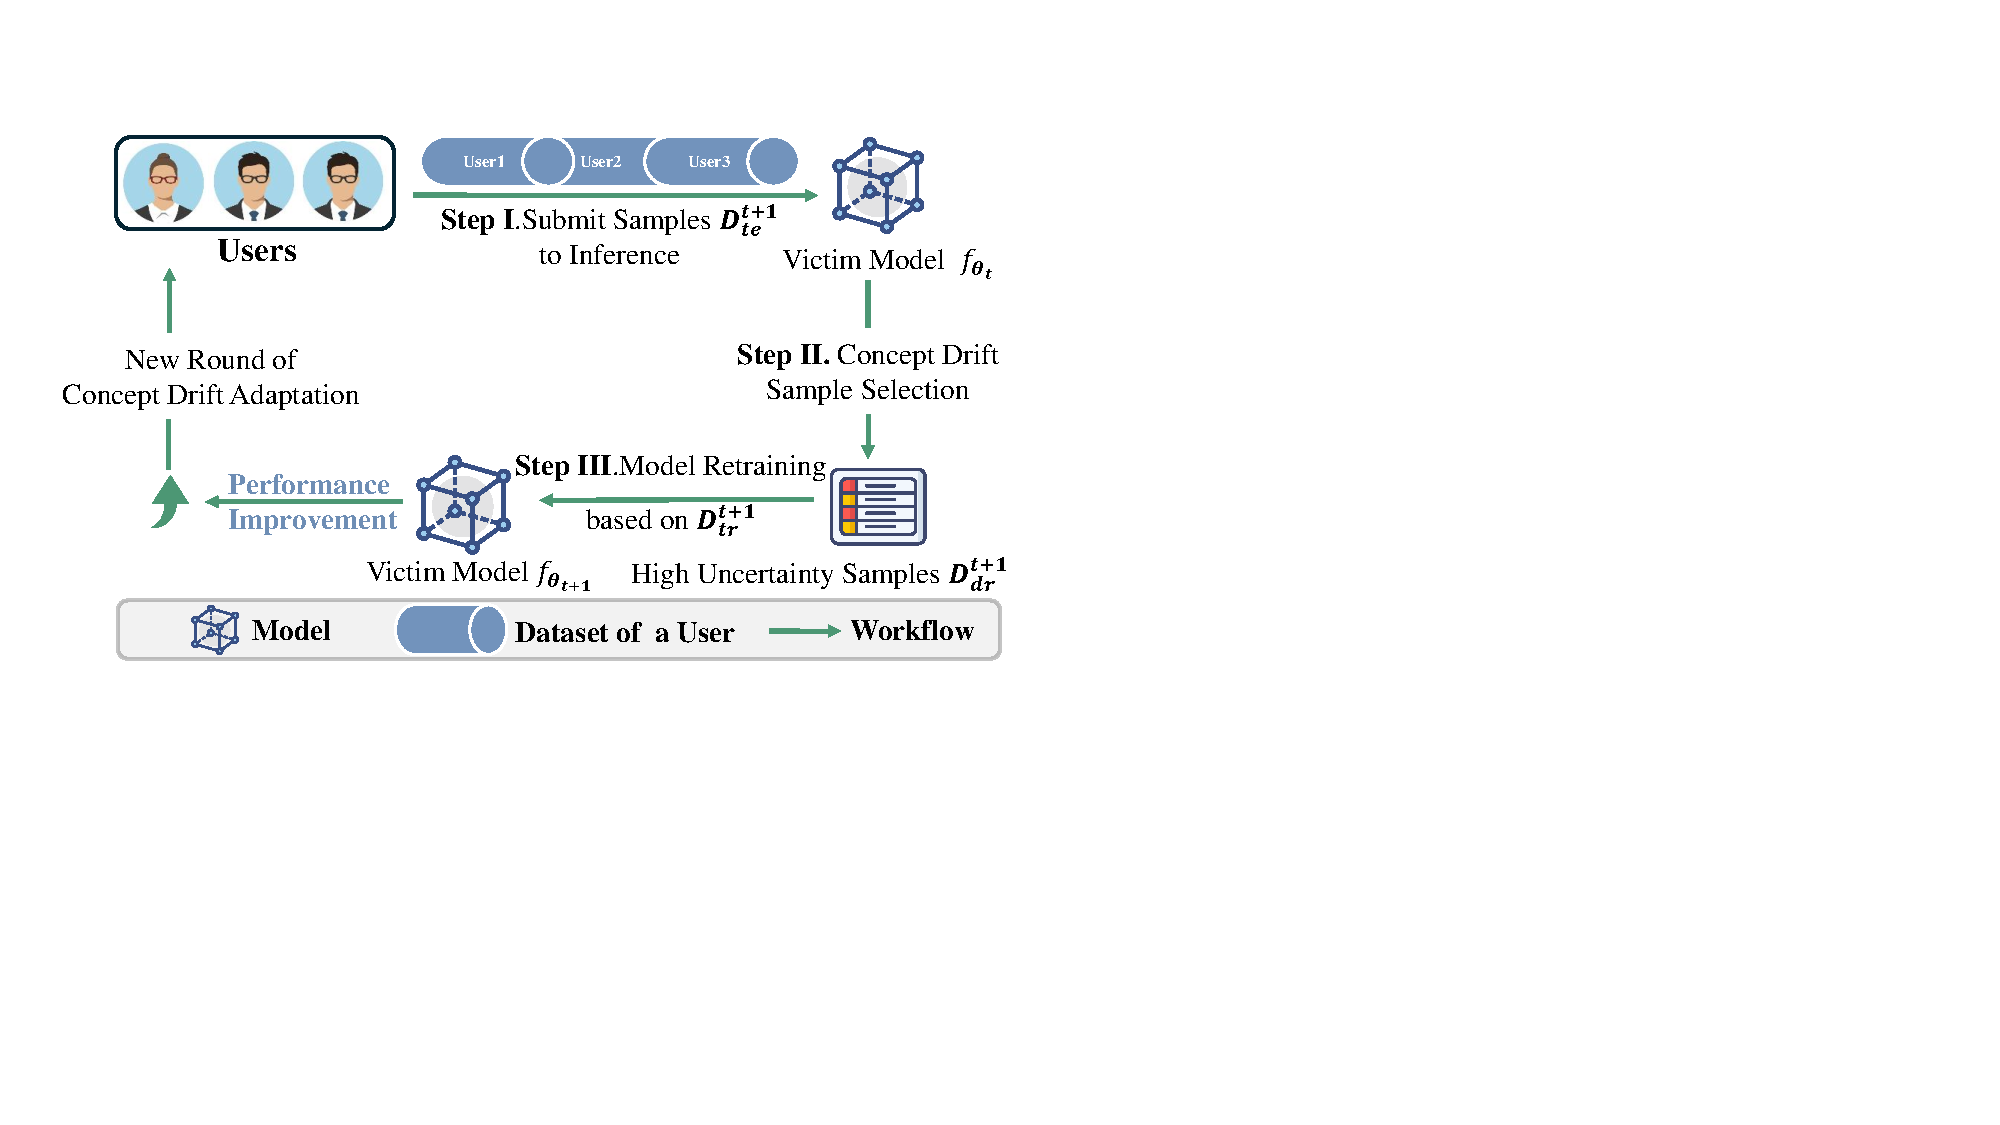
\includegraphics[width=\linewidth,keepaspectratio]{Graph/Intro_graph/Background/Concept_Drift_Adaptation_Based_Active_Learning_2025_3_27_15_23.pdf}
%	\caption{Concept drift adaptation based active learning}
%	\label{fig: CDA-AL-1}
%\end{figure}
%The overall process is illustrated in Figure~\ref{fig: CDA-AL-1}.
For consistency, we refer to the concept drift adaptation model as the victim model throughout this paper.
The entire concept drift process is composed of multiple concept drift cycles.
%The number of concept drift cycles is set to $n$ in our subsequent discussions.
Let $f_{\bm{\theta}_{n}}$ denote the victim model trained on the training data $\bm{D}^{n}_{tr}$ in concept drift cycle $n$.
$\bm{\theta}_{n}$ denotes the retrained model parameters at the end of concept drift cycle $n$, while $\bm{D}^{n}_{tr}$ refers to the updated training dataset used by the victim model during that cycle.
The unlabeled testing dataset $\bm{D}_{te}^{n}$ comprises all samples collected by the victim model throughout concept drift cycle $n$.
For concept drift cycle $n$, the concept drift adaptation process generally consists of three steps:

\emph{Step I}: Victim Model $f_{\bm{\theta}_{n-1}}$ performs inference on the input $\bm{\mathrm{x}}_{i} \in \bm{D}_{te}^{n}$ and obtain the classification confidence vector $\bm{\mathrm{c}}_{i} = f_{\bm{\theta}_{n-1}} \left( \bm{\mathrm{x}}_{i} \right)$.
	The different dimensions of $\bm{\mathrm{c}}_{i}$ indicate the model's confidence that the input $\bm{\mathrm{x}}_{i}$ belongs to a specific sample label. 
	The label with the highest confidence is selected as the predicted label $\overline{y}_{i}$ on the input $\bm{\mathrm{x}}_{i}$.

\emph{Step II}: %Based on the confidence vector $\bm{\mathrm{c}}_{i}$ obtained in the previous step, 
	The uncertainty score $\bm{\mathrm{u}}_{i}$ of $\bm{\mathrm{x}}_{i}$ is measured.
	For example, uncertainty can be measured as one minus the maximum softmax output of the network~\cite{2023-Usenix-chenyizhen}:
$\bm{\mathrm{u}}_{i} = 1-\max(\bm{\mathrm{c}}_{i},1-\bm{\mathrm{c}}_{i})$.
	%In addition to the commonly used confidence-based method described above, there are various other approaches for uncertainty quantification.
	%For details, see Section~\ref{Sec: Attack Influencing Factors}.
	We use $uncer()$ to denote uncertainty measures in the following discussion.

\emph{Step III}: High-uncertainty samples are selected from the testing data $\bm{D}_{te}^{n}$ as concept drift samples $\bm{D}_{dr}^{n}$.
	The size of $\bm{D}_{dr}^{n}$ is determined by the manual labeling capacity, referred to as the labeling budget $\beta$.
	Then, the concept drift data $\bm{D}_{dr}^{n}$ is manually labeled to get the ground truth label and added to the existing training data $\bm{D}^{n-1}_{tr}$ to form an updated training data $\bm{D}^{n}_{tr} = \bm{D}_{tr}^{n-1} \cup \bm{D}_{dr}^{n}$.
	The victim model $f_{\bm{\theta}_{n-1}}$ is then retrained on the updated training data $\bm{D}^{n}_{tr}$ to yield an updated model $f_{\bm{\theta}_{n}}$, as described in Equation~\ref{active learning loss}.
	\begin{equation}
		\begin{aligned}
			\bm{\theta}_{n} = \arg\min_{\bm{\theta}_{n-1}} \sum_{\bm{\mathrm{x}}_{i} \in \bm{D}^{n}_{tr}} \mathcal{L} \left( f_{\bm{\theta}_{n-1}}\left( \bm{\mathrm{x}}_{i}\right) , y_{i}  \right) \\
		\end{aligned}
		\label{active learning loss}
	\end{equation}


%\textbf{didn't you already mention this??? what is the point of this paragraph??}
%In this paper, we refer to the samples selected by the uncertainty-based selection strategy as concept drift samples, although they may not be directly affected by drift.
%Uncertainty can also result from other factors, such as when samples lie near the decision boundary in a stable distribution.
%Following prior work~\cite{2023-Usenix-chenyizhen}, we do not explicitly distinguish these samples in the following discussion since such differentiation pertains to concept drift detection rather than adaptation.


\subsection{Data Poisoning Attacks}
\label{Sec: Data Poisoning Attacks}

In data poisoning attacks, the attacker constructs poisoned data to degrade the performance of the victim model.
The most common strategy is to inject poisoned samples into the victim model  training data.
As noted by Tian et al.~\cite{2022-ACM-Computing-Survey-Poisoning-attacks-and-countermeasures-in-ML} and Wang et al.~\cite{2022-ACM-Computing-Survey-Threats-to-training}, such attacks are generally categorized as targeted or untargeted.
Untargeted poisoning attacks aim to hinder the convergence of the victim model and eventually lead to denial-of-service~\cite{pmlr-v20-biggio11,2023-AAAI-yuuntargeted,wang2023analysis}.
The challenge with untargeted attacks is that they aim to degrade the performance across all data~\cite{2024-CCS-Phantom}.
Therefore, the effect of poisoned samples must outweigh that of the clean training data.
In contrast, targeted poisoning attacks aim to manipulate the victim model into making incorrect predictions on specific inputs~\cite{2024-TIFS-Backdoor-Contrastive-Learning,2021-Usenix-Poisoning-Attack-Explanation-guided-Backdoor,2023-SP-backdoor-attack}.
The inputs for which the model  predictions are compromised are called attack targets. 
To launch a targeted poisoning attack, an adversary needs to
inject malicious knowledge into the training data while keeping other knowledge unaffected~\cite{2022-ACM-Computing-Survey-Poisoning-attacks-and-countermeasures-in-ML}.

		
		%DIF < \input{ThreatModel0}
\DIFdelbegin %DIFDELCMD < 

%DIFDELCMD < %%%
\DIFdelend \section{Threat Model\DIFdelbegin \DIFdel{, Design Challenegs and Overview of PACDA}\DIFdelend }
\DIFdelbegin %DIFDELCMD < \label{Sec: Attack Method}
%DIFDELCMD < 

%DIFDELCMD < %%%
\DIFdel{In this section, we present the threat model, the design rationale behind the attack, and an overview of PACDA.
}%DIFDELCMD < 

%DIFDELCMD < %%%
\subsection{\DIFdel{Threat Model}}
%DIFAUXCMD
\addtocounter{subsection}{-1}%DIFAUXCMD
\DIFdelend \label{Sec: Threat Model}

% 2024-12-11-14-20-閲嶆柊鏁寸悊濞佽儊妯″瀷
%\subsection{Attacker Goal}
Similar to previous research~\cite{2023-TIFS-person-re-identification-backdoor,2018-NIPS-Poison-frogs}, attackers'goal is to ensure that the victim model consistently misclassifies the attack target throughout the CDA-AL process.
The attacker will also attempt to keep the victim model  overall performance stable, thereby maintaining the stealth of the attack.
In addition, it is important to note that in the PACDA, the attack target has a defined source class but does not enforce misclassification into a specific target class.
By avoiding a fixed target class, this class-agnostic misclassification strategy increases the difficulty of detection, as the victim model is more likely to interpret the misclassifications as effects of natural concept drift or inherent uncertainty rather than deliberate poisoning attack.

%\subsection{Attacker Capabilities}
We assume attackers cannot access the victim model's internal parameters or influence its training process, including manual labeling~\cite{9663183}.
Attackers can only submit samples to the victim model for querying to obtain outputs such as sample uncertainty scores and predicted labels.
Additionally, attackers are presumed to have access to public data and the resources required to train surrogate models~\cite{Qin_Xiong_Yi_Hsieh_2023,10.1145/3052973.3053009}.
Consistent with previous research on active learning attacks~\cite{2021-Usenix-active-learning-backdoor}, we assume the attacker typically has knowledge of the victim model's labeling budget settings. %(including the uncertainty threshold).
\DIFaddbegin \DIFadd{Moreover, the attacker can access the victim model  prediction uncertainty.
This is based on the observation that many existing machine learning services (e.g., image recognition platforms~\mbox{%DIFAUXCMD
\cite{2025-Baidu-Image-Recognition}}\hskip0pt%DIFAUXCMD
) provide uncertainty information to help users better interpret and utilize the prediction results.
Similarly, malware detection services such as VirusTotal~\mbox{%DIFAUXCMD
\cite{Virustotaluploadinterface} }\hskip0pt%DIFAUXCMD
provide outputs from multiple detection models, enabling users to estimate prediction uncertainty based on the distribution of these results.
}

\DIFaddend %Furthermore, in Section~\ref{Sec: Attack Influencing Factors}, we perform an experimental analysis for the scenario where the attacker cannot access the victim model's labeling budget to understand how this capability affects the attack success rate.
\DIFaddbegin \DIFadd{Moreover, it is important to note that although CDA-AL systems involve human analysts, their primary role is to provide reliable labels for concept drift samples. As long as PACDA does not rely on assumptions such as label flipping, the attack remains inconspicuous to human analysts.
		}\DIFaddend 

		\DIFaddbegin \section{\DIFadd{Design Challenges and Overview of PACDA}}
\label{Sec: Attack Method}

\DIFadd{In this section, we present the threat model, the design rationale behind the attack, and an overview of PACDA.
}

\DIFaddend \subsection{Design Challenges}

PACDA faces three key challenges.
(1) The sample selection strategy deployed in CDA-AL restricts the arbitrary injection of poisoned samples into the training data.
Therefore, attackers must ensure that the victim model selects poisoned samples for labeling.
(2) The sample labeling process in active learning is based on manual analysis, meaning the labels of all poisoned samples in the training data must remain correct.
The attacker cannot degrade the victim model  concept drift adaptation performance by tampering with the sample labels~\cite{2018-NIPS-Poison-frogs,2019-NIPS-Transferable-clean-label-poisoning-attacks-on-deep-neural-nets}.
(3) Existing targeted poisoning attacks are typically evaluated for effectiveness on models with fixed parameters. 
For example, backdoor attacks are often evaluated on pre-trained models~\cite{2024-TIFS-Backdoor-Contrastive-Learning,2021-Usenix-Poisoning-Attack-Explanation-guided-Backdoor,2023-SP-backdoor-attack}.
In contrast, PACDA must ensure its attack remains effective as the victim model continuously updates its parameters.
PACDA tackles the first two challenges.
The final challenge is addressed through continuous attacks on the concept drift adaptation process.
%Additionally, we validate the persistence of the attack  effectiveness on concept drift data spanning seven years, as discussed in Section~\ref{Sec: Single Attack Targets}.

\subsection{Design Rationale}
The key issue is ensuring that the poisoned samples have high uncertainty.
Prior research has demonstrated that uncertainty quantification techniques are vulnerable to manipulation by adversaries~\cite{Ledda_2023_ICCV}.
Specifically, Ledda et al. employed perturbation search techniques to find the minimal perturbations capable of altering a sample's uncertainty~\cite{Ledda_2023_ICCV}.
However, their method focuses on reducing uncertainty, whereas CDA-AL selects samples with high uncertainty~\cite{2023-Usenix-chenyizhen}.
Inspired by Yang et al. and Chen et al., who represent sample uncertainty by measuring the similarity between testing and training data~\cite{2021-Usenix-CDAE,2023-Usenix-chenyizhen}, we find that newly appearing concept drift samples always inherently exhibit high uncertainty.
This is primarily because of their low similarity to the existing training data.
Therefore, our attack exploits the inherent high uncertainty of concept drift samples to craft poisoned samples that are likely to be selected for labeling, thereby exhausting the labeling budget and preventing the victim model from learning the attack target.

\subsection{Overview of PACDA}
Based on the design rationale, we propose the PACDA framework, illustrated in Figure~\ref{fig:Attack Process}.
First, we perform a value assessment of the attack target to avoid wasting limited attack resources on targets that do not hold attack value.
Next, we estimate the required budget consumption for labeling based on the selected attack target.
By controlling the budget consumed, the attacker determines which knowledge the victim model can or cannot acquire.
Subsequently, we define the search constraints and identify high-uncertainty samples from the testing data as poisoning seeds to consume the victim model  labeling budget.
We then perform uncertainty-based feature attribution on selected testing samples to prepare for the subsequent generation of poisoned samples.
As the number of such seeds is often insufficient to fully consume the labeling budget, we further adopt a poisoned sample generation strategy.
PACDA provides two generation strategies.
Strategy II enhances Strategy I but incurs higher cost.
The attacker selects between them based on knowledge of the attack target (e.g., uncertainty ranking).
Ultimately, PACDA exhausts the victim model  labeling budget, preventing effective learning of the attack target.
\begin{figure}[t]
	\centering
	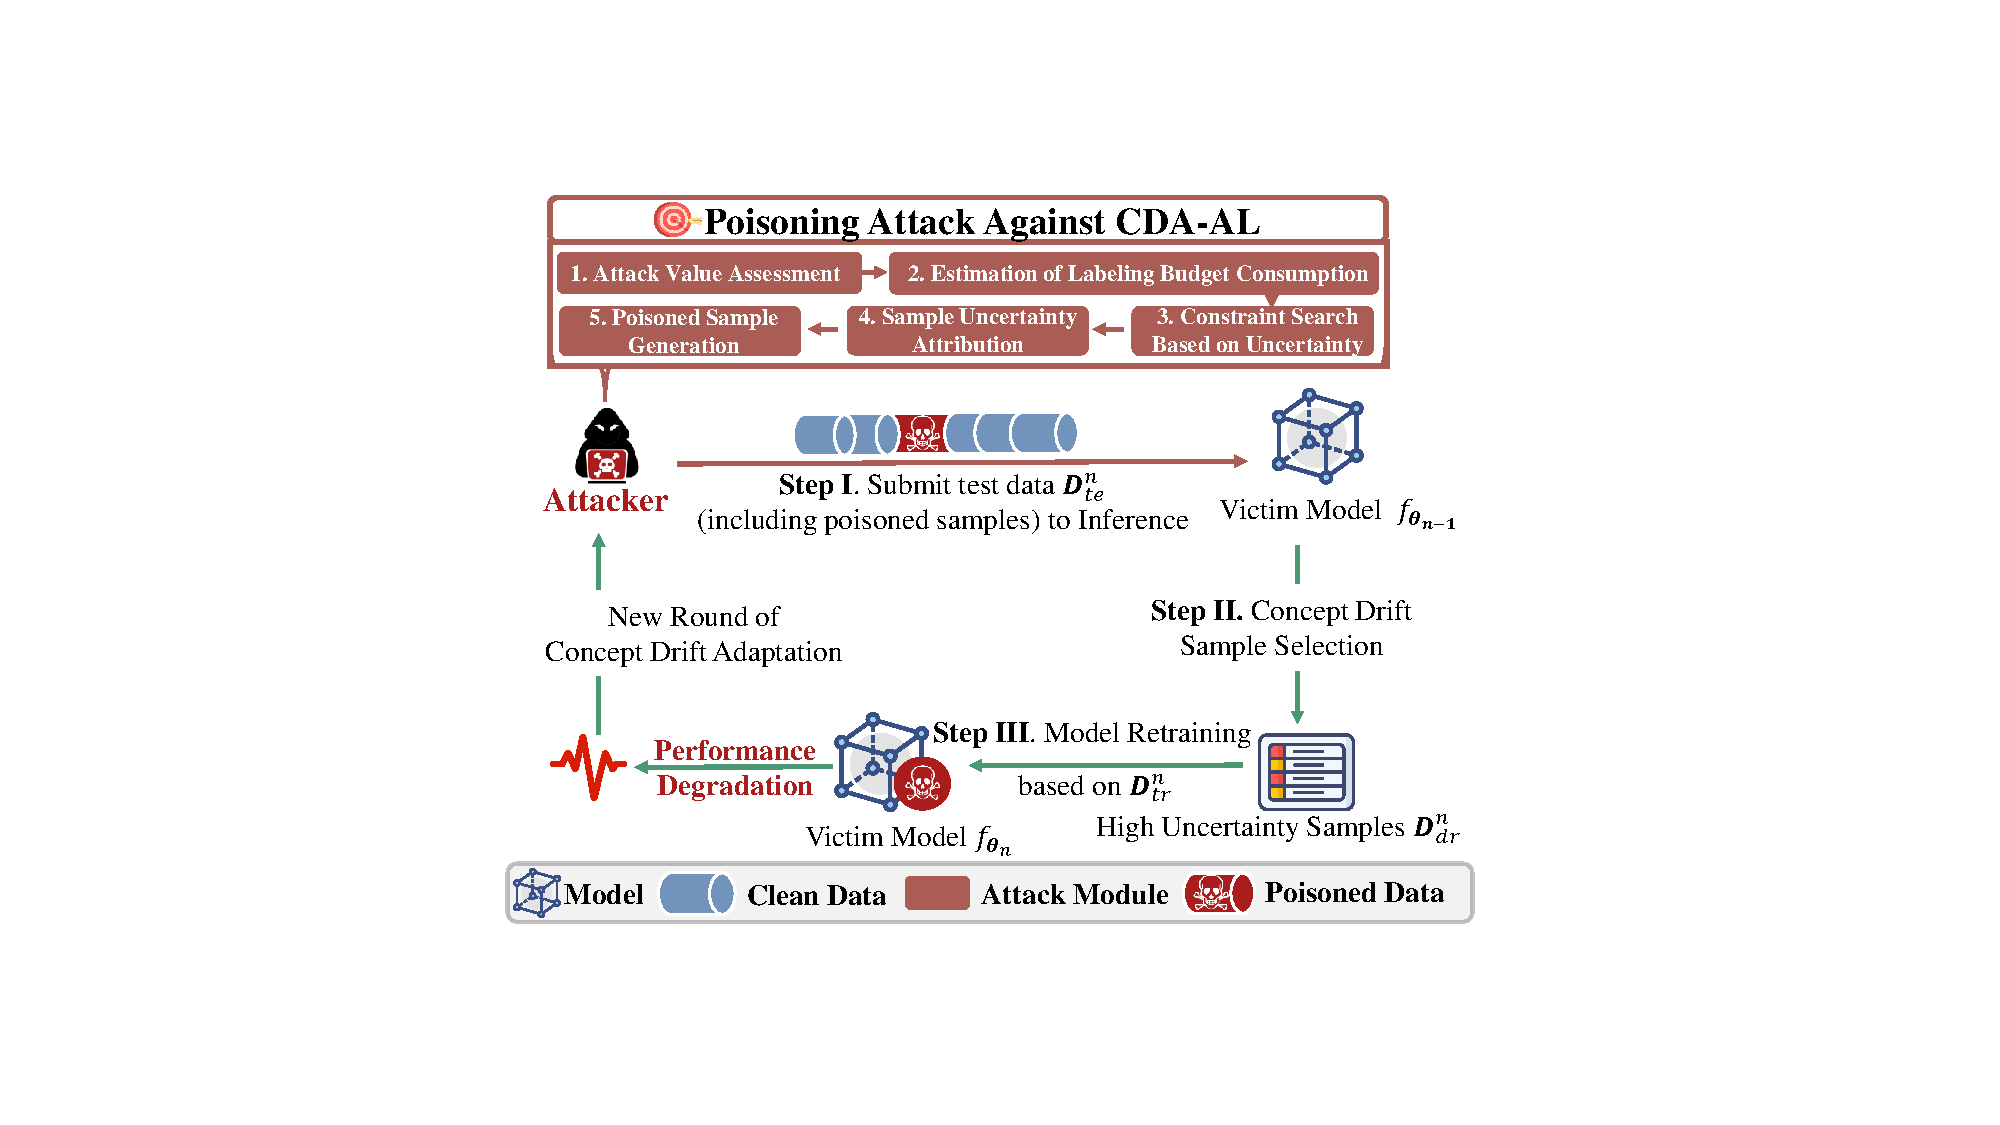
\includegraphics[width=\linewidth,keepaspectratio]{Graph/Attack_Method/PACDA_attack_process_2025_4_23_01_06.pdf}
	\caption{Poisoning Attack against CDA-AL}
	\label{fig:Attack Process}
\end{figure}

\section{Detailed Design of PACDA}
\label{Sec: Detailed Design of PACDA}

We demonstrate the design of the PACDA method by using concept drift cycle $n$ as an example, executing the same attack procedure in every concept drift cycle.
In concept drift cycle $n$, the complete testing dataset collected by the victim model is denoted as $\bm{D}_{te}^{n} \in \mathbb{R}^{N \times d}$ (with N samples in d dimensions).
The attack target sample $\bm{\mathrm{x}}_{tar}$ is a member of the testing data $\bm{D}_{te}^{n}$. 
The victim model is denoted as $f_{\bm{\theta}_{n-1}}$, and its labeling budget is represented by $\beta$.
Notably, at the start of concept drift cycle $n$, the victim model is derived from the model updated at the end of concept drift cycle $n-1$. Therefore, the model parameters at this stage are denoted as $\bm{\theta}_{n-1}$.
The victim model performs uncertainty quantification on the collected testing data and ranks the samples accordingly.
The top $\beta$ samples with the highest uncertainty ranking are selected for manual analysis to obtain the concept drift data $\bm{D}_{dr}^{n} \in \mathbb{R}^{\beta \times d}$ (with $\beta$ samples in d dimensions).

\subsection{Attack Value Assessment}
\label{Sec: Attack Value Assessment}
The PACDA is essentially a resource-exhaustion attack that targets the labeling budget of the victim model.
However, the attacker also faces similar risks of resource exhaustion.
For example, resources may be wasted if the attacker chooses a attack target already in the training data.
A failed attack prevents the attacker from obtaining any reward and incurs substantial attack costs.
Consequently, the attacker must carefully assess whether the attack target is worth attacking.
This decision is based on the accuracy of the victim model  prediction of the attack target.
Samples not present in the training data are more likely to be misclassified, making this a strong indicator of attack value.
The attacker can leverage the victim model to make this determination.
If the predicted label $\overline{y}_{i}$ of $\bm{\mathrm{x}}_{tar}$ from the victim model $f_{\bm{\theta}_{n-1}}$ differs from the ground-truth label $y_{i}$, the attack target is likely to be of high attack value.

\subsection{Estimation of Labeling Budget Consumption}
\label{Sec: Surrogate Model Training}
Once the attack target is determined to be valuable, the PACDA begins by estimating the amount of the labeling budget that needs to be exhausted from the victim model.
The attacker makes decisions based on the uncertainty ranking of the attack target.
If the uncertainty ranking $r_{tar}$ of the attack target is higher than the labeling budget boundary $(r_{tar} < r_{\beta})$, the attack target will be selected as a concept drift sample.
It is important to note that a higher uncertainty ranking corresponds to a smaller value of $r_{tar}$.
Then, the attack target will be learned during the retraining process of the victim model.
The gap between the uncertainty ranking of the attack target and the labeling budget boundary represents the primary objective of the attacker  labeling budget consumption, denoted as $C_{n}$.
It also reflects the minimum requirement for the number of poisoned samples.
When $r_{tar} > r_{\beta}$, it indicates that the attack target $\bm{\mathrm{x}}_{tar}$ will not be selected by the victim model $f_{\bm{\theta}_{n-1}}$.
Nonetheless, the attacker will still generate some poisoned samples, even if the attack target is not selected.
This mitigates potential mismatches between the attacker  and the victim  testing data, which could otherwise cause the attacker to overestimate the target  uncertainty ranking.
Therefore, to ensure reliability, the consumption of the labeling budget is set to a fixed value $\lambda \, (\lambda \ll \bm{D}_{te}^{n})$, determined by the attacker  computational resources.
Specifically, the amount of budget consumption $C_{n}$ for labeling is as follows:
\begin{align}
	C_{n} =
	\begin{cases} 
		(r_{\beta}-r_{tar}) + 1, \; r_{tar} < r_{\beta} \\
		\lambda , \; r_{tar} > r_{\beta}
	\end{cases}
\end{align}

\subsection{Constraint Search based on Uncertainty Ranking}
The attacker then searches the testing data $\bm{D}_{te}^{n}$ for naturally occurring samples that can be used to exhaust the victim model  labeling budget $C_{n}$.
These selected samples are referred to as poisoning seed samples.
The poisoning seed data, denoted as $\bm{D}_{seed}^{n} \in \mathbb{R}^{K \times d}$ (with $K$ samples in d dimensions), consists of samples that satisfy the uncertainty criterion defined in Equation~\ref{equncer}.
We denote each row of the testing data as a sample vector $\bm{\mathrm{x}}_{i}$, where $\bm{\mathrm{x}}_{i} = \bm{D}_{te,\,i*}^{n}$,$\forall i \in \{0, \dots, N-1\}$.
The uncertainty of these poisoned seed samples must exceed the attack target  uncertainty, as shown below.
\begin{equation}
	\begin{aligned}
		uncer(f_{\bm{\theta}_{n-1}} \left( \bm{\mathrm{x}}_{i} \right)) > uncer(f_{\bm{\theta}_{n-1}} \left( \bm{\mathrm{x}}_{tar} \right))
	\end{aligned}
	\label{equncer}
\end{equation}
Furthermore, it is crucial to ensure that the poisoned samples exhaust the victim model  labeling budget without enhancing its concept drift adaptation capability.
For instance, incorporating novel malware samples into the poisoning seed data may improve the victim model  ability to detect malicious behavior, thereby undermining the attacker  objective of causing misclassification of the attack target.
Therefore, the attacker must remove malware samples from the attack seed data to avoid reducing the attack success rate on the attack target.
In addition, similarity-based filtering can be employed to prevent the inclusion of samples similar to the attack target in the poisoned samples.
\begin{equation}
	\begin{aligned}
		(y_{j} \neq y_{tar}) \land [sim(\bm{\mathrm{x}}_{j},\bm{\mathrm{x}}_{tar})< \tau]
	\end{aligned}
	\label{E6}
\end{equation}
Each row of the poisoning seed data $\bm{D}_{seed}^{n}$ is denoted as a sample vector $\bm{\mathrm{x}}_{j}$, where $\bm{\mathrm{x}}_{j} = \bm{D}_{\text{seed}}^{n}[j,:]$,$\forall j \in \{0, \dots, K-1\}$.
The constraint condition applied to each sample vector $\bm{\mathrm{x}}_{j}$ is defined in Equation~\ref{E6}.
Samples that do not satisfy this condition are removed from the poisoning seed data $\bm{D}_{seed}^{n}$.
Finally, the refined poisoning seed data is sorted in descending order of uncertainty, with the sample at index 0 having the highest uncertainty.

\subsection{Sample Uncertainty Attribution}
\DIFdelbegin \DIFdel{Next, the attacker constructs an uncertainty interpreter based on }\DIFdelend \DIFaddbegin \DIFadd{After obtaining the poisoned seed samples $\bm{D}_{seed}^{n}$, we aim to interpret their high uncertainty to facilitate the subsequent poisoned sample generation by expanding the space of manipulable uncertainty rankings.
Given the need to accommodate various concept drift models, our uncertainty attribution method should be model-agnostic.
Moreover, to effectively construct poisoned samples with high uncertainty, the explanation should operate at the feature level.
Although standard conformal prediction methods can provide interpretable uncertainty estimates through credibility scores, they are unable to offer feature-level explanations of uncertainty.
Therefore, we adopt a }\DIFaddend Shapley Additive Explanations (SHAP) \DIFdelbegin \DIFdel{to facilitate the subsequent poisoned sample generation strategy}\DIFdelend \DIFaddbegin \DIFadd{based approach for feature level attribution of sample uncertainty}\DIFaddend .
The fundamental concepts of SHAP are provided in Appendix~\ref{Sec: Shapley Additive Explanations}.
We utilize a standardized permutation-based SHAP method to interpret sample uncertainty, approximating shapley values by iterating through permutations of input features.
This model-agnostic explainer ensures local accuracy (additivity) by iterating completely through an entire permutation of the features in both forward and reverse directions (antithetic sampling).
Since the objective of the attack is to prevent the victim model from learning the attack target, the generated poisoned samples must suppress the model  ability to adapt to concept drift.
To achieve this, samples outside the labeling budget are selected as targets for feature space perturbation.
Their lower importance relative to in-budget samples helps avoid inadvertently strengthening the model  adaptation capabilities.
The attacker applies uncertainty feature attribution on the testing data outside the labeling budget, denoted as $\bm{D}_{shap}^{n}$ ($\bm{D}_{shap}^{n} = \bm{D}_{te}^{n} \setminus \bm{D}_{dr}^{n}$).
These samples are then sorted in descending order based on their uncertainty scores.
\begin{equation}
	\begin{aligned}
		 \bm{V}_{shap} = SHAP (\bm{D}_{tr}^{n-1},UncerSort(\bm{D}_{shap}^{n})) \\
	\end{aligned}
\end{equation}
$\bm{V}_{shap}$ represents the matrix of uncertainty feature attributions for data $\bm{D}_{shap}^{n}$.
$\bm{\mathrm{v}}_{i}$ denotes the feature attribution vector of a specific sample, while $v_{i,j}$ indicates the impact of a particular feature on the uncertainty of the given sample.

\subsection{Poisoned Sample Generation}
\label{Sec: Poisoned Sample Generation}
The poisoned seed samples $\bm{D}_{seed}^{n}$ is incorporated into the victim model  training data due to its high uncertainty.
However, the seed samples obtained via the constrained search strategy may not fully satisfy the required labeling budget consumption $C_{n}$ of the victim model.
Consequently, attack targets $\bm{\mathrm{x}}_{tar}$ will still be selected and labeled manually, leading to a failure of the PACDA.
To ensure the effectiveness of the PACDA, the attacker must generate an additional batch of poisoned samples such that the total number of poisoned samples is greater than or equal to the labeling budget consumption $C_{n}$.

\subsubsection{Selection of Poisoned Sample Generation Strategy}
\label{Sec: Selection of Poisoned Sample Generation Strategy}

We propose two poisoned sample generation strategies: Strategy I, which is based on problem-space perturbation, and Strategy II, which leverages Shapley additive explanations.
Both strategies aim to generate poisoned samples that consume the labeling budget, thereby leading to misclassification of the attack target.
However, the two strategies are suitable for different types of attack targets.
Strategy I prevents the victim model from learning specific knowledge about the attack target by constructing poisoned samples without introducing incorrect concept drift information.
It focuses solely on preventing the victim model from learning the attack target while minimizing its impact on the model  ability to adapt to concept drift.
In contrast, Strategy II prevents the victim model from acquiring knowledge about the attack target and introduces misleading information about concept drift into the training process.
Although this reduces the model  ability to adapt to true concept drift in the testing data, it does not cause a significant drop in overall performance, as indicated by the F1 score in Table~\ref{tab:Attack Effectiveness}.

In terms of strategy selection, Strategy I is better suited for attack targets that are inherently challenging to learn, typically those exhibiting a high degree of concept drift.
Conversely, when the attack target is relatively easy to learn due to weak concept drift, strategy II is employed to enhance the effectiveness of the attack.
Finally, we ensure that, regardless of the degree of concept drift exhibited by the attack target, the victim model fails to learn the attack target due to its inability to efficiently allocate the limited labeling budget, ultimately leading to the misclassification of the attack target.

\subsubsection{Problem-Space Perturbation (Strategy I)}
\label{Sec: Strategy I-Problem-Space Perturbation}

Specifically, Strategy I is particularly effective for rapidly and cost-efficiently adjusting the uncertainty rankings of samples within the labeling budget.
%For instance, consider a sample $\bm{\mathrm{x}}_{A}$ from the poisoning seed data $\bm{D}_{seed}^{t+1}$.
%Let the attack target be denoted by $\bm{\mathrm{x}}_{tar}$.
%Their respective uncertainty rankings are $r_{A}$ and $r_{tar}$, respectively, and their uncertainty scores are $u_{A}$ and $u_{tar}$ ,with $u_{A} > u_{tar}$.
%By applying problem space perturbation to sample $\bm{\mathrm{x}}_{A}$, we can generate a poisoned sample that maintains a similar uncertainty level $u_{A}$.
The problem space perturbation strategy refers to modifying the samples in the poisoning attack seed data $\bm{D}_{seed}^{n}$ to generate new poisoned samples without altering the features of the samples.
We denote each row of the attack seed data $\bm{D}_{seed}^{n}$ as a sample vector $\bm{\mathrm{x}}_{k}$, where $\bm{\mathrm{x}}_{k} = \bm{D}_{\text{seed}}^{n}[k,:]$,$\forall k \in \{0, \dots, M-1 \}$.
Due to the need for attack stealth, the samples generated by problem space perturbation must minimize the impact on other concept drift samples. 
Therefore, we select the $\epsilon$ least uncertain samples from the poisoned seed sample set for problem space perturbation. 
The smaller $\epsilon$ is, the lesser the impact on existing concept drift samples.
In this paper's subsequent attack effectiveness evaluation, we set $\epsilon$ to 5, which accounts for 0.025 of the labeling budget.
A perturbation in the problem space is applied to these samples $\bm{\mathrm{x}}_{k}$, $k \in \{0, \dots,  \epsilon-1 \}$ , resulting in a new data denoted as $\bm{D}_{\alpha}^{n}$.
$\alpha$ denotes the problem-space perturbation operations, as shown in Table~\ref{tab: List of Problem Space Perturbation Operations}.
This strategy ensures that the newly generated poisoned samples exhibit high uncertainty, thereby maintaining their potential to exhaust the victim model  labeling budget and increase the uncertainty ranking of the attack target $r_{tar}$ beyond the labeling budget (i.e., $r_{tar} > r_{\beta}$).
\begin{table}[h!]
	\caption{Problem-Space Perturbation Operations}
	\label{tab: List of Problem Space Perturbation Operations}
	\setlength{\tabcolsep}{5.8pt}
	\begin{center}
		\scalebox{1.0}{
			\begin{tabular}{cc}
				\toprule
				\textbf{Dataset} & \textbf{Perturbation Operations ($\alpha$)}\\
				\midrule
				APIGraph & Rename method names to meaningless identifiers  \\ 
				\specialrule{0.05em}{1pt}{1pt}
				APIGraph & Modify image and other resource files     \\ 
				\specialrule{0.05em}{1pt}{1pt}
				BODMAS & Modify the system API function names   \\
				\specialrule{0.05em}{1pt}{1pt}
				BODMAS & Dynamically adjust the size of the DOS STUB space  \\
				\specialrule{0.05em}{1pt}{1pt}
				MNIST & Add Gaussian noise to the image pixels  \\
				\specialrule{0.05em}{1pt}{1pt}
				MNIST & Apply sharpening to enhance the edges of the image  \\
				\specialrule{0.05em}{1pt}{1pt}
				SPAM & Remove non-essential words \\
				\specialrule{0.05em}{1pt}{1pt}
				SPAM & Insert random symbols or additional spaces  \\
				\bottomrule
		\end{tabular}}
	\end{center}
\end{table}

The reason is that machine learning models, during the feature extraction process, often ensure that non-critical perturbations $\alpha$ in the data do not affect the features in order to construct robust representations.
Therefore, when the attacker adjusts the non-essential information of a sample, the sample is altered, but its features remain unchanged.
Since existing uncertainty quantification methods are based on sample features, altering the problem space does not reduce the sample's uncertainty, ensuring that the labeling budget can be exhausted.
For example, in software applications, when key information such as permissions and API calls is extracted as features, elements like icon usage, coding style, and redundant code have no direct relationship with these critical features.
Examples of problem space perturbations in different domains can be found in Table~\ref{tab: List of Problem Space Perturbation Operations}.
All perturbation operations preserve the original labels of the poisoned seed samples.
The perturbation operation in the problem space is infinite, allowing for generating a sufficient number of poisoned samples.
Thus, by leveraging high-uncertainty seed samples $\bm{D}_{seed}^{n}$ and the problem space perturbation strategy, the attacker can generate poisoned samples $\bm{D}_{\alpha}^{n}$ to meet the victim model's labeling budget consumption requirements $C_{n}$.
This attack strategy generates poisoned samples quickly and is low-cost, making it the preferred choice for most attack targets.
As long as the poisoned sample seed set is not empty, problem space perturbation can be applied.

\subsubsection{Feature-Space Perturbation (Strategy II)}
\label{Sec: Strategy II: Feature-Space Perturbation}

However, the uncertainty of poisoned samples generated through problem space perturbation is limited by the uncertainty of the seed samples from $\bm{D}_{seed}^{n}$.
Thus, it is difficult to affect samples with higher uncertainty than the poisoned seed samples.
If the portion of the labeling budget with higher uncertainty than the poisoning seed samples contains samples that hinder the misclassification of the attack target (e.g., malware using similar vulnerabilities as the target), the attack success rate may decrease.
We introduce a feature space perturbation method (Strategy II) based on the uncertainty attribution matrix $\bm{V}_{shap}$ to overcome this limitation.
This approach removes the upper bound constraint on poisoned sample uncertainty imposed by the poisoned seed samples.
It is worth noting that the uncertainty attribution matrix allows samples originally outside the labeling budget to be shifted into the budget through feature-space perturbation.
Consequently, the approach eliminates the dependence on high-uncertainty seed samples.
It enhances the attack  robustness by preventing the victim model from acquiring accurate knowledge of actual concept drift samples.
Feature space perturbation can not only overcome the inherent limitations of problem space perturbation but also be combined with it, making it a viable approach to further enhance the effectiveness of problem space perturbation strategies.
%So, the attacker can operate in two different attack modes based on the cost the attack service purchaser is willing to pay.
%The attacker can choose to use the problem space perturbation strategy alone. 
%This approach is low-cost, but the attack success rate on some attack targets cannot be guaranteed.
%If the attacker has sufficient computational resources and aims for a higher attack success rate, they can generate poisoned samples by applying feature space perturbations.

The uncertainty attribution module has obtained the uncertainty attribution matrix $\bm{V}_{shap}$.
We denote each row of the uncertainty attribution matrix as a vector $\bm{\mathrm{v}}_{i}$, where $\bm{\mathrm{v}}_{i} =\bm{V}_{\text{shap}}[i,:]$,$\forall i \in \{0, \dots, N-1 \}$.
Based on the uncertainty feature attribution vector $\bm{\mathrm{v}}_{i}$ for each sample, the attacker identifies the set of feature indices $\bm{I}_{shap}$ that have the greatest impact on increasing uncertainty.
The computation of the feature index vector $\bm{I}_{shap}$ is shown in Equation~\ref{mask}.
\begin{equation}
	\begin{aligned}
		\bm{I}_{shap} = \{ argsort(\bm{\mathrm{v}_{i}})[0:d-1]  \} \\
		\end{aligned}
	\label{mask}
\end{equation}
$d$ denotes the dimension of the feature vector for each sample.
The sorting function ranks feature indices based on their influence on sample uncertainty, such that features contributing more to increased uncertainty are assigned smaller index values.  
Therefore, the attacker can focus on modifying features with lower index values to effectively amplify uncertainty.
%As shown in Figure 4, the Force plot of the uncertainty feature attribution vector $\bm{\mathrm{v}}_{i}$ is ordered by the $\bm{I}_{shap}$ index.
%Red indicates features that increase the sample's uncertainty, while blue represents features that decrease it.
%The features closer to the center significantly impact uncertainty, corresponding to the lower-indexed parts of $\bm{I}_{shap}$.
%Modifying the features corresponding to the indices of the blue region will increase the sample uncertainty, as shown in Figure~\ref{fig:SHAP}.
We selected the top 2\% of features based on their indices for modification.
Since the uncertainty-based SHAP attribution provides a linear approximation of the model's predictive uncertainty, modifying the key features with the highest attribution values increases the sample's overall uncertainty.
%\begin{figure}[h!]
%	\centering
%	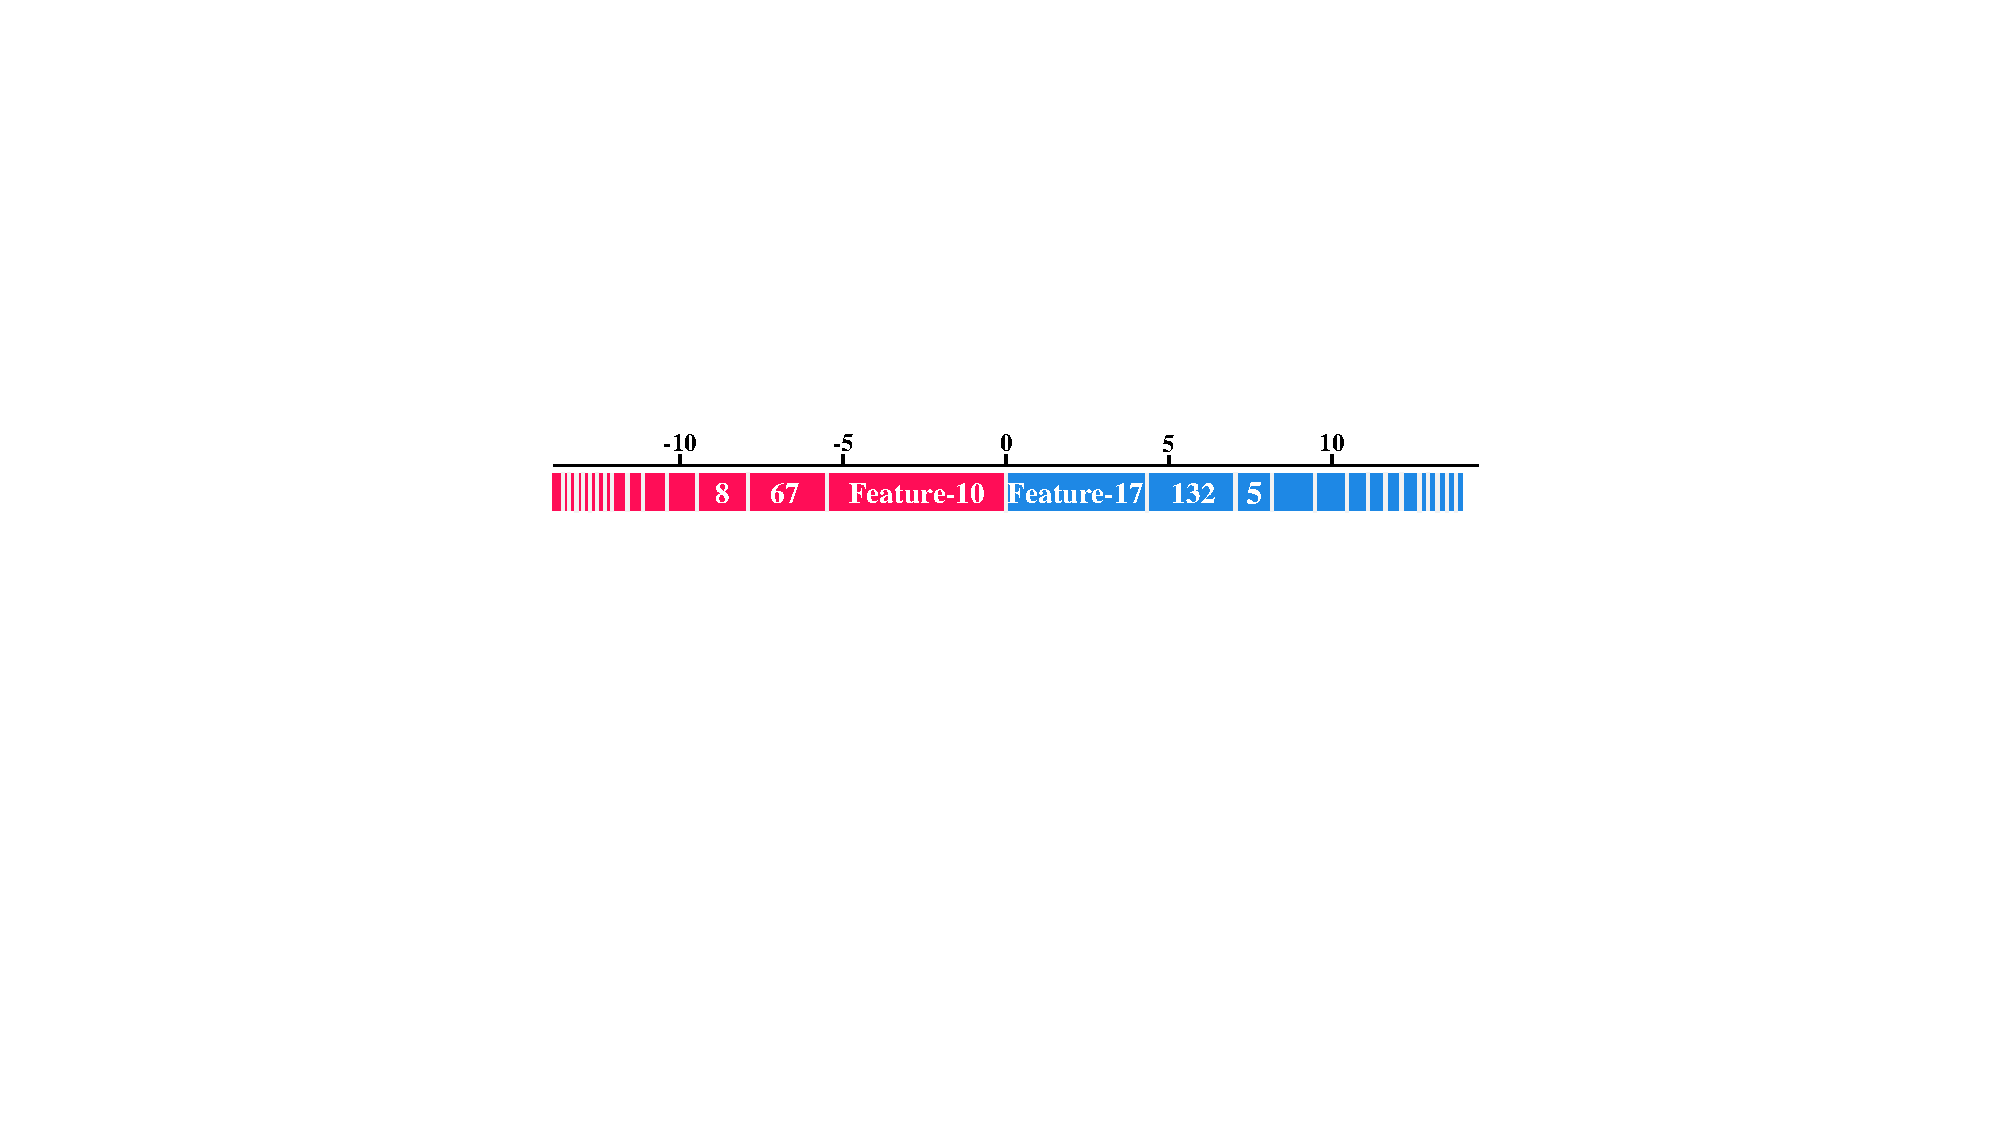
\includegraphics[width=\linewidth,keepaspectratio]{Graph/Evaluation/shap.pdf}
%	\caption{SHAP-based Sample Uncertainty Attribution}
%	\label{fig:SHAP}
%\end{figure}

A sample from the APIGraph dataset is taken as an example, and its features are represented as 0-1 vectors.
This feature modification corresponds to adjusting the API call patterns in the actual application.
Since the poisoned samples are intended to consume the labeling budget, the impact of the API calls on the program's functionality does not need to be considered.
Moreover, the modifications only reduce software API calls without introducing additional sensitive behaviors, thereby preserving the original label of the sample.
For data in other domains, we replace the values of the important features with the corresponding values from samples with high uncertainty.
The perturbed samples generated in this manner are considered as a new set of poisoned attack samples $\bm{D}_{shap}^{n}$.
Suppose the generated poisoned samples are smaller than the labeling budget consumption requirements $C_{n}$. 
In that case, the attacker can further amplify the set by applying problem space perturbation to the poisoned samples $\bm{D}_{shap}^{n}$.

Moreover, the number of poisoned samples only needs to be sufficient to consume the victim model's labeling budget. 
Consequently, they constitute only a small fraction of the training data.
For example, in the real-world APIGraph~\cite{2020-CCS-APIGraph} data, poisoned samples generated in a single attack account for only 1\% of the training data.
In addition to the stealth provided by the low poisoning ratio, all poisoned samples retain correct labels without any label flipping.

		\section{Evaluation}
\label{Sec: Evaluation}

\subsection{Experimental Setup}
\DIFaddbegin \label{Experimental Setup}
\DIFaddend All experiments are conducted on a Windows 11 system with 96GB memory, one Inte Corei7-14700K 3.4GHz CPU, and an NVIDIA GeForce RTX 4080 SUPER (16GB).
% 鏁版嵁闆?2025-CCS-鎻愪氦鐗堟湰
\noindent \textbf{Concept Drift Datasets:} 
The PACDA evaluation is conducted on four datasets: two synthetic datasets (MNIST~\cite{2017-MINIST-dataset} and Spam-Email~\cite{2010-Spam-Emali-dataset}) and two real-world datasets (APIGraph~\cite{2020-CCS-APIGraph} and BODMAS~\cite{2021-PE-malware-dataset}). 
\begin{table}[h!]
	\caption{Concept Drift Datasets for Attack Evaluation}
	\label{tab: Victim Model Settings}
	\setlength{\tabcolsep}{5.8pt}
	\begin{center}
		\scalebox{1.0}{
			\begin{tabular}{cccc}
				\toprule
				\textbf{Dataset}&\textbf{Type}&\textbf{Duration}&\textbf{Size}\\
				\midrule
				APIGraph~\cite{2020-CCS-APIGraph} & Android Malware& 7 years   & 320,315\\ 
				\specialrule{0.05em}{1pt}{1pt}
				BODMAS~\cite{2021-PE-malware-dataset}   & Windows Malware& 2 years  & 149,217 \\
				\specialrule{0.05em}{1pt}{1pt}
				MNIST~\cite{2017-MINIST-dataset}   & Image Classification& 5 cycles  & 70,000\\
				\specialrule{0.05em}{1pt}{1pt}
				SPAM~\cite{2010-Spam-Emali-dataset}     & Spam Emails & 8 cycles   & 9324     \\
				\bottomrule
		\end{tabular}}
	\end{center}
\end{table}
Detailed dataset information is presented in Table~\ref{tab: Victim Model Settings}. 
Android malware datasets span 7 years and naturally exhibit concept drift.
In contrast, non-timestamped datasets such as MNIST are typically partitioned into sub-datasets to simulate concept drift artificially.
The method for synthesizing concept drift is similar to those used in existing concept drift studies~\cite{ganguly2023online}.
By clustering the dataset based on sample similarity and selecting a subset of similar samples for initial training, we simulate a realistic scenario where less similar data is gradually introduced in the subsequent testing data.
Synthetic dataset creation details are in Appendix~\ref{Sec: Synthetic Concept Drift Dataset Construction}.

%\begin{table}[h!]
%	\begin{center}
%		\caption{Android Concept Drift Dataset (APIGraph)} %鏍囬
%		\label{tab: APIGraph Dataset-} %琛ㄦ爣绛?
%		\renewcommand{\arraystretch}{0.8}  % 璋冩暣璇ヨ〃鏍肩殑琛岃窛
%		\begin{tabular}{cccc} %c鐨勪釜鏁拌〃绀鸿〃鐨勫垪鏁?
%			\toprule
%			\textbf{Year} & \textbf{Malware} & \textbf{Benign} & \textbf{Malware Family} \\
%			\midrule
%			Train-2012 & 3,061 & 27,472 & 104\\ 
%			Test-2013 (Cycle 1) & 4,854 & 43,714 & 172\\ 
%			Test-2014 (Cycle 2)& 5,809 & 52,676 & 175\\ 
%			Test-2015 (Cycle 3)& 5,508 & 51,944 & 193\\ 
%			Test-2016 (Cycle 4)& 5,324 & 50,712 & 199\\ 
%			Test-2017 (Cycle 5)& 2,465 & 24,847 & 147\\ 
%			Test-2018 (Cycle 6)& 3,783 & 38,146 & 128\\
%			\midrule
%			\textbf{Total} & \textbf{30,804} & \textbf{289,511} & \textbf{1,118}\\
%			\bottomrule
%		\end{tabular}
%	\end{center}
%\end{table}

\begin{table}[h!]
	\caption{Android Concept Drift Dataset (APIGraph)}
	\label{tab: APIGraph Dataset}
	\setlength{\tabcolsep}{5.8pt}
	\begin{center}
		\scalebox{1.0}{
			\begin{tabular}{cccc}
				\toprule
				\textbf{Year}&\textbf{Malware}&\textbf{Benign}&\textbf{Malware Family}\\
				\midrule
				Train-2012 & 3,061 & 27,472 & 104\\ 
%				\specialrule{0.05em}{1pt}{1pt}
				Test-2013 (Cycle 1) & 4,854 & 43,714 & 172\\
%				\specialrule{0.05em}{1pt}{1pt}
				Test-2014 (Cycle 2)& 5,809 & 52,676 & 175\\ 
%				\specialrule{0.05em}{1pt}{1pt}
				Test-2015 (Cycle 3)& 5,508 & 51,944 & 193\\
%				\specialrule{0.05em}{1pt}{1pt}
				Test-2016 (Cycle 4)& 5,324 & 50,712 & 199\\
%				\specialrule{0.05em}{1pt}{1pt}
				Test-2017 (Cycle 5)& 2,465 & 24,847 & 147\\
%				\specialrule{0.05em}{1pt}{1pt}
				Test-2018 (Cycle 6)& 3,783 & 38,146 & 128\\
				\specialrule{0.05em}{1pt}{1pt}
				Total & 30,804 & 289,511 & 1,118\\
				\bottomrule
		\end{tabular}}
	\end{center}
\end{table}


In addition, concept drift datasets require the testing data to be partitioned according to the order of occurrence.
Following prior work~\cite{2023-Usenix-chenyizhen}, we adopt a similar setup. 
For datasets with timestamps, the APIGraph~\cite{2020-CCS-APIGraph} dataset serves as an example: data from 2012 is used for training, while data from 2013 to 2018 is used for testing, as illustrated in Table~\ref{tab: APIGraph Dataset}.
In the subsequent concept drift experiments, the testing data of the APIGraph dataset is released progressively monthly.
For datasets without timestamps, the testing data is divided into multiple approximately equal-sized segments presented to the model sequentially.
The detailed training and testing splits for the other three datasets are provided in Appendix~\ref{Sec: Training and Testing Data Splits}.

\textbf{Victim Models:} 
The victim model  configuration consists of two main parts: the model architecture and the sample selection strategy of active learning.
For experiments on the Android malware dataset APIGraph~\cite{2020-CCS-APIGraph}, we employ both traditional models (e.g., SVM) and deep learning models (e.g., ResNet).
The settings of sample selection strategies follow existing research on concept drift adaptation~\cite{2023-Usenix-chenyizhen,2022-SP-Trancending,2021-Usenix-CDAE,2023-survey-uncertainty-in-deep-neural-networks}.
For the other datasets (MNIST, SPAM, and BODMAS), the victim model is a multilayer perceptron consisting of five hidden layers, one output layer, and LeakyReLU activation functions.
To prevent overfitting, the model includes batch normalization and dropout layers.
For the sample selection strategy, we use the classic confidence-based method~\cite{2023-survey-uncertainty-in-deep-neural-networks}.

%All configurations of model parameters are selected to guarantee that the victim model performs well in adapting to concept drift when no attacks are present.
%\begin{table}[h!]
%	\centering
%	\small
%	\caption{Parameters Setting of CDA-AL}
%	\label{tab: Parameter setting of active learning method}
%	%\renewcommand{\arraystretch}{1.2} % 璋冩暣鍗曞厓鏍奸珮搴?
%	\begin{tabular}{c|c c}
%		\hline
%		\textbf{Parameter} & \textbf{APIGraph} & \textbf{MNIST}\\ \hline
%		Optimizer  & SGD & ADAM\\ 
%		LR & 0.003 & 0.0004\\ 
%		Batch size & 1024 & 64\\ 
%		Loss & hi-dist-xent & triplet-mse\\ 
%		LR decay & 0.05 & - \\ 
%		Decay epochs & 10,500,10 & -\\
%		Learning epochs & 50 & 5\\ 
%		\hline
%		\textbf{Parameter} & \textbf{BODMAS} & \textbf{SPAM-Email} \\
%		\hline
%		Optimizer & AdamW & AdamW \\ 
%		LR & 0.0004 & 0.0004 \\ 
%		Batch size & 64 & 64 \\ 
%		Loss & BCE & BCE \\ 
%		LR decay & - & - \\ 
%		Decay epochs & - & - \\
%		Learning epochs & 50 & 5\\ 
%	\end{tabular}
%\end{table}
%Table~\ref{tab: Parameter setting of active learning method} summarizes the parameter settings for experiments conducted on four datasets: APIGraph~\cite{2020-CCS-APIGraph}, MNIST~\cite{2017-MINIST-dataset}, BODMAS~\cite{2021-PE-malware-dataset}, and SPAM-Email~\cite{2010-Spam-Emali-dataset}.
APIGraph: The model was trained for 50 epochs using the SGD optimizer with a learning rate (LR) of 0.003, batch size of 1024, and hi-dist-xent loss.
\DIFdelbegin \DIFdel{Learning rate decay (}\DIFdelend \DIFaddbegin \DIFadd{A learning rate decay factor of }\DIFaddend 0.05 \DIFdelbegin \DIFdel{) was applied at epochs }\DIFdelend \DIFaddbegin \DIFadd{was applied every }\DIFaddend 10 \DIFdelbegin \DIFdel{, 500, and }\DIFdelend \DIFaddbegin \DIFadd{epochs starting from epoch }\DIFaddend 10.
MNIST: The model was trained for 5 epochs with the Adam optimizer (LR = 0.0004), batch size of 64, and triplet-my loss. No learning rate decay was applied.
BODMAS and SPAM-Email: Both models used the AdamW optimizer (LR = 0.0004), batch size of 64, and binary cross-entropy (BCE) loss.
BODMAS was trained for 50 epochs and SPAM-Email for 5 epochs. No learning rate decay was applied.
\DIFaddbegin \DIFadd{To prevent overfitting during victim model training, we adopted the same parameter settings as those used in existing concept drift adaptation methods~\mbox{%DIFAUXCMD
\cite{2023-Usenix-chenyizhen}
}\hskip0pt%DIFAUXCMD
Additionally, we incorporated a dropout mechanism in the model trained on the BODMAS dataset, and employed early stopping strategies for models trained on the other three datasets to further mitigate overfitting. 
Moreover, as shown in Table~\ref{tab:Attack Effectiveness}, the victim models achieved an average accuracy of 97.94\% and an average F1 score of 0.88 on the testing data, indicating no signs of overfitting.
}\DIFaddend 

\textbf{Attack Target:} 
The attacker aims to continuously misclassify newly emerging concept drift samples during testing while maintaining the victim model  overall performance.
So, attack targets are selected from test samples emerging during the concept drift adaptation process.
For example, in the malware dataset APIGraph~\cite{2020-CCS-APIGraph}, new malware samples from the testing data are chosen as attack targets.
Appendix~\ref{Sec: Attack Target List} provides detailed attack target information.
In the real world, multiple attack targets may exist at the same concept drift time point, such as multiple new malware samples emerging within the same month as attack targets.
Therefore, we classify the evaluation of attack effectiveness into two types: single-target attack and multi-target attack, as shown in Section~\ref{Sec: Attack Effectiveness}.
This setup aims to understand better the impact of different attack target settings on attack success rates in real-world scenarios.
\DIFaddbegin \DIFadd{It is worth noting that the multi-target attack setting simulates both a single attacker targeting multiple attack targets and multiple attackers independently targeting different targets simultaneously.
}\DIFaddend 


\textbf{Metrics:} 
The effectiveness of PACDA is evaluated using the following metrics:
1) F1 Score: The harmonic mean of precision and recall, providing a balanced measure of the model  overall performance on the testing data.
2) Attack Effectiveness: Effectiveness is assessed via the attack success rate (ASR), where success is defined as the victim model misclassifying the attack target.
Additionally, since attack targets may already be misclassified during the early stages of concept drift, we adopt a more stringent criterion for measuring attack success.
Only when the PACDA prolongs the duration of the attack target  misclassification will the attack be regarded as successful, as defined in Equation~\ref{Attack Persistence}.
\DIFdelbegin \begin{align*}
	\DIFdel{Judge(y_{tar}, }& \DIFdel{\overline{y}_{tar},n) =
	\begin{cases} 
		0,y_{tar}=\overline{y}_{tar} \, at \,\, $n$, \\
		1,y_{tar} \neq \overline{y}_{tar} \, at \,\, $n$.
	\end{cases}  }\\
	\DIFdel{ASR(y_{tar},}& \DIFdel{\overline{y}_{tar},n,N)  = \frac{\sum_{n=1}^{N}Judge(y_{tar}, \overline{y}_{tar},n)}{N}
	%DIFDELCMD < \label{Attack Persistence}%%%
}\end{align*}%DIFAUXCMD
\DIFdelend $N$ denotes the PACDA testing cycle length for the attack target $\bm{\mathrm{x}}_{tar}$. 
Function $Judge()$ compares the ground truth label $y_{tar}$ of $\bm{\mathrm{x}}_{tar}$ with the victim model  predicted label $\overline{y}_{tar}$. 
A mismatch between them during the testing cycle indicates a successful attack.
Since all experiments in this study require running multiple testing cycles, the testing phase incurs significant time overhead.
Therefore, in subsequent experimental evaluations, the testing cycle extension is set to 1 for all cases except for dedicated attack persistence tests, which utilize a full 100\% testing cycle extension.
All reported performance metrics are averaged over five attack runs per target.
A small standard deviation reflects the consistency and stability of the results.
\DIFaddbegin \begin{align}
	\DIFadd{Judge(y_{tar}, }& \DIFadd{\overline{y}_{tar},n) =
	\begin{cases} 
		0,y_{tar}=\overline{y}_{tar} \, at \,\, $n$, \\
		1,y_{tar} \neq \overline{y}_{tar} \, at \,\, $n$.
	\end{cases}  }\\
	\DIFadd{ASR(y_{tar},}& \DIFadd{\overline{y}_{tar},n,N)  = \frac{\sum_{n=1}^{N}Judge(y_{tar}, \overline{y}_{tar},n)}{N}
	\label{Attack Persistence}
}\end{align}
\DIFaddend 

\subsection{Attack Effectiveness}
\label{Sec: Attack Effectiveness}
The effectiveness of PACDA is evaluated on four datasets.
Due to its long time span and real-world dataset, the APIGraph dataset~\cite{2020-CCS-APIGraph} contains the most attack targets. 
So, we use it for both single-target attacks and multi-target attacks.
The manually synthesized concept drift datasets (MNIST~\cite{2017-MINIST-dataset} and SPAM~\cite{2010-Spam-Emali-dataset}), as well as the BODMAS malware concept drift dataset~\cite{2021-PE-malware-dataset}, contain a limited number of attack targets and span a short time period.
Therefore, they are utilized to evaluate multi-target attack scenarios.

\subsubsection{Single-Target Attack} 
\label{Sec: Single Attack Targets}
We assess the effectiveness of the PACDA with a simple attack target on the APIGraph~\cite{2020-CCS-APIGraph} dataset.
The evaluation of attack effectiveness involves 724 attack targets across more than 100 malware families.
Appendix~\ref{Sec: Attack Target List} provides detailed information on the attack targets.
To efficiently demonstrate the effectiveness of the PACDA, we first apply a low-cost problem-space perturbation strategy to generate poisoned samples.
Subsequently, by employing a feature-space perturbation-based poisoned sample generation strategy, we enhance the poisoning process for attack targets where the problem-space perturbation strategy proves ineffective.
This setup allows us to illustrate better how perturbations in the feature space can enhance the effectiveness of problem-space perturbations.
\begin{table}[h!]
	\caption{Concept Drift Datasets for Attack Evaluation}
	\label{tab:Attack Effectiveness}
	\setlength{\tabcolsep}{5.8pt}
	\begin{center}
		\scalebox{1.0}{
			\begin{tabular}{cccc}
				\toprule
				\textbf{Attack Target}&\textbf{ASR(\%)}&\textbf{F1 score}&\textbf{ACC(\%)}\\
				\midrule
				Mecor (Trojan-Spy) & 100\%  & 0.85 (-0.07) & 97.49(-1.07)\\ 
				\specialrule{0.05em}{1pt}{1pt}
				Mobidash (Adware) & 100\%  & 0.90 (-0.02) & 98.28 (-0.28) \\
				\specialrule{0.05em}{1pt}{1pt}
				Svpeng (Banking Trojan) & 100\%  & 0.90 (-0.02) & 98.26 (-0.30)\\
				\specialrule{0.05em}{1pt}{1pt}
				Smforw (Trojan-Spy) & 100\%  & 0.81 (-0.11) & 96.80 (-1.76)\\
				\specialrule{0.05em}{1pt}{1pt}
				Fobus (Data Stealing) & 60\%   & 0.88 (-0.04) & 97.84 (-0.72)\\
				\specialrule{0.05em}{1pt}{1pt}
				Adflex (Adware) & 100\%  & 0.90 (-0.02) & 98.26 (-0.30)\\
				\specialrule{0.05em}{1pt}{1pt}
				Vnapstore (Unknown) & 100\%   & 0.85 (-0.07) & 97.41 (-1.15)\\
				\specialrule{0.05em}{1pt}{1pt}
				Clicks (Trojan-Spy) & 100\%   & 0.90 (-0.02) & 98.40 (-0.16)\\
				\specialrule{0.05em}{1pt}{1pt}
				Mogap (Trojan-Spy) & 100\%   & 0.90 (-0.02) & 98.24 (-0.32)\\
				\specialrule{0.05em}{1pt}{1pt}
				Congur (Trojan-Spy) & 100\%   & 0.91 (-0.01) & 98.40 (-0.16)\\
				\bottomrule
		\end{tabular}}
		\begin{tablenotes}
			\footnotesize
			\item The proportion of poisoned samples in the monthly testing data averages less than 6\%, demonstrating a high level of attack stealth.
		\end{tablenotes}
	\end{center}
\end{table}
%\begin{table}[h!]
%	\centering
%	\small
%	\renewcommand{\arraystretch}{0.8}
%	\caption{APK obfuscation Time}
%	%\renewcommand{\arraystretch}{0.8}  % 璋冩暣璇ヨ〃鏍肩殑琛岃窛
%	\label{tab: APK obfdxuscation time}
%	\begin{tabular}{c|c|c}
%		\toprule
%		\textbf{APK} & \textbf{Size (MB)} & \textbf{Obfuscation time} \\
%		\midrule
%		JD & 97.59 & 54.95s \\
%		Taobao & 57.03 & 78.98s \\
%		Little Red Book & 162.99 & 178.68s \\
%		Google & 315.67 & 93.32s \\
%		Wang VPN & 45.51 & 14.91s \\
%		WeChat & 264.04 & 136.76s \\
%		\midrule
%		\textbf{Average} & 199.72 & 90.72s \\
%		\bottomrule
%	\end{tabular}
%\end{table}

The PACDA demonstrates high effectiveness, achieving an average ASR of 88\%.
This implies that the PACDA can extend the misclassification duration of most attack targets during the concept drift adaptation process.
In Table~\ref{tab:Attack Effectiveness}, we present the top 10 malware families of attack targets with the most significant number of samples, along with their attack success rates and the performance metrics of the victim model.
In addition to the fact that 90\% of the attack target families achieve an ASR of 100\%, we focus on whether the impact of the PACDA on the victim model  performance is sufficiently minimal to enhance its attack stealth.
We observe that the F1 fluctuations remain within 0.2, while the ACC stays above 95\%.
The model  average TNR under PACDA reaches 99\%, ensuring minimal false alarms.
Based on the above data, it can be concluded that the poisoned sample generation strategy based on problem-space perturbation effectively prevents the victim model from learning the attack target while maintaining its overall performance during the concept drift adaptation process. 
We further measured the problem-space perturbation time for programs of varying sizes. Experiments on several widely-used programs show that the average perturbation time remains under 100 seconds.
In addition, the process can be supported by a range of well-established tools, highlighting the cost-effectiveness of problem-space perturbation.
\begin{table}[h!]
	\caption{Time overhead of problem-space perturbation}
	\label{tab: APK obfuscation time}
	\setlength{\tabcolsep}{5.8pt}
	\begin{center}
		\scalebox{1.0}{
			\begin{tabular}{ccc}
				\toprule
				\textbf{APK}&\textbf{Size (MB)}&\textbf{Time Overhead}\\
				\midrule
				JD & 97.59 & 54.95s \\
				\specialrule{0.05em}{1pt}{1pt}
				Taobao & 57.03 & 78.98s \\
				\specialrule{0.05em}{1pt}{1pt}
				Little Red Book & 162.99 & 178.68s \\
				\specialrule{0.05em}{1pt}{1pt}
				Google & 315.67 & 93.32s \\
				\specialrule{0.05em}{1pt}{1pt}
				Wang VPN & 45.51 & 14.91s \\
				\specialrule{0.05em}{1pt}{1pt}
				WeChat & 264.04 & 136.76s \\
				\bottomrule
		\end{tabular}}
	\end{center}
\end{table}

Since the victim model is continuously updated during the concept drift adaptation process, it is necessary to test whether our attack's effectiveness persists over time.
To ensure a fair comparison across different attack targets, we standardized the testing period.
The testing cycle for each attack target is extended to 200\% of the original duration, based on the initial misclassification results, as shown in Appendix~\ref{Sec: Attack Target Initial Survival Time (APIGraph)}.
For instance, if the attack target is detected as malicious in the fourth month after its first appearance, we conduct an 8-month attack effectiveness test.
The attack is considered successful only if the PACDA extends the target  misclassification duration for the whole 8 months.
To illustrate attack persistence trends, we selected malware samples per month from January 2013 to December 2018 as attack targets.
Over 1,000 targets were tested during the 6-year concept drift adaptation process, achieving an average ASR of 86.7\%, as shown in Figure~\ref{fig:Attack Persistence-APIGraph}.
Therefore, it is evident that the PACDA ensures the attack target remains persistently misclassified throughout the long-term concept drift adaptation process of the victim model.
This poses a significant threat to the field of concept drift adaptation, as the core objective of concept drift adaptation methods is to minimize the duration of misclassification.
\begin{figure}[h!]
	\centering
	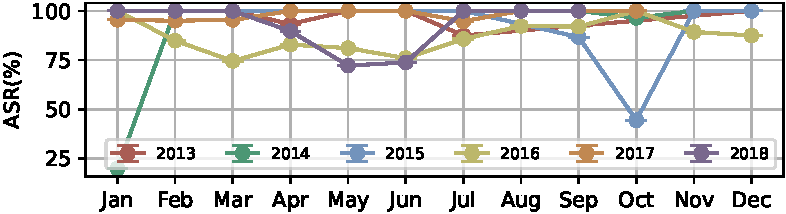
\includegraphics[width=\linewidth,keepaspectratio]{Graph/Evaluation/Figure9.pdf}
	\caption{Attack Persistence over 6 years }
	\label{fig:Attack Persistence-APIGraph}
\end{figure}

The effectiveness of the attack using the problem-space perturbation strategy in poisoned sample generation has already been validated. 
Next, we evaluate the effectiveness of the feature-space perturbation strategy.
We selected 138 families with less than six months of survival for comparative analysis. 
These samples, characterized by their shorter survival times and weaker concept drift attributes, are more suitable for demonstrating the effect of the feature-space perturbation strategy.
We divided the attack targets into five groups based on the duration of the attack test.
The results of the attack  effectiveness are presented in Figure~\ref{fig:feature-space perturbation strategy}.
\begin{figure}[h!]
	\centering
	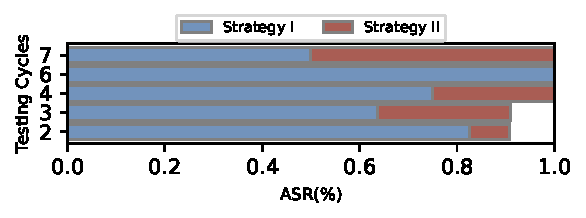
\includegraphics[width=\linewidth,keepaspectratio]{Graph/Evaluation/Figure26.pdf}
	\caption{Feature-space perturbation strategy}
	\label{fig:feature-space perturbation strategy}
\end{figure}
After introducing the SHAP-based feature space perturbation, the attack success rate improved for most targets, reaching an average of 91.3\%.
This represents a 10.9\% increase compared to the previous attack success rate achieved with the problem-space perturbation strategy.
The increase in ASR is due to the attacker  ability to generate poisoned samples with higher uncertainty than those produced using the problem-space perturbation strategy. 
After applying feature-space perturbation, the average uncertainty ranking of the poisoned samples increased by 66.2\%.

Additionally, we further tested the impact on the PACDA when attackers with further limited capabilities as weak Attackers.
First, the attacker cannot query the victim model for sample uncertainty scores. 
In this scenario, the attacker can only obtain the predicted labels from the victim model.
Other information, such as sample uncertainty, must be obtained through the surrogate model.
So we propose a surrogate model construction method based on knowledge distillation, where the surrogate model  parameters $\bm{\theta}_{n-1}^{*}$ approximate those of the victim model $\bm{\theta}_{n-1}$.
\begin{equation}
	\begin{aligned}
			\overline{Y} = Q(\bm{\theta}_{n-1},\bm{D}_{te}^{n-1}) \\
		\end{aligned}
\end{equation}
The attacker constructs a surrogate model $f_{\bm{\theta}_{n-1}^{*}}$ using the input-output query function $Q$, where the pseudo label set $\overline{Y}$ by querying the victim model  $f_{\bm{\theta}_{n-1}}$ with input data $\bm{D}_{te}^{n-1}$.
The purpose of the surrogate model is to identify the optimal parameters $\bm{\theta}_{n-1}^{*}$ such that the prediction error between the surrogate model and the victim model is minimized for all inputs $\bm{\mathrm{x}}_{i} \in \bm{D}_{te}^{n-1}$, as shown in Equation~\ref{Surrogate Model Training}.
\begin{equation}
	\begin{aligned}
			\bm{\theta}_{n-1}^{*} = \arg\min_{\bm{\theta}_{n-2}^{*}} \sum_{\bm{\mathrm{x}_{i}} \in \bm{D}_{te}^{n-1}} \mathcal{L} \left( f_{\bm{\theta}_{n-2}^{*}}(\bm{\mathrm{x}}_{i}) , \overline{y}_{i}  \right),  \overline{y}_{i} \in \overline{Y} \\
		\end{aligned}
	\label{Surrogate Model Training}
\end{equation}
It is important to emphasize that the attacker uses pseudo-labels $\overline{Y}$ generated by the victim model $f_{\bm{\theta}_{n-1}}$ as training labels for the surrogate model rather than relying on ground truth labels.
There are two main reasons for this approach. 
First, the methods of concept drift adaptation are primarily applied in sensitive domains such as malware detection and industrial security risk analysis, where acquiring ground truth labels is prohibitively expensive.
Second, the role of the surrogate model $f_{\bm{\theta}_{n-1}^{*}}$ is to approximate the detection capabilities of the victim model $f_{\bm{\theta}_{n-1}}$, but the victim model does not provide correct labels for the entire testing data $\bm{D}_{te}^{n-1}$. 
As a result, the surrogate model, trained with pseudo-labels, performs more similarly to the victim model.
When constructing the surrogate model $f_{\bm{\theta}_{n-1}^{*}}$, it is important to correctly set the query range for the testing data.
In concept drift cycle $n$, the attacker queries the testing data $\bm{D}_{te}^{n-1}$, which is obtained from the previous concept drift cycle.
This is because the victim model has already completed learning from the previous concept drift cycle.
This model is used to quantify the uncertainty of samples in the current concept drift cycle $n$.
Therefore, to ensure that the surrogate model $f_{\bm{\theta}_{n-1}^{*}}$ approximates the victim model $f_{\bm{\theta}_{n-1}}$, the attacker queries the testing data $\bm{D}_{te}^{n-1}$ and uses the query results to train the surrogate model.

In addition, since computational cost is a primary concern in machine learning scenarios, the attacker  model was weakened to reduce computational overhead.
Specifically, we weaken the model by reducing the number of neural network layers in the encoder or classifier.
Following state-of-the-art Android malware concept drift adaptation methods~\cite{2023-Usenix-chenyizhen}, which employ an encoder and classifier, we tested four weakened settings based on the victim model, as shown in Figure~\ref{fig:Attack-effectiveness-model-heterogeneity}.
ENC denotes the encoder, CAL represents the classifier, and W indicates a decrease in the model  capacity, reflected in a reduction of model parameters.

\begin{figure}[h!]
	\centering
	\includegraphics[width=\linewidth,keepaspectratio]{Graph/Evaluation/Figure10_1.pdf}
	\caption{Attack Effectiveness under Weakened Capabilities}
	\label{fig:Attack-effectiveness-model-heterogeneity}
\end{figure}
\begin{figure*}[t]
	\centering
	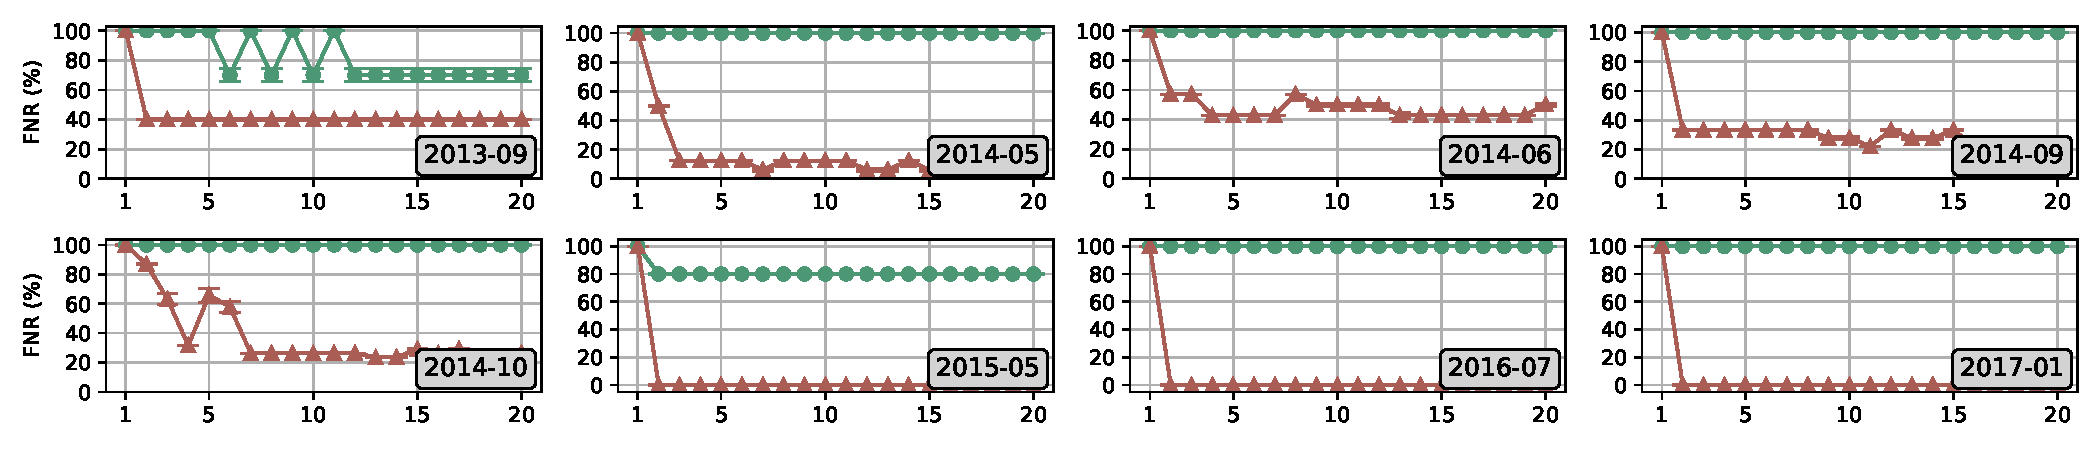
\includegraphics[width=\linewidth,keepaspectratio]{Graph/Evaluation/api_multi_attackers_fnr_1.pdf}
	\caption{Attack Effectiveness with Multi-Target Attack (6 year Attack Testing)}
	\label{fig: Attack Effectiveness with Multi-Target Attack}
\end{figure*}

Previous studies have shown that when the attacker  capabilities are limited, the effectiveness of poisoning attacks decreases~\cite{2022-ACM-Computing-Survey-Threats-to-training}.
However, PACDA mitigates this issue, achieving an average attack success rate of 81.17\% with limited attacker capabilities, as shown in Figure~\ref{fig:Attack-effectiveness-model-heterogeneity}. 
We also found that weakening the encoder reduces the attack success rate by nearly 10\%, which is more significant than weakening the classifier.  
This indicates that the encoder part of the surrogate model plays a crucial role in approximating the capabilities of the victim model.
Additionally, we found that weakening both the encoder and the classifier in the attacker  surrogate model does not result in the lowest attack success rate.
Under this configuration, the attack success rate is even higher than that of the setup where only the classifier is weakened, at 86\% compared to 83\%.
This phenomenon contradicts the expectation that attackers must invest more computational resources to achieve a higher attack success rate.
By analyzing the set of attack targets under different configurations, we found that when the surrogate model is weakened, its selection of attack targets is significantly biased.
In the synchronized weakening setting, only 55\% of the attack targets remain compared to the control group, highlighting the need to assess attack effectiveness under constrained attacker capabilities using ASR and the number of attack targets.
To address this issue, we define the Number of Successful Attack Targets (NSAT) and the Relative Attack Success Rate (RASR), which represents the ratio of successfully attacked targets in the weakened attacker  setup to those in the control group, as shown in Equation~\ref{attack seed formula 1}.
\begin{equation}
	\begin{aligned}
		RASR = \small NSAT_{weak}/\small NSAT_{control}
	\end{aligned}
	\label{attack seed formula 1}
\end{equation}
As model capability weakens, RASR declines, with the weakest setup showing a 43.18\% drop.
While a reduced scope of attack targets weakens the attacker  capabilities, the relative attack success rate increases, posing a significant threat to concept drift adaptation by enhancing resource utilization efficiency even under constrained conditions.

\subsubsection{Multi-Target \DIFaddbegin \DIFadd{(Attacker) }\DIFaddend Attack} 
\label{Sec: Multi Attack Targets}
\DIFaddbegin \DIFadd{As described in Section~\ref{Experimental Setup}, the multi-targets setting simulates two practical scenarios: (1) a single attacker launching attacks against multiple targets, and (2) multiple attackers independently targeting different targets.
For clarity and ease of analysis, we adopt the first scenario, where a single attacker conducts multi-target attacks, as the basis for the following discussion.
}\DIFaddend Multiple attack targets may emerge within the same concept drift cycle in real-world scenarios. 
Therefore, PACDA also supports a multi-target attack mode.
In the multi-target attack setting, the attacker performs PACDA on multiple attack targets simultaneously.
To evaluate the effectiveness of the PACDA in a multi-target setting, we selected 8 months with different attack targets for testing, covering a 6-year evaluation period, as illustrated in Figure~\ref{fig: Attack Effectiveness with Multi-Target Attack}.
For each multi-target setting, we conducted a 20-month attack test.
Detailed information on the settings can be found in Appendix~\ref{Sec: Attack Target List}.
The multi-target attack achieved an average success rate of 97.5\% across different testing times, demonstrating its effectiveness in executing the PACDA on multiple targets.
During the 80-month attack test, only the attack success rate in May 2015 was not 100\%, although it still maintained an effective success rate of 80\%.
The high attack success rate in a multi-target setting is due to the coverage effect of labeling budget consumption across different attack targets.
When multiple attack targets are present, once the labeling budget for the most uncertain attack target is exhausted, the labeling budget for the other attack targets is also concurrently depleted.
Consequently, the PACDA incurs a low cost, as a single attack benefits multiple targets simultaneously.
\DIFaddbegin 

\DIFadd{Then we discuss the scenario where multiple distinct attackers simultaneously target different attack targets.
In terms of attack effectiveness, the success rate in the multi-attacker setting is consistent with that in the single attacker setting with multiple attack targets.
This is because, as previously analyzed, the poisoned samples generated for different attack targets do not interfere with one another.
In fact, poisoned samples crafted for attack targets with the highest uncertainty can even facilitate the misclassification of other attack targets.
Furthermore, we observe that when attack effects are mutually beneficial, attackers tend to cooperate, thereby reducing the overall attack cost. Specifically, multiple attackers can identify the attack target with the highest uncertainty and use it as a common target, allowing them to share the costs involved in poisoned sample generation.
%DIF > 鎺ヤ笅鏉ユ垜浠璁哄涓笉鍚屾敾鍑昏€呭涓嶅悓鏀诲嚮鐩爣鍚屾椂杩涜鏀诲嚮鐨勬儏鍐点€?
%DIF > 鍦ㄦ敾鍑绘晥鏋滄柟闈紝澶氭敾鍑昏€呯殑鏀诲嚮鎴愬姛鐜囦笌鍗曚竴鏀诲嚮鑰呮敾鍑诲涓洰鏍囪缃笅鐨勬敾鍑绘垚鍔熺巼鏄竴鏍风殑銆?
%DIF > 鍥犱负濡備笂杩板垎鏋愭墍绀猴紝閽堝涓嶅悓鏀诲嚮鐩爣鐢熸垚鐨勬姇姣掓牱鏈郊姝や箣闂翠笉浼氫骇鐢熺浉浜掑共鎵帮紝鍙嶈€屾槸鍏锋湁鏈€楂樹笉纭畾鎬х殑鏀诲嚮鐩爣鐢熸垚鐨勬姇姣掓牱鏈彲浠ヨ緟鍔╁叾浠栨敾鍑荤洰鏍囨垚鍔熷疄鐜拌鍒嗙被鐨勬敾鍑绘晥鏋溿€?
%DIF > 骞朵笖鎴戜滑鍙戠幇鍦ㄦ敾鍑绘晥鏋滃彲浠ュ郊姝ゆ敹鐩婄殑鎯呭喌涓嬶紝鏀诲嚮鑰呬箣闂翠細鍊惧悜浜庣浉浜掑悎浣滐紝杩涜€岄檷浣庢暣浣撶殑鏀诲嚮鎴愭湰銆?
%DIF > 鍥犱负澶氫釜涓嶅悓鐨勬敾鍑昏€呭彲浠ラ€夊嚭鏀诲嚮鐩爣涓笉纭畾鎬ф渶楂樼殑鏍锋湰浣滀负缇や綋鏀诲嚮鐩爣锛岃繘鑰屽垎鎽婃姇姣掓牱鏈敓鎴愯繃绋嬩腑鐨勫悇绉嶅紑閿€銆?
}\DIFaddend \begin{table}[h!]
	\caption{Multi-Target Attack across Four Ddatasets}
	\label{tab: asz }
	\setlength{\tabcolsep}{5.8pt}
	\begin{center}
		\scalebox{1.0}{
			\begin{tabular}{ccccc}
				\toprule
				\textbf{Datasets}&\textbf{Targets}&\textbf{F1-Testing} &\textbf{F1-Validation} &\textbf{ASR (\%)} \\
				\midrule
				APIGraph & 734  &  0.76\textsubscript{\textcolor{black}{-0.15}} & 0.99 & 92.92\% \\ 
				\specialrule{0.05em}{1pt}{1pt}
				MNIST & 1,398  & 0.78\textsubscript{\textcolor{black}{-0.12}} & 0.99 & 79.98\%\\
				\specialrule{0.05em}{1pt}{1pt}
				BODMAS & 222  &  0.92\textsubscript{\textcolor{black}{-0.06}}& 0.92 &80.63\% \\ 
				\specialrule{0.05em}{1pt}{1pt}
				SPAM & 168  &  0.91\textsubscript{\textcolor{black}{-0.07}} & 0.99 &74.40\% \\ 
				\bottomrule
		\end{tabular}}
	\end{center}
\end{table}

In certain special cases, the attacker may need to target all attack targets simultaneously.
This represents a special scenario within multi-target attacks.
Therefore, we tested the effectiveness of PACDA on all attack targets at different concept drift time points.
The average attack success rate reaches 81.98\% (as shown in Table~\ref{tab: asz }), with a notably high success rate of 92.92\% achieved on the real-world concept drift dataset, APIGraph.  
Moreover, we observe that the victim models maintain high F1 scores on the initial validation set under attack across different datasets, with an average of 0.99.
This demonstrates that our method preserves the victim model  previously learned knowledge, even when targeting all attack targets, thereby highlighting the stealth of the proposed attack.
The impact on test performance (F1-Testing) varies across datasets, reflecting how limited access to new samples can hinder the model  adaptation to concept drift.
The performance degradation on the BODMAS and SPAM datasets is relatively minor, with average F1-score drops of less than 0.07, indicating a lower intensity of concept drift in these scenarios.
In contrast, the APIGraph and MNIST datasets exhibit more substantial performance changes, with average F1-score drops of around 0.14.
This suggests stronger concept drift and a higher reliance on the victim model for effective learning from drifted samples.
Nevertheless, our attack stealth remains unaffected in both cases, as the testing data is unlabeled, and the victim model cannot promptly detect its performance degradation.

\subsection{Attack Influencing Factors}
\label{Sec: Attack Influencing Factors}

We have demonstrated the effectiveness of PACDA.
To further investigate how real-world conditions affect attack performance, we analyze the factors influencing PACDA using a real-world Android malware dataset (APIGraph~\cite{2020-CCS-APIGraph}) spanning seven years.

\subsubsection{Impact of Different CDA-AL Strategies}
Existing concept drift adaptation strategies in sensitive domains~\cite{2023-Usenix-chenyizhen,2022-SP-Trancending,2021-Usenix-CDAE} can be broadly categorized into four types. 
In addition to the uncertainty-based strategies discussed in Section~\ref{Sec: Concept Drift Adaptation}, the remaining approaches fall into three categories. 
To ensure the generality of our findings, we evaluate the effectiveness of our attack across all these representative adaptation strategies.

\begin{itemize}[leftmargin=0.35cm]

\item CADE~\cite{2021-Usenix-CDAE} trains an encoder with labeled data to learn compressed input representations. 
It uses a distance function to identify concept drift samples that deviate from the training data.
\begin{equation}
	\begin{aligned}
		d_{i} = ||\bm{\mathrm{z}}_{i}-\bm{\mathrm{zc}}_{i}||_{2} \\
	\end{aligned}
	\label{CADE}
\end{equation}
Specifically, $\bm{\mathrm{z}}_{i}$ represents the latent space embedding of the sample $\bm{\mathrm{x}}_{i}$ obtained from the encoder. 
A sample is a concept drift instance if its distance $d_{i}$ to the nearest training sample in the encoder  latent space exceeds a predefined threshold.
\item TRANS~\cite{2022-SP-Trancending}
applies conformal prediction~\cite{2005-high-cite-Algorithmic-learning-in-a-random-world} to concept drift adaptation.
It calculates a testing sample  non-conformity score, credibility (proportion of calibration samples with higher scores), and confidence (1 minus the opposite label  credibility). 
Low scores indicate potential drift.
\item HCL~\cite{2023-Usenix-chenyizhen}
proposes the latest concept drift adaptation strategy, combining an encoder and classifier. 
Its training loss $\mathcal{L}(\bm{\mathrm{x}}_{i})$ integrates hierarchical contrast loss $\mathcal{L}_{hc}(\bm{\mathrm{x}}_{i})$ and classification loss $\mathcal{L}_{ce}(\bm{\mathrm{x}}_{i})$.
\begin{equation}
	\begin{aligned}
		\mathcal{L}(\bm{\mathrm{x}}_{i}) = \mathcal{L}_{hc}(\bm{\mathrm{x}}_{i}) + \mathcal{L}_{ce}(\bm{\mathrm{x}}_{i}) \\
	\end{aligned}
	\label{CADE}
\end{equation}
Samples with higher loss values are more likely to be affected by concept drift, as different samples incur different loss levels during inference.

\end{itemize}
%The evaluation includes both traditional model uncertainty approaches and concept drift adaptation strategies that leverage advanced machine learning techniques, such as contrastive learning.
%As shown in Figure~\ref{fig:Attack-effectiveness-Concept-Drift-Strategy}, the experimental results demonstrate that our attack consistently achieves an attack success rate exceeding 80\% across four various concept drift adaptation strategies.
%Furthermore, during the attack process, the performance metrics of the primary task remain stable, with the F1 consistently exceeding 0.88 across all strategies.
%Notably, the ASR reaches 92.77\% when targeting the currently optimal concept drift adaptation method (HCL).
%The primary reason PACDA achieves the highest attack success rate on HCL is that HCL selects concept drift samples based on their loss function values, making the constructed poisoned samples significantly impact the retraining process of the victim model.
%As a result, ensuring the security of concept drift adaptation methods has become an urgent challenge requiring immediate attention.
% Version
%The evaluation includes traditional uncertainty-based approaches and advanced concept drift adaptation strategies, such as contrastive learning.
%As shown in Figure~\ref{fig:Attack-effectiveness-Concept-Drift-Strategy}, PACDA achieves an ASR exceeding 80\% across all four strategies while maintaining stable primary task performance, with F1 consistently above 0.88.
%Notably, PACDA achieves a 92.77\% ASR against the optimal concept drift adaptation method (HCL).
\begin{figure}[h!]
	\centering
	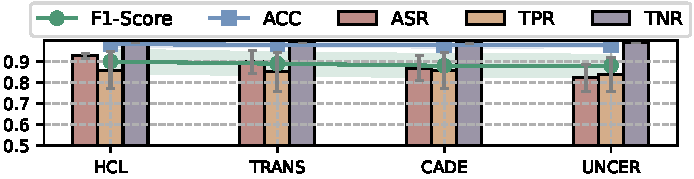
\includegraphics[width=\linewidth,keepaspectratio]{Graph/Evaluation/Figure13.pdf}
	\caption{Different Concept Drift Adaptation Strategies}
	\label{fig:Attack-effectiveness-Concept-Drift-Strategy}
\end{figure}
The evaluation covers traditional uncertainty-based methods and advanced concept drift strategies like contrastive learning.
As shown in Figure~\ref{fig:Attack-effectiveness-Concept-Drift-Strategy}, PACDA achieves over 80\% ASR across all four strategies while maintaining F1 scores above 0.88.
PACDA attains a 92.77\% ASR against the latest adaptation method (HCL).
%These results highlight the urgent need to address security challenges in concept drift adaptation methods.

%\begin{figure}[h!]
%	%\vspace{-0.8em}
%	\centering
%	\subfloat[Different Strategies]{
%		\label{fig11-1}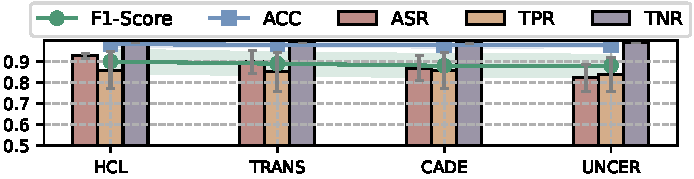
\includegraphics[width=4.25cm, height=2.9cm]{Graph/Evaluation/Figure13.pdf}
%	}
%	\subfloat[Labeling Budget]{
%		\label{fig11-2}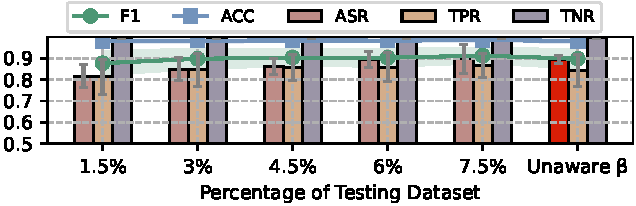
\includegraphics[width=4.25cm, height=2.9cm]{Graph/Evaluation/Figure14_3.pdf}
%	}
%	\caption{xxxxxxxxxxxxx.} 
%	\label{fig111}
%	%\vspace{-1em}
%\end{figure}

\subsubsection{Impact of Labeling Budget}
\label{Sec: Attack Effectiveness under Different Label budget}
The labeling budget represents the cost of manual labeling and is one of the most valuable resources in CDA-AL.
We evaluated the attack effectiveness under six different labeling budget settings.
Each labeling budget setting represents its proportion of the testing data, following the settings of existing studies~\cite{2023-Usenix-chenyizhen}.
The first five labeling budget settings assume the attacker knows the victim model  labeling budget.
In contrast, the last setting assumes the attacker cannot access the victim model  labeling budget.
When the attacker is unaware of the labeling budget settings, poisoned samples are generated based on the maximum computational capacity of the attacker. 
In this experiment, we set the attacker  capacity four times the potential labeling budget computation capacity.
\begin{figure}[h!]
	\centering
	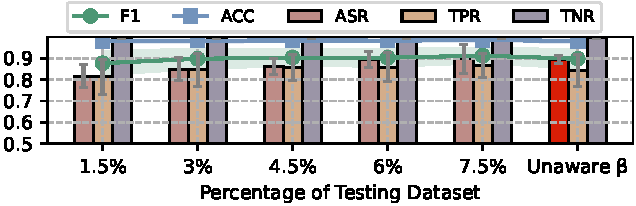
\includegraphics[width=\linewidth,keepaspectratio]{Graph/Evaluation/Figure14_3.pdf}
	\caption{PACDA Under Different Labeling Budget}
	\label{fig:Attack-effectiveness-Label-Budget}
\end{figure}
As shown in Figure~\ref{fig:Attack-effectiveness-Label-Budget}, PACDA remains effective across budgets, with an average attack success rate of 86.30\%.
Even without access to the victim model  labeling budget, the attacker can still achieve a high attack success rate by leveraging the maximum available resources, reaching 89.33\%.
The high attack success rate, even without access to detailed labeling budget information, is due to the significantly lower cost of poisoning attacks than the victim  concept drift adaptation cost, which is primarily driven by labeling expenses.
Thus, the attacker can generate as many poisoned samples as possible to consume the victim model  labeling budget.
This strategy is inspired by DDoS~\cite{mirkovic2004taxonomy} attacks, where the attacker maximizes attack traffic without knowing the victim  total resources to achieve the attack objective.
\DIFaddbegin \DIFadd{Moreover, even if the scale of poisoned samples in the PACDA attack exceeds the labeling budget, it is unlikely to raise suspicion.
This is because the poisoned samples are injected into the unlabeled testing data stream during each concept drift cycle, and the volume of this stream is substantially larger than the victim model  monthly labeling budget.
As a result, PACDA exhibits strong stealth. 
Furthermore, it is extremely difficult for the victim model to detect poisoned samples within the testing data stream due to the massive volume of incoming data, which makes full inspection infeasible.
}

\DIFaddend %In our setup, the label budget reflects a victim model  real-world capabilities.\footnote{According to Kaspersky  2023 statistics~\cite{Kaspersky-Android-Malware-Threat-Statistics}, the total number of Android malware samples for the year reached 1.12 million. Using the commonly assumed 9:1 ratio of benign to malicious samples, the total number of benign and newly detected malicious samples per month is estimated to be 11.2 million.}
%The maximum budget of 300 samples represents approximately 9\% of the monthly test data, which is equivalent to the manual analysis of 83,761 samples each month in real-world scenarios.
%An estimated cost of 22 USD per sample (obtained through interviews with security vendors) translates to 1.84 million USD per month, representing a substantial financial burden for security companies.

%\subsubsection{Impact of Data Collection Capability}
%In multi-target attacks, there is a special case where the attack target consists of all the test data.
%In this case, the attacker  poisoning seed samples need to be the highest uncertainty samples from the test dataset, making data collection capability crucial to its effectiveness.
%So we conducted attack experiments with five settings on four datasets.
%PACDA relies on identifying high-uncertainty attack seeds to generate poisoned samples.
%The uncertainty of these seeds is influenced by the attacker  data collection capabilities, affecting the overall attack effectiveness.
%Tests were conducted across four datasets under different data collection capacities to analyze their effects on attack performance, as illustrated in Figure~\ref{fig:Impact of Data Collection Ability}.
%\begin{figure}[t]
%	\centering
%	\includegraphics[width=\linewidth,keepaspectratio]{Graph/Evaluation/figure17-v3.pdf}
%	\caption{Impact of Data Collection Ability}
%	\label{fig:Impact of Data Collection Ability}
%\end{figure}
%No clear correlation was observed between reduced data collection capability and diminished attack effectiveness.
%Across all four datasets, reduced data collection sometimes improved attack performance. 
%For instance, in the MNIST dataset, attacks with 90\% data collection capability outperformed those with 100\% capability in over 80\% of the attack test cycles.
%Similarly, in the APIGraph~\cite{2020-CCS-APIGraph} dataset, 50\% capability occasionally surpassed 100\% in specific periods.
%The above analysis shows that attack effectiveness relies more on the presence of high-uncertainty samples than on data collection capability alone.
%Even when there are differences in data quantity and distribution between the attacker and the victim model, attackers can still achieve significant success by acquiring such samples.

\subsubsection{Impact of Attack Value Assessment}
Analyzing the attack value of attack targets provides crucial support for the PACDA.
To demonstrate the significance of this step, we conduct ablation experiments where attackers skip the attack value assessment phase and proceed directly to poisoning seed sample selection and poisoned sample generation.
This approach implies that attackers target all new malware, leading to a significant increase in attack cost.
%\begin{table}[h]
%	\centering
%	%	\renewcommand{\arraystretch}{0.9}  % 璋冩暣琛ㄦ牸鐨勮璺?
%	\small
%	\caption{Attack value assessment necessity analysis}
%	\label{tab: Attack Value Assessment necessity analysis}
%	%\renewcommand{\arraystretch}{0.75}  % 璋冩暣璇ヨ〃鏍肩殑琛岃窛
%	\begin{tabular}{ccc}
%		\toprule
%		% \textbf{Setting} & \textbf{Ablation-ASR} & \textbf{ASR} & \textbf{Improvement} & \textbf{Sample Reduction} \\
%		\textbf{Stratege} & \textbf{Ablation-ASR (\%)} & \textbf{ASR (\%)}\\
%		\midrule
%		HCL (Model Based) & 81.73 & \textbf{92.77}\textsubscript{\textcolor{red}{\textbf{+11.04}}}\\
%		CADE (Data Based) & 72.43 & \textbf{86.90}\textsubscript{\textcolor{red}{\textbf{+14.47}}}\\
%		%UNCER & 61.50 & \textbf{82.86}\textsubscript{\textcolor{red}{\textbf{+21.36}}}\\
%		\bottomrule
%	\end{tabular}
%\end{table}
\begin{table}[h!]
	\caption{Attack value assessment necessity analysis}
	\label{tab: Attack Value Assessment necessity analysis}
	\setlength{\tabcolsep}{5.8pt}
	\begin{center}
		\scalebox{1.0}{
			\begin{tabular}{ccc}
				\toprule
				\textbf{CDA-AL Strategies}&\textbf{Ablation-ASR (\%)}&\textbf{ASR (\%)} \\
				\midrule
				HCL (Model Based) & 81.73  &  92.77\textsubscript{\textcolor{red}{+11.04}} \\ 
				\specialrule{0.05em}{1pt}{1pt}
				CADE (Data Based) & 72.43  & 86.90\textsubscript{\textcolor{red}{+14.47}} \\
				\bottomrule
		\end{tabular}}
	\end{center}
\end{table}

Existing concept drift adaptation strategies are primarily divided into data-driven and model-driven approaches.
Therefore, in the attack value assessment module, we selected two representative strategies, CADE and HCL, from each category for evaluation. 
For the labeling budget, we chose a medium-level sample labeling capacity and set the labeling budget to 200.
The experimental results reveal that removing the attack value assessment module leads to an average decrease of 15.62\% in attack success rates, as shown in Table~\ref{tab: Attack Value Assessment necessity analysis}.
This highlights the critical role of the attack value assessment module in PACDA.

		\section{Potential Defenses}
\label{Sec: Potential Defenses}
CDA-AL methods lack directly relevant and effective defenses against poisoning attacks.
While Lin et al.~\cite{2021-GLOBALCOM-acctive-learning-under-malicious-mislabeling-poisoning-attacks} proposed defenses for active learning poisoning attacks based on static unlabeled and clean datasets. 
However, these assumptions break down in CDA-AL, where unlabeled data evolves and clean datasets quickly become outdated.
Therefore, we evaluated PACDA against four representative poisoning attack defense mechanisms~\cite{AC,DFP,FT,FP}.
\begin{itemize}[leftmargin=0.35cm] % 鑷畾涔夌缉杩?
	\item \textbf{Activation Clustering (AC)}~\cite{AC} is a data inspection method that assumes poisoned data forms a distinct cluster within the target class, either small or distant from the class center. 

	\item \textbf{Data-Free Pruning (DFP)}~\cite{DFP} sanitizes poisoned models by pruning neurons dormant for clean data, assuming poisoned and clean data activate different neurons.

	\item \textbf{Fine-Tuning (FT)}~\cite{FT} can mitigate targeted poisoning attacks, but it requires extensive labeled training data to avoid overfitting.

	\item  \textbf{Fine-Pruning (FP)}~\cite{FP} mitigates poisoned models by pruning neurons dormant on clean validation data, measuring average neuron activation, and removing the least active ones. 
\end{itemize}
%\begin{table}[t]
%	\caption{Existing Defenses Against PACDA} %鏍囬
%	\label{tab: Analysis of Existing Defenses Against Poisoning Attacks (TPA)} %琛ㄦ爣绛?
%	\centering
%	\renewcommand{\arraystretch}{0.9}  % 璋冩暣琛ㄦ牸鐨勮璺?
%	\small
%	\begin{tabular}{|c|c|c|}
%		\hline
%		\textbf{Method}  & \textbf{F1-score} & \textbf{Avarage ASR Decrease (268 Months)}  \\ \hline
%		AC~\cite{AC} & 0.90 &  16.5\%\\ \hline
%		DFP~\cite{DFP}   & 0.87 & 21.8\%  \\ \hline
%		FT~\cite{FT}   & - & without extensive labeled training dataset   \\ \hline
%		FP~\cite{FP}   & - & without clean labeled validation dataset   \\ \hline
%		ICDF(Our) & 0.90 &  \textbf{39\%}  \\ \hline
%	\end{tabular}
%\end{table}

The defense assumptions of FT and FP rely on the victim model having access to a large amount of labeled clean data for fine-tuning or model pruning.
However, this assumption is impractical in concept drift adaptation scenarios, where the labeling budget is limited each month, and the training data distribution is continuously evolving.
Therefore, the FT and FP methods cannot be executed under the active learning-based concept drift adaptation setting.
Under this setting, defenses based on feature separability (AC) and model parameter adjustments (DFP) are applicable, but their defensive effectiveness is limited.
As shown in Figure~\ref{fig:ICDF Defense Motivation}, t-SNE
visualization reveals that PACDA  use of attack seeds creates intricate entanglement between poisoned and clean samples in the
feature space (the APIGraph dataset  test data from June 2013).
\DIFdelbegin \DIFdel{Consequently, existing defences perform poorly, failing to remove
poisoned samples}\DIFdelend \DIFaddbegin \DIFadd{As a result, existing defenses cannot distinguish between clean and poisoned samples, so they cannot fully defend against PACDA attacks}\DIFaddend .
\begin{figure}[h!]
	\centering
	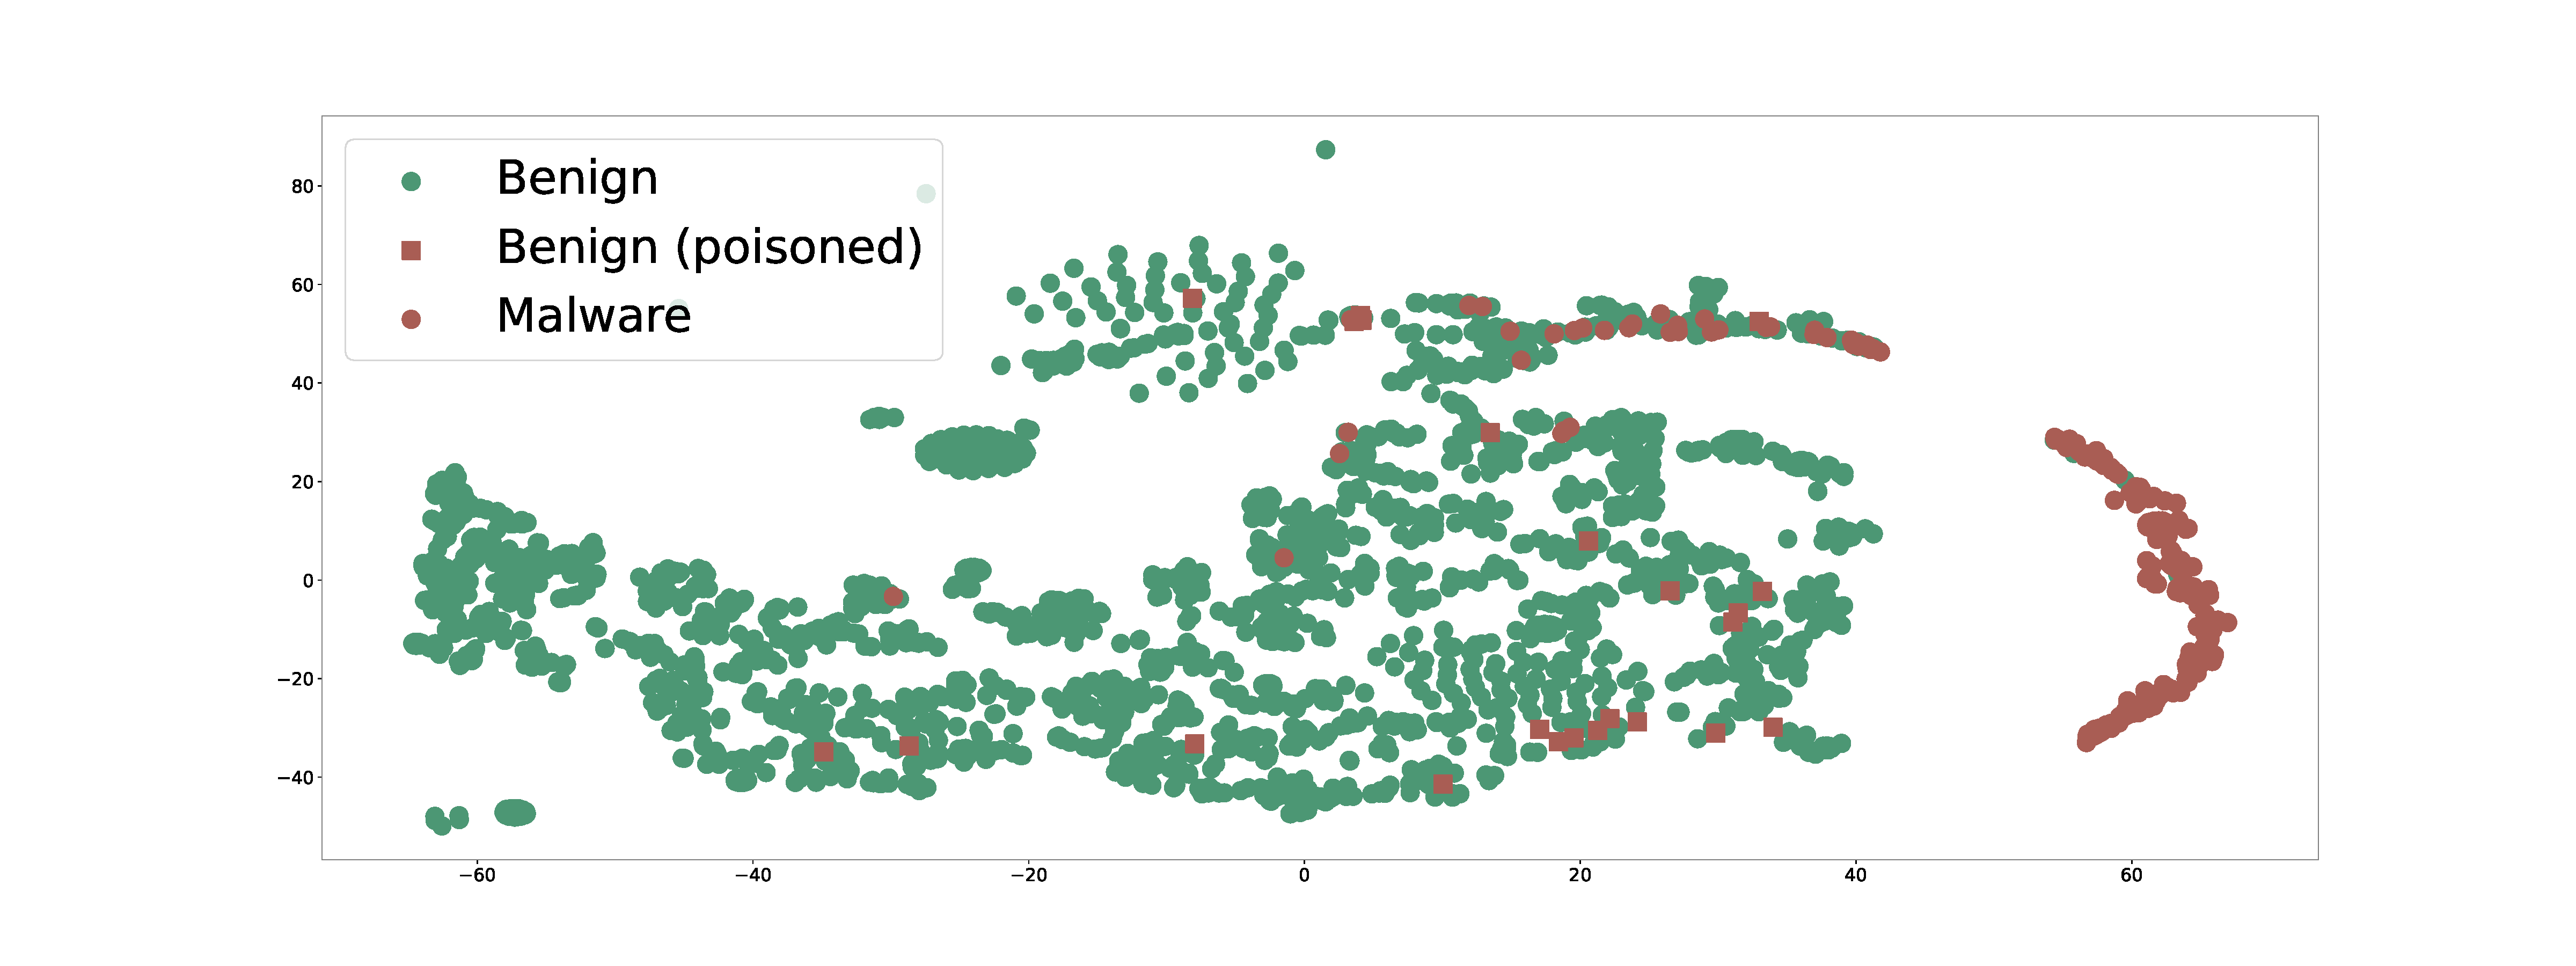
\includegraphics[width=\linewidth,keepaspectratio]{Graph/Evaluation/Figure20.pdf}
	\caption{ICDF Defense Motivation}
	\label{fig:ICDF Defense Motivation}
\end{figure}
Thus, the attack success rate decreases by less than 20\% on average. Specifically, the ASR drops by 16.5\% under the AC defense and 21.8\% under DFP.
Given these limitations, we explore alternative defense strategies in countering PACDA.

Intra-Cluster Distance Filtering (ICDF): In the PACDA, the attacker relies on poisoning seed samples to generate poisoned samples, reducing costs and leading to similarity among the poisoned samples.
Different poisoned samples may originate from the same seed sample.
We measure this similarity using Euclidean distance in the feature space, the basis for our defense method (ICDF).
Unlike AC-based defenses, ICDF filters poisoned samples by exploiting the similarities between the poisoned samples themselves.
%Motivated by this observation, we propose an adaptive sample filtering method based on intra-cluster distance.
%Unsupervised clustering algorithms (e.g., K-means) are applied to the concept drift samples, partitioning the data into $\mathcal{C}$ clusters.
%Each cluster $c \in \mathcal{C}$ contains multiple concept drift samples, and the intra-cluster distance threshold $\tau$ is determined by calculating the mean Euclidean distance between any two samples within the same cluster.
%For each cluster $c$, samples with distances to other samples smaller than the cluster-specific threshold $\tau$ are removed.
So, we propose an adaptive sample filtering method based on intra-cluster distance.
Specifically, using an unsupervised clustering algorithm (e.g., K-means), we partition the concept drift samples into a set of clusters $Clu$ ($Clu= \{c_{1},c_{2},..,c_{k} \}$).
Each cluster $c_{k}$ calculates an intra-cluster distance threshold $\tau$ (Equation~\ref{ICDF Defense Method}) as the mean Euclidean distance $d_{Euc}(\bm{\mathrm{x}}_{i}, \bm{\mathrm{x}}_{j})$ between its samples.
\begin{equation}
	\begin{aligned}
		\tau = \frac{1}{|c_{i}| (|c_{i}| - 1)} \sum_{i \neq j} d_{Euc}(\bm{\mathrm{x}}_{i}, \bm{\mathrm{x}}_{j}) \quad i,j \in c_{k}
	\end{aligned}
	\label{ICDF Defense Method}
\end{equation}
$|c_{i}|$ is the number of samples in the cluster $c_{i}$.
Samples with distances smaller than $\tau$ to others in the same cluster are removed.
%\begin{figure}[t]
%	\centering
%	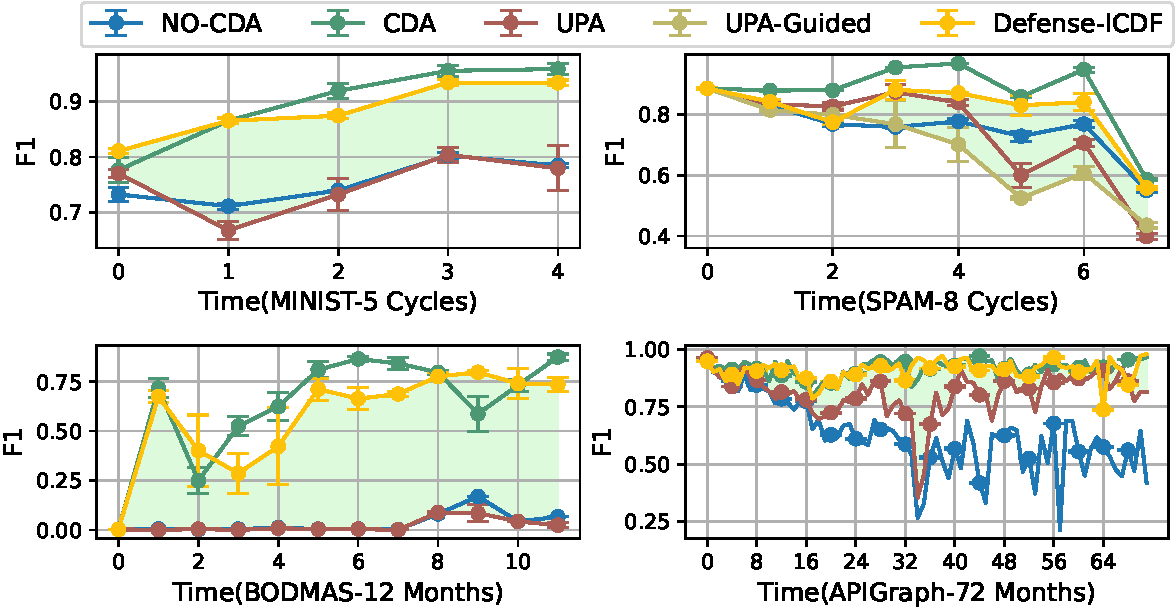
\includegraphics[width=\linewidth,keepaspectratio]{Graph/Evaluation/Figure19_1.pdf}
%	\caption{ICDF Defense (Multi-Target PACDA)}
%	\label{fig:ICDF Defense against Untargeted Poisoning Attack}
%\end{figure}
%\begin{figure}[h!]
%	%\vspace{-0.8em}
%	\centering
%	\subfloat[ICDF Defense Single-Target]{
%		\label{fig11-1}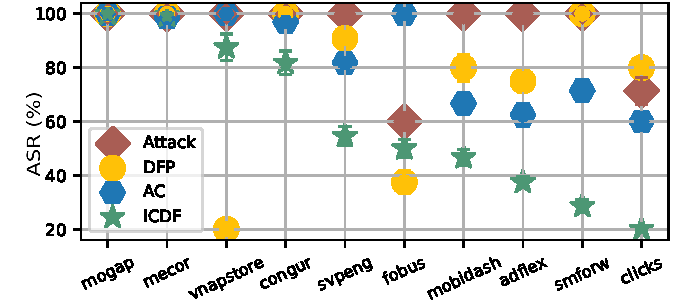
\includegraphics[width=3.90cm, height=2.9cm]{Graph/Evaluation/Figure-last_1.pdf}
%	}
%	\subfloat[ICDF Defense Multi-Target ]{
%		\label{fig11-2}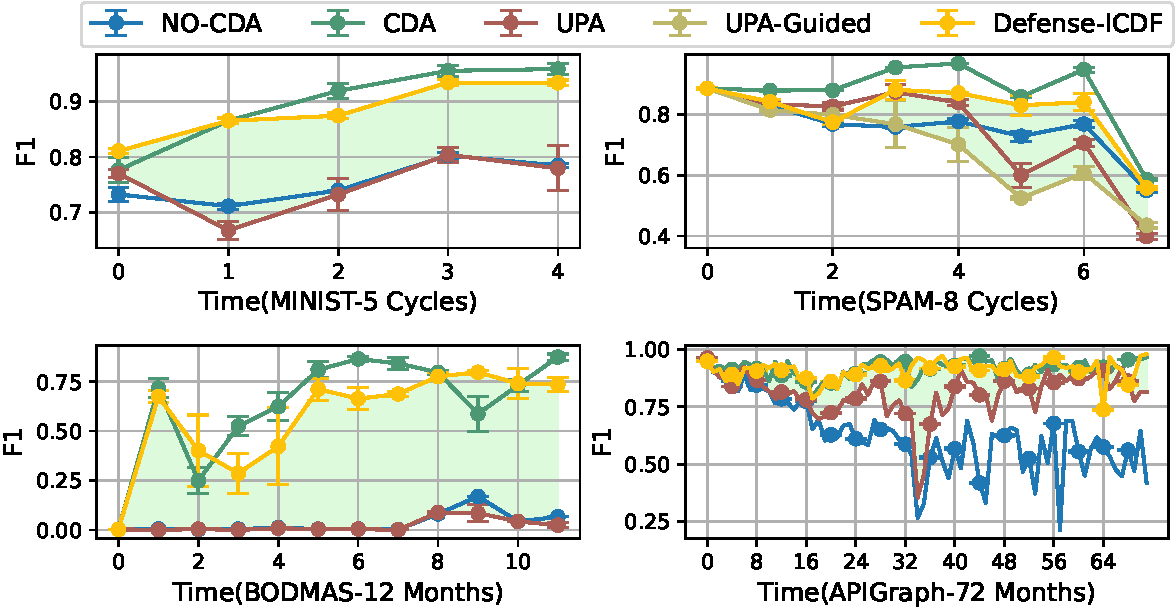
\includegraphics[width=4.60cm, height=2.9cm]{Graph/Evaluation/Figure19_1.pdf}
%	}
%	\caption{xxxxxxxxxxxxx.} 
%	\label{fig111}
%	%\vspace{-1em}
%\end{figure}
%The defense effectiveness against UPA is shown in Figure~\ref{fig:ICDF Defense against Untargeted Poisoning Attack}, demonstrating that the proposed defense method is effective across all four datasets.  
%For clarity, we used green shading to indicate the portion of model performance improvement after applying the ICDF defense method compared to the model performance under attack.
%Notably, in the MNIST and BODMAS datasets, the model performance during certain testing periods even exceeded the optimal performance of concept drift adaptation.  
%This demonstrates that our defense method not only filters out poisoned samples but also enhances the performance of concept drift adaptation itself.
%Among the datasets, the BODMAS dataset exhibited the greatest improvement, with an average F1 increase of 0.52 and a maximum increase of 0.78.
%\textbf{The ICDF defence effectively counters multi-target attack across all four datasets.}
%Green shading highlights performance improvements after applying ICDF, with notable gains in MNIST and BODMAS, where model performance during some periods surpassed the optimal performance of concept drift adaptation.
%The superior performance over the best original concept drift adaptation is due to ICDF's clustering approach, which removes poisoned samples and reduces data redundancy in clean samples, improving training efficiency.
%Although there is a lack of research in the concept drift field, studies in computer vision have shown that data redundancy reduces model training efficiency~\cite{kong2023peeling}.
%Since improving concept drift adaptation is beyond the scope of this study, we will address it in future research.
\begin{figure}[h!]
	\centering
	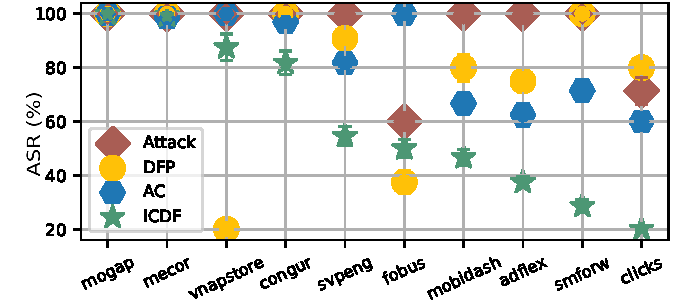
\includegraphics[keepaspectratio,height=3.5cm]{Graph/Evaluation/Figure-last_1.pdf}
	\caption{ICDF Defense (Single-Target PACDA)}
	\label{fig:APIGraph-targeted-defense}
\end{figure}
ICDF achieved the best defense effect under single-target attack mode, reducing the success rate of PACDA by 39\% across the Top 10 target sets, as shown in Figure~\ref{fig:APIGraph-targeted-defense}. 
While AC and DFP showed some effectiveness, they were 23.5\% and 18.8\% less effective than ICDF.
We also evaluated our method's defense performance against feature space ased poisoned sample generation strategies on the APIGraph dataset. 
The attack success rate was reduced by 32.6\%, under the same experimental settings as those used in the attack effectiveness evaluation.
We also conducted defense tests against multi-target attacks across four different datasets, as shown in Table~\ref{tab:dma }.
The attack success rate decreased by an average of 54.97\% across the four datasets\DIFdelbegin \DIFdel{, while the F1 score on the mapping dataset was restored to an average of 0.91}\DIFdelend .
Therefore, our ICDF defense method also demonstrates strong effectiveness in defending against multi-target attack scenarios.
\DIFaddbegin \DIFadd{Moreover, after introducing the ICDF defense method, the F1 score on the four datasets was restored to an average of 0.91, indicating that the normal concept drift adaptation performance was not affected.
}\DIFaddend \begin{table}[h!]
	\caption{ICDF Defense (Multi-Target PACDA)}
	\label{tab:dma }
	\setlength{\tabcolsep}{5.8pt}
	\begin{center}
		\scalebox{1.0}{
			\begin{tabular}{ccccc}
				\toprule
				\textbf{Datasets}&\textbf{Targets}&\textbf{F1-Attack} &\textbf{F1-Defense} &\textbf{ASR-Decrease} \\
				\midrule
				APIGraph & 734  &  0.76 & 0.90\textsubscript{\textcolor{red}{\textbf{+0.14}}} & 21.26\% \\ 
				\specialrule{0.05em}{1pt}{1pt}
				MNIST & 1,398  & 0.78 & 0.82 \textsubscript{\textcolor{red}{\textbf{+0.04}}}& 75.47\%\\
				\specialrule{0.05em}{1pt}{1pt}
				BODMAS & 222  &  0.92 & 0.99\textsubscript{\textcolor{red}{\textbf{+0.07}}} &54.05\% \\ 
				\specialrule{0.05em}{1pt}{1pt}
				SPAM & 168  &  0.91 & 0.94\textsubscript{\textcolor{red}{\textbf{+0.03}}} &69.04\% \\ 
				\bottomrule
		\end{tabular}}
	\end{center}
\end{table}

To better demonstrate the effectiveness of the ICDF method, we analyze the variation in defense performance under different parameter settings.
We selected the APIGraph dataset, which spans the longest time period, for defense parameter analysis.
The number of clusters was the only parameter requiring manual configuration during the defense.
We conducted analyses under both single-target and multi-target attack scenarios.  
We evaluated four cluster settings (6, 10, 20, and 40) under the multi-target attack. 
The mean F1 score across these four settings was 0.91, with a variance of 0.0025.
Given the large number of attack targets in the single-target setting, we selected a subset of representative malware families for detailed evaluation.
In the single-target attack, we selected the family 'clicks' (with the best ICDF defense performance) and the family 'mogap' (with the worst ICDF defense performance) from the Top 10 attack targets.
For each family, we conducted four experiments with clustering parameter settings of 6, 10, 20, and 40 and observed that the defense performance remained consistent across all settings.
This indicates that the defense parameter settings have minimal impact on defense effectiveness, which can effectively reduce the deployment costs of the defense method.

		%\section{Future Work and Conclusion}
%%%%%%%%%%%%%%%%%%%%%%2025-Usenix-鎶曠鎷掔粷鐗堟湰%%%%%%%%%%%%%%%%%%%%%%%%
%\noindent In this study, we introduce an efficient framework for poisoning attack against concept drift adaptation (PACDA). 
%In the following, we discuss some limitations of our attack method and outline potential future research directions.
%
%%\textcolor{blue}{Although PACDA may not extensively search for poisoning seed samples, we have multiple attack strategies to choose from, which do not compromise the overall attack effectiveness.}
%
%\textbf{Limitation of PACDA}: In the process of PACDA, it is necessary to rely on poisoned seed samples with high uncertainty scores. 
%However, in some cases, such high uncertainty score samples may not appear in the test dataset of the current month or the attack value of new malware samples is unstable. 
%To enable PACDA to adapt to such scenarios, we adopt strategies to relax the uncertainty score constraints or employ a freeze attack strategy.
%Refer to Appendix \ref{Sec: Attack Value Unstable} for details about attack value unstable and freeze attack.
%%Freeze attack strategy can effectively help us to solve the problem of inability to obtain attack seed samples. 
%Nevertheless, we acknowledge that freeze attack may potentially reduce the success rate or stealthiness of the attack. 
%In future research, we plan to overcome these limitation.
%
%%\textcolor{blue}{Currently, there is a lack of defense methods against PACDA. In the future, research could consider starting with the detection of poisoning samples.}
%
%%\textcolor{blue}{Our attack is versatile, so in the future, we plan to construct more concept drift datasets to verify the effectiveness of the attack.}
%
%\textbf{More Datasets for Validation}: In this research, we primarily concentrate on validating the effectiveness of our attacks using concept drift datasets of Android malware.
%%The primary reason for this focus lies in the fact that currently, publicly accessible concept drift datasets in the security domain are predominantly centered around Android malware.
%However, our PACDA has universal applicability to concept drift adaptation.
%In the future, we aim to collaborate with security vendors to gather additional malicious objects from various scenarios, including spam detection, malicious PDF identification, and Windows malware detection. This will enable us to construct a more diverse and comprehensive concept drift dataset, and subsequently validate the effectiveness of our PACDA.
%%%%%%%%%%%%%%%%%%%%%%2025-Usenix-鎶曠鎷掔粷鐗堟湰%%%%%%%%%%%%%%%%%%%%%%%%

%%%%%%%%%%%%%%%%%%%%%%2025-CCS-鎶曠鐗堟湰%%%%%%%%%%%%%%%%%%%%%%%%
%\subsection{Future Work}
%In this study, we introduce an efficient framework for poisoning attack against concept drift adaptation (PACDA). 
%In the following, we discuss the limitations of this work and point to several future directions.

%\noindent \textbf{(i) Dependency to Attack Seed Samples:} 
%The effectiveness of our attack demonstrates that searching for attack seed samples is a viable approach, and modifying samples can effectively alter their uncertainty scores, as illustrated in Figure~\ref{fig:Case Study of Uncertainty Dynamics}. However, PACDA still relies on attack seed samples to reduce attack costs. In future work, we aim to eliminate this dependency and explore seed-free approaches.

% 杩欒瘽涓嶈浜嗭紝璇翠簡娌″噯琚綋浣滃绋挎剰瑙?
%Specifically, precise handling of sample uncertainty in sensitive domain data will be a critical focus of our research.
%\noindent \textbf{(i) Optimal Defenses Parameters:} 
%We have successfully implemented effective defenses against the PACDA, further research could focus on enhancing the model's concept drift adaptation performance while simultaneously mitigating the attack success rate.
%Moreover, during the defender's unsupervised clustering process, the number of clusters must be specified as a defense parameter. 
%While different numbers of clusters correspond to varying levels of defense strength, future research could explore adaptive methods for setting defense parameters.
%A future direction is to explore efficient techniques to compute the optimal defense parameters.
%We have implemented effective defenses against the PACDA, future research could focus on improving concept drift adaptation performance while reducing the impact of attacks.
%Additionally, in the defender's unsupervised clustering process, specifying the number of clusters is a key defense parameter. 
%Since varying cluster numbers impact defense strength, future work could explore adaptive methods to compute optimal defense parameters at different time.\
%\noindent \textbf{(i) Generalization to Continual Learning:} 
%Although this study primarily focuses on the security of concept drift adaptation methods, we plan to extend our research to address the security challenges associated with continual learning in future work. 
%Concept drift adaptation primarily addresses the challenge of evolving data distributions within a single task over time, while continual learning focuses on sequentially learning across multiple tasks. 
%Despite their differences in the types of learning tasks they target, both approaches aim to tackle the challenges posed by the dynamic and ever-changing data environments of the real world.
%Our study focuses on the security of concept drift adaptation methods, future work we want to study security challenges in continual learning.
%While concept drift adaptation handles evolving data distributions within a single task, continual learning addresses sequential learning across multiple tasks.
%Despite these differences, both approaches aim to address the challenges of dynamic and ever-changing real-world data environments.
%This study focuses on the security of concept drift adaptation methods based on active learning.
%In future work, we aim to extend our research to the security of continual learning, as both learning paradigms are designed to address the challenges posed by dynamic and ever-changing real-world data environments.
%The continuous changes in real-world environments also present opportunities for attackers.
% 杩欎釜涓句緥涓嶈浜嗭紝鍏嶅緱瀹$浜洪『鐫€闂嚭闂鏉?
%For instance, in the context of malware detection, a binary classification task on the same dataset falls within the research area of concept drift adaptation.
%In contrast, a multi-class classification task for malware families aligns with the domain of continual learning, as new malware families continuously emerge.
%\noindent \textbf{(ii) More Real-World Concept Drift Datasets:} 
%Although research on concept drift detection and adaptation has advanced rapidly in recent years, most existing concept drift datasets are either synthesized from pre-existing datasets or have a limited time span, making them unsuitable for long-term concept drift studies.
%Therefore, we plan to further collect more real-world concept drift datasets in the future to facilitate the advancement of research in this area.
%We aim to make further contributions to the model security research community.
%While concept drift research has advanced, most datasets are synthetic or have limited time spans. 
%In the future, our work will focus on collecting more long-term concept drift datasets from the real world.
%In industrial risk control, concept drift datasets are crucial as they directly affect physical safety.
%\noindent \textbf{(ii) Robust Active Learning FrameWork:} 
%The proposed defense method introduces a security component to existing CDA-AL approaches, resulting in increased computational costs. 
%Future research will explore integrating poisoned sample filtering into the concept drift sample selection process, aiming to further reduce the cost of PACDA defenses.
%Our defence method adds a security component to CDA-AL, increasing computational costs.
%Future work will integrate poisoned sample filtering with concept drift sample selection to reduce PACDA defence costs and improve adaptation performance.

\section{Limitation and Discussion}

\subsection{Existence of Attack Seeds}
Our attack relies on poisoning seeds to craft effective poisoned samples.
Experiments across four datasets show that suitable seeds can be identified for most targets.
We also consider extreme cases with no seeds, such as when the attack target is the most uncertain sample in the testing data.
In such cases, attackers can delay releasing the attack target and wait for the next concept drift cycle to obtain viable seeds, as long-term misclassification holds more value than immediate impact.
Moreover, by leveraging SHAP-based feature space perturbation, we can elevate the uncertainty of less uncertain samples and use them as substitute seeds. 
Thus, PACDA remains feasible even when seeds are temporarily unavailable.

\subsection{Completeness of Testing Data Collection}
To launch our attack, the attacker must collect testing data to compute uncertainty rankings for the attack targets.
The completeness of the collected testing data directly affects the accuracy of these rankings.
Our design introduces a fixed labeling budget consumption mechanism to address potential uncertainty ranking errors caused by incomplete testing data, as detailed in Section~\ref{Sec: Surrogate Model Training}.
Furthermore, in real-world scenarios, attackers can leverage publicly available threat intelligence platforms, such as VirusTotal~\cite{Virustotaluploadinterface}, where new testing data samples are published monthly with unique hash identifiers.
This allows attackers to align testing data more effectively, enhancing the efficiency of PACDA.

%\subsection{Attacker Cost Analysis}
%\label{Sec: Attacker Cost Analysis}
%The attacker  cost structure is complicated, including manual labeling, poisoned seed sample search, and sample generation costs.
%The main labeling cost is used for the search of poisoned samples, which is much smaller than the annotation cost in the active learning process of the victim model, as the attacker only needs to focus on a small number of highly uncertain samples within each test cycle (accounts for 0.025 of the labeling budget.).
%Attackers need to pay a specific cost for the construction of poisoned samples.
%This part involves the construction of the corresponding problem space after the feature space is determined.  
%Large language models can assist attackers in constructing poisoned samples, such as poisoned images and text.
%The problem-space construction of malware samples is inherently more complex.
%However, there are also mature tools available to use~\cite{virboxprotector}.
%We tested mainstream tools and found that the average processing time was 75 seconds per sample.
%The average size of the samples is 199.72MB, and the sample list is shown in Table \ref{tab: APK obfuscation time}. 
%In addition to the fact that automated tools in the industry have significantly reduced the cost of constructing poisoned samples for attackers, existing academic research has shown that related construction is feasible, with the construction time for a single sample being 10 minutes~\cite{2023-CCS-Query-Based-Evasion-Attack}.
%
%\begin{table}[htbp]
%	\centering
%	\small
%	\renewcommand{\arraystretch}{0.8}
%	\caption{APK obfuscation Time}
%	%\renewcommand{\arraystretch}{0.8}  % 璋冩暣璇ヨ〃鏍肩殑琛岃窛
%	\label{tab: APK obfuscation time}
%	\begin{tabular}{c|c|c}
	%		\toprule
	%		\textbf{APK} & \textbf{Size (MB)} & \textbf{Obfuscation time} \\
	%		\midrule
	%		JD & 97.59 & 54.95s \\
	%		Taobao & 57.03 & 78.98s \\
	%		Little Red Book & 162.99 & 178.68s \\
	%		Google & 315.67 & 93.32s \\
	%		Wang VPN & 45.51 & 14.91s \\
	%		WeChat & 264.04 & 136.76s \\
	%		\midrule
	%		\textbf{Average} & 199.72 & 90.72s \\
	%		\bottomrule
	%	\end{tabular}
%\end{table} 

%\textcolor{blue}{The time overhead for the attacker is significantly less than the time required for model updating, therefore the attack can be successfully executed.}

%To fully demonstrate the rationality of attack in the problem space, we test the time cost of obfuscation operations.
%We aim to demonstrate that attackers can quickly map poisoned samples from the feature space to the problem space. We select APKs of different types and sizes. 
%Then, we test their repackaging and obfuscation time, as shown in Table \ref{tab: APK obfuscation time}. 
%Based on the time-based test result, we can observe that the average attack time overhead for a single sample in the problem space is less than 5 minutes. 
%Since the concept drift adaptation model is typically updated monthly, attackers have sufficient time to execute the Poisoning attack.
% 浠庢鏂囦腑鎽樺嚭鏉ョ殑閮ㄥ垎锛屼篃鏄椂闂村紑閿€鐩稿叧鐨勶紝鏁村悎鍒伴檮褰曞惂
%After fully confirming the effectiveness of the attack method, we conduct tests on the attack time cost, as shown in Table \ref{tab: Attack time cost}.
%We evaluat data from 2013 to 2018 and found that the current optimal concept drift adaptation method has an average feature space attack time cost of 5 minutes and 49 seconds. 
%Because of the different sizes of malware packages, the time cost for problem space attacks varies significantly.
%Therefore, we select various types of software, including e-commerce, gaming, and social media, to test the time cost of problem space attack operations. 
%The experimental results show that the average time cost for a single sample problem space attack operation is 6 minutes and 8 seconds. 
%In summary, the total time cost of the entire attack process is significantly lower than the model update frequency of mainstream concept drift adaptation methods.

\subsection{\DIFdelbegin \DIFdel{Limitation}\DIFdelend \DIFaddbegin \DIFadd{Use Cases and Limitations}\DIFaddend }
\DIFaddbegin \DIFadd{PACDA is primarily designed for adversarial concept drift scenarios in the security domain (e.g., malware or spam detection), where misclassified attack targets still deliver expected functionalities, making the attack less likely to be noticed by end users.
While PACDA also achieves high attack success in benign drift settings (e.g., image recognition, as shown on the MNIST dataset), the persistent and noticeable misclassifications are more likely to trigger user complaints, thereby reducing attack stealthiness.
}

\DIFaddend Our evaluation of attack effectiveness primarily focuses on the APIGraph~\cite{2020-CCS-APIGraph} dataset, as it spans a long time period and represents a real-world concept drift scenario.
However, due to the lack of large-scale, publicly available datasets, our evaluation is limited to synthetic datasets for real-world concept drift scenarios in domains such as image and text.
Such scarcity of real-world datasets is also a well-known limitation in existing concept drift research~\cite{ganguly2023online,2023-Usenix-chenyizhen,2021-Usenix-CDAE}.

\subsection{Future Work}
Another important future direction is to extend our research to the security of continual learning~\cite{han2023data,guo2024persistent}.
As both concept drift adaptation and continual learning are machine learning paradigms designed to address the challenges posed by ever-changing real-world data environments~\cite{wang2024comprehensive}, they share similar motivations. 
However, continual learning typically assumes the emergence of new tasks over time, whereas concept drift assumes a fixed task with shifting data distributions.
This key difference motivates our future work, which aims to explore the impact of data poisoning attacks within continual learning frameworks.

\noindent 

		\section{Related Work}
\label{sec: Related work}
% 鍙傝€冩弿杩?
%In the recent past, a large number of poisoning attacks have been proposed.
%In the following, we discuss the approaches that are most relevant to this work.
% 鍙傝€冩弿杩?-2021-Usenix-Double-cross
%PACDA fails into the broad categroy of poisoning attacks.
%The attackers inject some poisoned samples to sabotage the prediction performance of the victim model at test time.
%In the following, we summarize the similarities and differences between PACDA and other related poisoning attacks.
%PACDA, a type of poisoning attack, involve injecting poisoned samples to compromise the victim model's test-time performance.
%Below, we summarize the key similarities and differences between PACDA and other poisoning attacks.
%
%PACDA injects poisoned samples to compromise the victim model's performance of concept drift adaptation.
%Below, we summarize key similarities and differences between PACDA and other poisoning attacks.
\subsection{Poisoning Attacks Against Active Learning}
Zhao et al.~\cite{zhao2012sampling} investigated the security of sampling strategies in active learning. 
However, their approach assumes that attackers can remove samples from the testing data, preventing the victim model from collecting them. 
In contrast, attackers typically do not have control over the victim model  data collection process.
Miller et al.~\cite{miller2014adversarial} discussed adversarial threats in active learning, highlighting the risk of manipulation in the sample selection process. However, their attack is indiscriminate and lacks stealth.
Vicarte et al.~\cite{2021-Usenix-active-learning-backdoor} proposed a backdoor attack against active learning, leading to misclassification of specific attack targets.
Nevertheless, their method requires embedding triggers into the attack targets, which introduces considerable overhead during the concept drift process.
This overhead arises from the need to continuously update the triggers to keep pace with the evolving victim model throughout the adaptation.
In contrast, our PACDA requires no modifications to the attack targets.

\subsection{Adversarial Concept Drift}
Korycki et al.~\cite{2023-CCF-B-Adversarial-concept-drift-detection-under-poisoning-attacks} pointed out that existing drift detectors cannot distinguish between real and adversarial concept drift. 
Their proposed adversarial concept drift scenario assumes a strong adversary capable of directly manipulating the victim model  training data, which contrasts with our setting, where only selected samples are labeled and used for training in CDA-AL.
Apruzzese et al.~\cite{apruzzese2024adversarial} analyzed the impact of adversarial perturbations occurring simultaneously with real concept drift in the context of intrusion detection.
However, their study primarily focuses on the intrusion detection scenario, with limited analysis and validation in other domains.
Moreover, their attack methods are limited to the problem space and do not account for the influence of feature space perturbations. In addition, they typically assume that the victim model does not utilize data filtering mechanisms such as active learning.

%DIF > \textcolor{red}{Despite these advantages, previous studies have revealed that the concept drift adaptation process may be vulnerable to poisoning attacks.
%DIF > 	For instance, prior work by Korycki et al.~\cite{2023-CCF-B-Adversarial-concept-drift-detection-under-poisoning-attacks} demonstrated that injecting poisoned samples into the victim model  training data can compromise the performance.
%DIF > 	However, their approach relies on the strong assumption that attackers can arbitrarily inject poisoned samples into the victim model  training data~\cite{2022-ACM-Computing-Survey-Threats-to-training}.
%DIF > 	In real-world scenarios, attackers typically have access only to the testing data and lack direct control over the training data.
%DIF > 	Furthermore, in CDA-AL methods~\cite{2023-Usenix-chenyizhen,park2016active,vzliobaite2013active}, only high-uncertainty samples are manually reviewed and labeled before being added to the training set. 
%DIF > 	As a result, the risk of poisoning attacks in CDA-AL, where adversaries cannot freely inject training data, remains underexplored.}
%DIF > 
%DIF > \textcolor{blue}{Moreover, existing poisoning attacks on concept drift adaptation degrade overall model performance and lack stealth~\cite{2023-CCF-B-Adversarial-concept-drift-detection-under-poisoning-attacks}. In contrast, PACDA selectively consumes part of the labeling budget for its target, preserving the victim model  overall performance and enhancing attack stealth.(\textcolor{red}{\textbf{don't mention ~\cite{2023-CCF-B-Adversarial-concept-drift-detection-under-poisoning-attacks}, move to related work}})}
%DIF > \textcolor{blue}{Attack-baseline analysis}
\DIFaddbegin 


\DIFaddend %\noindent \textbf{Poisoning Attacks.} 
%While poisoning attacks have been extensively studied~\cite{2024-CCS-Phantom,2023-AAAI-yuuntargeted,wang2023analysis,2018-NIPS-Poison-frogs,2018-Usenix-generalized-transferability,2024-TIFS-Backdoor-Contrastive-Learning,2023-TIFS-Backdoor-Image-Encryption,2024-TIFS-Backdoor-Minimalism-is-King,2023-TIFS-person-re-identification-backdoor}, research on CDA-AL poisoning is limited.
%Recent studies on test-time poisoning~\cite{2024-SP-Test-time-poisoning-attacks} demonstrate that surrogate model poisoned samples can degrade victim model performance.
%These studies focus on self-supervised models under white-box threat scenarios and do not consider situations where poisoned samples may face manual inspection.
%Hoang et al.~\cite{hoang2024rip} extended this work to non-targeted attacks under black-box settings, assuming no manual inspection by model owners. 
%Vicarte et al.~\cite{2021-Usenix-active-learning-backdoor} explored test-time poisoning in active learning, focusing on targeted attacks like backdoors, but their approach relies on triggers and lacks optimization for stealth and cost efficiency.
%In contrast, our PACDA accounts for manual test data inspection and achieves effective results in black-box and gray-box scenarios. 
%It also avoids modifying attack targets, reducing costs while maintaining high effectiveness.

%\noindent \textbf{Multi-Attacker Interaction.} 
%Collaborative attacks by multiple attackers are common in distributed learning scenarios like federated learning~\cite{naseri2024badvfl,krauss2024automatic,lyu2023poisoning,tan2023collusive}.
%However, research on multi-attacker collaborative attacks in centralized learning systems remains limited.
%By evaluating the PACDA on APIGraph, we demonstrate the significance of attacker collaboration in improving attack effectiveness.
%Pang et al.~\cite{pang2020tale} suggest combining adversarial examples with poisoning attacks amplifies their impact on deep learning systems.
%Building on this, Liu et al.\cite{9671964} further explored a synergetic attack against neural network classifiers combining backdoor and adversarial examples.
%However, the above studies lack validation in evolving models.
%Our findings reveal that untargeted poisoning operations undermine the stealthiness of targeted poisoning attacks in concept drift adaptation scenarios.
%To enable effective collaboration in evolving models, we propose an attack negotiation method for multiple attack modes and diverse targets, reducing costs while meeting varied attack requirements at different time.
%Untargeted poisoning attack is the most intuitive kind of attacks.
%Untargeted poisoning attacks do not have a speciic target class.
%The goal of adversary is declining the overall performance of the victim model, such as classification accuracy.
%Most untargeted poisoning attacks occur during the model training phase~\cite{2024-CCS-Phantom,2017-IJCAI-zhao2017efficient,2017-NDSS-yang2017fake,2023-AAAI-yuuntargeted,wang2023analysis,newell2014practicality}.
%However, during the concept drift adaptation process, the training and testing phases often alternate with each other.
%As a result, the poisoning attack scenarios of concept drift adaptation are different from those of most existing untargeted poisoning attacks.
%The closest work to our attack is test-time poisoning ttacks against test-time adaptation models~\cite{2024-SP-Test-time-poisoning-attacks}.
%They study the potential risk of poisoning attacks during test phases and demonstrated that poisoned samples generated by surrogate model could effectively degrade the performance of the victim model.
%However, their work primarily focuses on untargeted attack, leaving a gap in understanding how an attacker conduct targeted poisoning attacks while maintaining the performance of the main task.
%Furthermore, their work discusses targeted and untargeted poisoning attacks separately, lacking an analysis of the relationship between these two types of attacks.
%Untargeted poisoning attacks aim to degrade the overall performance of the victim model, such as classification accuracy, without targeting specific classes.
%Most occur during the training phase~\cite{2024-CCS-Phantom,2017-IJCAI-zhao2017efficient,2023-AAAI-yuuntargeted,wang2023analysis,newell2014practicality}.
%However, in concept drift adaptation, training and testing phases alternate, creating distinct attack scenarios.
%The closest related work is on test-time poisoning attacks against test-time adaptation models~\cite{2024-SP-Test-time-poisoning-attacks}, which show that surrogate-generated poisoned samples can degrade victim model performance.
%However, this work focuses primarily on untargeted attacks, leaving a gap in understanding targeted attacks that preserve main task performance and lacking an analysis of the relationship between targeted and untargeted attacks.

%\noindent \textbf{Targeted Poisoning attacks.}
%Unlike untargeted poisoning attacks, targeted poisoning attacks place greater emphasis on the specific class of incorrect predictions~\cite{2018-NIPS-Poison-frogs,2018-Usenix-generalized-transferability,2013-Usenix-Pollution-attacks,2024-TIFS-Backdoor-Contrastive-Learning,2023-TIFS-Backdoor-Image-Encryption,2024-TIFS-Backdoor-Minimalism-is-King,2023-TIFS-person-re-identification-backdoor}.
%Targeted poisoning attacks can be formulated as a multi-task problem, where adversaries aim to cause the victim model to behave abnormally on designated samples while maintaining its proper functionality on other clean samples.
%Most existing targeted attacks focus on injecting poisoned data into the training dataset of the victim model.
%The closest work to our attack is targeted poisoning attacks against active learning~\cite{2021-Usenix-active-learning-backdoor}.
%However, their proposed attack methods require adding triggers to the attack target to induce misclassification.
%There has been limited exploration of targeted poisoning attacks without the use of triggers.
%This approach not only reduces the cost of constructing poisoned samples but also enhances the stealthiness of the attack.
%Because the attack targets lack triggers, distinguishing them from clean samples becomes much more difficult.
%Furthermore, they assume that the data in the testing phase is static and does not change over time.
%Therefore, the persistence of the attack's impact has not been thoroughly analyzed.
%Unlike untargeted poisoning attacks, targeted poisoning attacks focus on inducing specific incorrect predictions~\cite{2018-NIPS-Poison-frogs,2018-Usenix-generalized-transferability,2013-Usenix-Pollution-attacks,2024-TIFS-Backdoor-Contrastive-Learning,2023-TIFS-Backdoor-Image-Encryption,2024-TIFS-Backdoor-Minimalism-is-King,2023-TIFS-person-re-identification-backdoor}. These attacks are formulated as a multi-task problem, aiming to misclassify designated samples while preserving model functionality on clean samples.
%Most targeted attacks inject poisoned data into the training dataset. The closest related work~\cite{2021-Usenix-active-learning-backdoor} focuses on targeted poisoning in active learning but relies on triggers to induce misclassification. Limited research exists on triggerless targeted attacks, which reduce the cost of constructing poisoned samples and enhance stealthiness, making detection more difficult.
%Additionally, previous works assume static testing data, neglecting the evolving nature of data and leaving the persistence of attack impacts largely unexplored.
%\textbf{Attack Negotiation among Multiple Attackers.}
% 2024-12-11-涔嬪墠鐨勭増鏈?
%\noindent This work is broadly related to works on the survival time of Android malware and attack for Android malware detectors.
%\label{Sec: Poisoning Attacks on Android Malware Detection}
%\noindent Attacks that alter the training dataset of target model are often referred to aspoisoning attacks~\cite{2021-TDSC-Malware-F1-Measure,2021-Usenix-Poisoning-Attack-Explanation-guided-Backdoor}.
%Such attacks can be classifiedinto the following categories:
%
%\textbf{Targeted Poisoning:}
%In this type of attack, the attacker aims to manipulate the victim model's predictions towards a specific target class for certain samples.
%Some literature \cite{2021-Usenix-Poisoning-the-Semi-Supervised-learning} subdivides this attack type into two subcategories.v
%The first subcategory involves attacks that cause the target model to misclassify only a fixed set of samples.
%Attacks in the second subcategory cause the target model to misclassify all samples with a specific trigger\cite{2021-TDSC-Malware-F1-Measure,2021-Usenix-Poisoning-Attack-Explanation-guided-Backdoor,2023-LookinOut-My-Backdoor-Investigating-Backdooring-Attacks-Against-DL-driven-Malware-Detectors,2023-SP-Jigsaw-puzzle}.
%
%\textbf{Untargeted Poisoning:}
%The goal of untargeted poisoning attacks is to decline the overall performance of the victim model on all input samples.
%The challenge in untargeted attacks is that their objective is to negatively impact the performance of the target model on all data, including non-poisoned samples. 
%Therefore, the manipulated samples here need to counteract the benign data.
%
%In summary, existing research focus on the poisoning attacks of the training process of the target model.
%However, we found that poisoning attacks are also very likely to occur during the sample selection stage of the concept drift adaptation.
%Although attackers cannot directly manipulate the training dataset at this stage, they may achieve an indirect attack by influencing the training dataset updates.
%Besides, existing research lacks an exploration of whether a conversion relationship may exist between targeted and untargeted poisoning attacks.
%In the poisoning attack proposed in this study, the attacker can rapidly switch between targeted and untargeted poisoning attacks by adjusting the attack parameters.
%
%\label{Sec: Strong attacker capability settings}
%
%\definecolor{customblue}{HTML}{98ADDF}
%% 瀹氫箟绌哄績鍦?
%\newcommand*\emptycirc[1][1ex]{\tikz\draw (0,0) circle (#1);} 
%% 瀹氫箟鍗婂渾
%\newcommand*\halfcirc[1][1ex]{%
%	\begin{tikzpicture}
%		% 鍏堝~鍏呭崐鍦嗭紝骞朵笖淇濊瘉瀹冧笌澶栧渾瀵归綈
%		\fill[customblue] (90:#1) arc (90:270:#1) -- cycle;
%		% 缁樺埗瀹屾暣鐨勫閮ㄥ渾褰?
%		\draw (0,0) circle (#1);
%\end{tikzpicture}}
%% 瀹氫箟瀹炲績鍦嗭紙甯︽湁榛戣壊杈规锛?
%\newcommand*\fullcirc[1][1ex]{%
%	\begin{tikzpicture}
%		% 鍏堝~鍏呭渾褰负鎸囧畾棰滆壊
%		\fill[customblue] (0,0) circle (#1);
%		% 鐒跺悗鍦ㄥ渾鐨勫杈瑰啀鐢讳竴涓渾鐨勮竟妗?
%		\draw (0,0) circle (#1);
%\end{tikzpicture}}

%%%%%%%%%%%%%%%%%%%%%%%%%%%%2025-Usenix-鎶曠琚嫆鐗堟湰%%%%%%%%%%%%%%%%%%%%%%%%%%%%
%\textbf{Malware Survival Time.} 
%Research on the survival time of malware primarily focuses on the dynamic changes of malware detection results and their influencing factors. 
%Shuofei Zhu et al.~\cite{2020-Usenix-Measuring-and-modeling-the-label-dynamics-of-online} are the first to observe fluctuations in the survival time of malware based on large-scale data collection spanning a year. 
%However, this research primarily focuses on the detection quality of malware detection engines and how to interpret the detection results of different engines. 
%This work attributes the fluctuations in the survival time of malware to the detection quality of the detection engines. 
%Still, there is a lack of research on the reasons behind the differences in detection quality among these engines. 
%Inspired by the large-scale data analysis and statistics~\cite{2020-Usenix-Measuring-and-modeling-the-label-dynamics-of-online}, our research focuses on the influencing factors of the survival time of new malware.
%
%\textbf{Attack for Android Malware Detectors.} 
%The attack methods targeting Android malware detectors are primarily categorized into evasion attack and poisoning attack.
%1) Evasion Attack: Attackers can obtain false-negative detection results for new malware by performing operations such as repackaging and manipulating control flow graphs~\cite{2023-TDSC-Evasion-attacks-guided-by-local-explanations-against-Android-malware-classification,2019-TIFS-Evasion-Attack-Repacking-for-ML-AMD,2019-Adversarial-example-attacks-toward-android-malware-detection-system}. 
%The currently mainstream method, proposed by Ping He et al.~\cite{2023-CCS-Query-Based-Evasion-Attack}, can achieve effective attacks under a zero-knowledge setting. 
%2) Poisoning Attack: Apart from modifying malware, attackers have also proposed poisoning attacks during the training phase of malware detection models~\cite{2021-Usenix-Poisoning-Attack-Explanation-guided-Backdoor,2021-TDSC-Malware-F1-Measure,2023-LookinOut-My-Backdoor-Investigating-Backdooring-Attacks-Against-DL-driven-Malware-Detectors}. 
%Poisoning attacks can be divided into non-targeted poisoning attacks and targeted poisoning attacks (backdoor attacks). 
%Currently, backdoor attacks are the primary form of poisoning attacks against Android malware detectors.
%The current mainstream method is to carry out backdoor attacks by adding triggers to new malware~\cite{2023-SP-backdoor-attack}, thereby prolonging its survival time. 
%However, both of the aforementioned methods require modifications to the new targeted malware, which increases the attack cost. 
%Therefore, we propose PACDA, a targeted poisoning attack method that does not require any modifications to the malware samples. 
%It effectively prolongs the survival time of new malware while significantly reducing attack costs.

		\section{Conclusion}
In this paper, we propose a novel poisoning attack against concept drift adaptation with active learning.
Our attack manipulates the uncertainty ranking of testing data by injecting poisoned samples, causing a misallocation of the labeling budget and hindering effective learning of attack targets.
To reduce poisoned sample construction costs, we design a generation method that builds on naturally occurring concept drift samples.
Our approach also improves the stability of poisoned sample generation by combining problem space perturbations with uncertainty-based feature attribution.
Extensive experiments show that CDA-AL is highly vulnerable to our attack, especially in sensitive domains like malware detection.
We further analyze existing defenses, expose their limitations, and introduce a novel filtering method tailored to the concept drift adaptation process.

\section*{Ethical Considerations}
\label{Sec: Potential Ethical Concerns}
The primary purpose of our research is to evaluate the security of CDA-AL, as related methods have received attention from researchers. 
Even though the intent is strict about evaluating the weaknesses of CDA-AL, potential ethical concerns are associated with our research. 
For example, attackers can leverage our methods to improve malware. 
Therefore, following previous research precedents~\cite{2020-SP-Kerckhos-principle,2021-CCS-Evasion-Attack-Graph-Attack,2023-CCS-Query-Based-Evasion-Attack}, we will restrict code sharing to verified academic researchers.

		%DIF > \section{Introduction}
		%DIF >  no \IEEEPARstart
		%DIF > 
		%DIF >  You must have at least 2 lines in the paragraph with the drop letter
		%DIF >  (should never be an issue)
		%DIF > I wish you the best of success.
		\DIFaddbegin 

		%DIF > \hfill mds

		%DIF > \hfill August 26, 2015

		%DIF > \subsection{Subsection Heading Here}
		%DIF > Subsection text here.

		
		%DIF > \subsubsection{Subsubsection Heading Here}
		%DIF > Subsubsection text here.

		
		\DIFaddend % An example of a floating figure using the graphicx package.
		% Note that \label must occur AFTER (or within) \caption.
		% For figures, \caption should occur after the \includegraphics.
		% Note that IEEEtran v1.7 and later has special internal code that
		% is designed to preserve the operation of \label within \caption
		% even when the captionsoff option is in effect. However, because
		% of issues like this, it may be the safest practice to put all your
		% \label just after \caption rather than within \caption{}.
		%
		% Reminder: the "draftcls" or "draftclsnofoot", not "draft", class
		% option should be used if it is desired that the figures are to be
		% displayed while in draft mode.
		%
		%\begin{figure}[!t]
		%\centering
		%\includegraphics[width=2.5in]{myfigure}
		% where an .eps filename suffix will be assumed under latex, 
		% and a .pdf suffix will be assumed for pdflatex; or what has been declared
		% via \DeclareGraphicsExtensions.
		%\caption{Simulation results for the network.}
		%\label{fig_sim}
		%\end{figure}

		% Note that the IEEE typically puts floats only at the top, even when this
		% results in a large percentage of a column being occupied by floats.

		
		% An example of a double column floating figure using two subfigures.
		% (The subfig.sty package must be loaded for this to work.)
		% The subfigure \label commands are set within each subfloat command,
		% and the \label for the overall figure must come after \caption.
		% \hfil is used as a separator to get equal spacing.
		% Watch out that the combined width of all the subfigures on a 
		% line do not exceed the text width or a line break will occur.
		%
		%\begin{figure*}[!t]
		%\centering
		%\subfloat[Case I]{\includegraphics[width=2.5in]{box}%
			%\label{fig_first_case}}
		%\hfil
		%\subfloat[Case II]{\includegraphics[width=2.5in]{box}%
			%\label{fig_second_case}}
		%\caption{Simulation results for the network.}
		%\label{fig_sim}
		%\end{figure*}
		%
		% Note that often IEEE papers with subfigures do not employ subfigure
		% captions (using the optional argument to \subfloat[]), but instead will
		% reference/describe all of them (a), (b), etc., within the main caption.
		% Be aware that for subfig.sty to generate the (a), (b), etc., subfigure
		% labels, the optional argument to \subfloat must be present. If a
		% subcaption is not desired, just leave its contents blank,
		% e.g., \subfloat[].

		
		% An example of a floating table. Note that, for IEEE style tables, the
		% \caption command should come BEFORE the table and, given that table
		% captions serve much like titles, are usually capitalized except for words
		% such as a, an, and, as, at, but, by, for, in, nor, of, on, or, the, to
		% and up, which are usually not capitalized unless they are the first or
		% last word of the caption. Table text will default to \footnotesize as
		% the IEEE normally uses this smaller font for tables.
		% The \label must come after \caption as always.
		%
		%\begin{table}[!t]
		%% increase table row spacing, adjust to taste
		%\renewcommand{\arraystretch}{1.3}
		% if using array.sty, it might be a good idea to tweak the value of
		% \extrarowheight as needed to properly center the text within the cells
		%\caption{An Example of a Table}
		%\label{table_example}
		%\centering
		%% Some packages, such as MDW tools, offer better commands for making tables
		%% than the plain LaTeX2e tabular which is used here.
		%\begin{tabular}{|c||c|}
		%\hline
		%One & Two\\
		%\hline
		%Three & Four\\
		%\hline
		%\end{tabular}
		%\end{table}

		
		% Note that the IEEE does not put floats in the very first column
		% - or typically anywhere on the first page for that matter. Also,
		% in-text middle ("here") positioning is typically not used, but it
		% is allowed and encouraged for Computer Society conferences (but
		% not Computer Society journals). Most IEEE journals/conferences use
		% top floats exclusively. 
		% Note that, LaTeX2e, unlike IEEE journals/conferences, places
		% footnotes above bottom floats. This can be corrected via the
		% \fnbelowfloat command of the stfloats package.

		
		
		
		%DIF > \section{Conclusion}
		%DIF > The conclusion goes here.
		\DIFaddbegin 

		
		
		
		\DIFaddend % conference papers do not normally have an appendix

		
		
		% use section* for acknowledgment
		%DIF < \section*{Acknowledgment}
%DIF > \ifCLASSOPTIONcompsoc
		%DIF >  The Computer Society usually uses the plural form
		%DIF >   \section*{Acknowledgments}
		%DIF > \else
		%DIF >  regular IEEE prefers the singular form
		%DIF >   \section*{Acknowledgment}
		%DIF > \fi
		\DIFaddbegin 

		
		\DIFaddend %The authors would like to thank...

		
		
		
		
		% trigger a \newpage just before the given reference
		% number - used to balance the columns on the last page
		% adjust value as needed - may need to be readjusted if
		% the document is modified later
		%\IEEEtriggeratref{8}
		% The "triggered" command can be changed if desired:
		%\IEEEtriggercmd{\enlargethispage{-5in}}

		% references section

		% can use a bibliography generated by BibTeX as a .bbl file
		% BibTeX documentation can be easily obtained at:
		% http://mirror.ctan.org/biblio/bibtex/contrib/doc/
		% The IEEEtran BibTeX style support page is at:
		% http://www.michaelshell.org/tex/ieeetran/bibtex/
		%\bibliographystyle{IEEEtran}
		% argument is your BibTeX string definitions and bibliography database(s)
		%\bibliography{IEEEabrv,../bib/paper}
		%
		% <OR> manually copy in the resultant .bbl file
		% set second argument of \begin to the number of references
		% (used to reserve space for the reference number labels box)
		%\begin{thebibliography}{1}
		%DIF < 
\DIFaddbegin 

		\DIFaddend %\bibitem{IEEEhowto:kopka}
		%H.~Kopka and P.~W. Daly, \emph{A Guide to \LaTeX}, 3rd~ed.\hskip 1em plus
		%  0.5em minus 0.4em\relax Harlow, England: Addison-Wesley, 1999.
		%DIF < 
\DIFaddbegin 

		\DIFaddend %\end{thebibliography}

		\bibliographystyle{IEEEtran}
		% Generated by IEEEtran.bst, version: 1.14 (2015/08/26)
\begin{thebibliography}{10}
\providecommand{\url}[1]{#1}
\csname url@samestyle\endcsname
\providecommand{\newblock}{\relax}
\providecommand{\bibinfo}[2]{#2}
\providecommand{\BIBentrySTDinterwordspacing}{\spaceskip=0pt\relax}
\providecommand{\BIBentryALTinterwordstretchfactor}{4}
\providecommand{\BIBentryALTinterwordspacing}{\spaceskip=\fontdimen2\font plus
\BIBentryALTinterwordstretchfactor\fontdimen3\font minus
  \fontdimen4\font\relax}
\providecommand{\BIBforeignlanguage}[2]{{%
\expandafter\ifx\csname l@#1\endcsname\relax
\typeout{** WARNING: IEEEtran.bst: No hyphenation pattern has been}%
\typeout{** loaded for the language `#1'. Using the pattern for}%
\typeout{** the default language instead.}%
\else
\language=\csname l@#1\endcsname
\fi
#2}}
\providecommand{\BIBdecl}{\relax}
\BIBdecl

\bibitem{2024-AAAI-AoA-estimation}
S.~Liu, X.~Li, Z.~Mao, P.~Liu, and Y.~Huang, ``Model-driven deep neural network
  for enhanced aoa estimation using 5g gnb,'' in \emph{Proceedings of the AAAI
  Conference on Artificial Intelligence}, vol.~38, no.~1, 2024, pp. 214--221.

\bibitem{2024-AAAI-Anomalous-User-Detection-on-Twitter}
Y.-Y. Chang, W.-Y. Wang, and W.-C. Peng, ``Sega: Preference-aware
  self-contrastive learning with prompts for anomalous user detection on
  twitter,'' in \emph{Proceedings of the AAAI Conference on Artificial
  Intelligence}, vol.~38, no.~1, 2024, pp. 30--37.

\bibitem{2024-AAAI-Designing-Biological-Sequences}
X.~Zeng, X.~Hao, H.~Tang, Z.~Tang, S.~Jiao, D.~Lu, and J.~Peng, ``Designing
  biological sequences without prior knowledge using evolutionary reinforcement
  learning,'' in \emph{Proceedings of the AAAI Conference on Artificial
  Intelligence}, vol.~38, no.~1, 2024, pp. 383--391.

\bibitem{2024-AAAI-Rumor-Detection}
C.~Cui and C.~Jia, ``Propagation tree is not deep: Adaptive graph contrastive
  learning approach for rumor detection,'' in \emph{Proceedings of the AAAI
  Conference on Artificial Intelligence}, vol.~38, no.~1, 2024, pp. 73--81.

\bibitem{malekghaini2023deep}
N.~Malekghaini, E.~Akbari, M.~A. Salahuddin, N.~Limam, R.~Boutaba, B.~Mathieu,
  S.~Moteau, and S.~Tuffin, ``Deep learning for encrypted traffic
  classification in the face of data drift: An empirical study,''
  \emph{Computer Networks}, vol. 225, p. 109648, 2023.

\bibitem{rabanser2019failing}
S.~Rabanser, S.~G{\"u}nnemann, and Z.~Lipton, ``Failing loudly: An empirical
  study of methods for detecting dataset shift,'' \emph{Advances in Neural
  Information Processing Systems}, vol.~32, 2019.

\bibitem{2018-CCF-A-concept-drift-A-review}
J.~Lu, A.~Liu, F.~Dong, F.~Gu, J.~Gama, and G.~Zhang, ``Learning under concept
  drift: A review,'' \emph{IEEE transactions on knowledge and data
  engineering}, vol.~31, no.~12, pp. 2346--2363, 2018.

\bibitem{2024-1Q-An-overview-CDA}
F.~Bayram, B.~S. Ahmed, and A.~Kassler, ``From concept drift to model
  degradation: An overview on performance-aware drift detectors,''
  \emph{Knowledge-Based Systems}, vol. 245, p. 108632, 2022.

\bibitem{2024-1Q-survey-CDA}
D.~M.~V. Sato, S.~C. De~Freitas, J.~P. Barddal, and E.~E. Scalabrin, ``A survey
  on concept drift in process mining,'' \emph{ACM Computing Surveys (CSUR)},
  vol.~54, no.~9, pp. 1--38, 2021.

\bibitem{fernando2024fesad}
D.~W. Fernando and N.~Komninos, ``Fesad ransomware detection framework with
  machine learning using adaption to concept drift,'' \emph{Computers \&
  Security}, vol. 137, p. 103629, 2024.

\bibitem{yang2024recda}
S.~Yang, X.~Zheng, J.~Li, J.~Xu, X.~Wang, and E.~C. Ngai, ``Recda: Concept
  drift adaptation with representation enhancement for network intrusion
  detection,'' in \emph{Proceedings of the 30th ACM SIGKDD Conference on
  Knowledge Discovery and Data Mining}, 2024, pp. 3818--3828.

\bibitem{2023-Q1-Concept-drift-handling}
M.~Karimian and H.~Beigy, ``Concept drift handling: A domain adaptation
  perspective,'' \emph{Expert Systems with Applications}, vol. 224, p. 119946,
  2023.

\bibitem{2023-Detecting-group-concept-drift-from-multiple-data-streams-1qu}
H.~Yu, W.~Liu, J.~Lu, Y.~Wen, X.~Luo, and G.~Zhang, ``Detecting group concept
  drift from multiple data streams,'' \emph{Pattern Recognition}, vol. 134, p.
  109113, 2023.

\bibitem{2021-GlobalCOM-pwage}
L.~Yang, D.~M. Manias, and A.~Shami, ``Pwpae: An ensemble framework for concept
  drift adaptation in iot data streams,'' in \emph{2021 IEEE Global
  Communications Conference (GLOBECOM)}.\hskip 1em plus 0.5em minus 0.4em\relax
  IEEE, 2021, pp. 01--06.

\bibitem{aaaiYuLZ024}
\BIBentryALTinterwordspacing
E.~Yu, J.~Lu, B.~Zhang, and G.~Zhang, ``Online boosting adaptive learning under
  concept drift for multistream classification,'' in \emph{Thirty-Eighth {AAAI}
  Conference on Artificial Intelligence, {AAAI} 2024, Thirty-Sixth Conference
  on Innovative Applications of Artificial Intelligence, {IAAI} 2024,
  Fourteenth Symposium on Educational Advances in Artificial Intelligence,
  {EAAI} 2014, February 20-27, 2024, Vancouver, Canada}, M.~J. Wooldridge,
  J.~G. Dy, and S.~Natarajan, Eds.\hskip 1em plus 0.5em minus 0.4em\relax
  {AAAI} Press, 2024, pp. 16\,522--16\,530. [Online]. Available:
  \url{https://doi.org/10.1609/aaai.v38i15.29590}
\BIBentrySTDinterwordspacing

\bibitem{2023-Usenix-chenyizhen}
\BIBentryALTinterwordspacing
Y.~Chen, Z.~Ding, and D.~Wagner, ``Continuous learning for android malware
  detection,'' in \emph{32nd USENIX Security Symposium (USENIX Security
  23)}.\hskip 1em plus 0.5em minus 0.4em\relax Anaheim, CA: USENIX Association,
  Aug. 2023, pp. 1127--1144. [Online]. Available:
  \url{https://www.usenix.org/conference/usenixsecurity23/presentation/chen-yizheng}
\BIBentrySTDinterwordspacing

\bibitem{liu2021comprehensive}
W.~Liu, H.~Zhang, Z.~Ding, Q.~Liu, and C.~Zhu, ``A comprehensive active
  learning method for multiclass imbalanced data streams with concept drift,''
  \emph{Knowledge-Based Systems}, vol. 215, p. 106778, 2021.

\bibitem{krawczyk2018combining}
B.~Krawczyk, B.~Pfahringer, and M.~Wo{\'z}niak, ``Combining active learning
  with concept drift detection for data stream mining,'' in \emph{2018 IEEE
  international conference on big data (big data)}.\hskip 1em plus 0.5em minus
  0.4em\relax IEEE, 2018, pp. 2239--2244.

\bibitem{settles2009active}
B.~Settles, ``Active learning literature survey,'' 2009.

\bibitem{ren2021survey}
P.~Ren, Y.~Xiao, X.~Chang, P.-Y. Huang, Z.~Li, B.~B. Gupta, X.~Chen, and
  X.~Wang, ``A survey of deep active learning,'' \emph{ACM computing surveys
  (CSUR)}, vol.~54, no.~9, pp. 1--40, 2021.

\DIFdelbegin \bibitem{yuan2022optical}
\DIFdel{S.~Yuan, }\DIFdelend \DIFaddbegin \bibitem{2024-SP-Offline-RL-Backdoor}
\DIFadd{C.~Gong, Z.~Yang, Y.~Bai, J.~He, J.~Shi, K.~Li, A.~Sinha, B.~Xu, }\DIFaddend X.~\DIFdelbegin \DIFdel{Sun, H.~Kim, S.~Yu, and C.~Tomasi, ``Optical flow training under
  limited label budget via active learning,'' in }\emph{\DIFdel{European conference on
  computer vision}}%DIFAUXCMD
\DIFdel{.}\DIFdelend \DIFaddbegin \DIFadd{Hou, D.~Lo
  }\emph{\DIFadd{et~al.}}\DIFadd{, ``Baffle: Hiding backdoors in offline reinforcement learning
  datasets,'' in }\emph{\DIFadd{2024 IEEE Symposium on Security and Privacy (SP)}}\DIFadd{.}\DIFaddend \hskip
  1em plus 0.5em minus 0.4em\relax \DIFdelbegin \DIFdel{Springer, 2022, pp.410--427.
}%DIFDELCMD < 

%DIFDELCMD < \bibitem{hacohen2023select}
\DIFdel{G.~Hacohen and D.~Weinshall, ``How to select which active learning strategy is
  best suited for your specific problem and budget,'' }\emph{\DIFdel{Advances in Neural
  Information Processing Systems}}%DIFAUXCMD
\DIFdel{, vol.~36, pp.13\,395--13\,407}\DIFdelend \DIFaddbegin \DIFadd{IEEE, 2024}\DIFaddend , \DIFdelbegin \DIFdel{2023.
}%DIFDELCMD < 

%DIFDELCMD < \bibitem{2023-CCF-B-Adversarial-concept-drift-detection-under-poisoning-attacks}
%DIFDELCMD < {%%%
\DIFdel{\L}%DIFDELCMD < }%%%
\DIFdel{.~Korycki and B.~Krawczyk, ``Adversarial concept drift detection under
  poisoning attacks for robust data stream mining,'' }%DIFDELCMD < \emph{%%%
\DIFdel{Machine Learning}%DIFDELCMD < \MBLOCKRIGHTBRACE%%%
\DIFdel{,
  vol.112, no.~10, }\DIFdelend pp. \DIFdelbegin \DIFdel{4013--4048, 2023.
}\DIFdelend \DIFaddbegin \DIFadd{2086--2104.
}\DIFaddend 

\DIFdelbegin \bibitem{2022-ACM-Computing-Survey-Threats-to-training}
%DIFDELCMD < \BIBentryALTinterwordspacing
%DIFDELCMD < %%%
\DIFdel{Z.~Wang}\DIFdelend \DIFaddbegin \bibitem{2024-SP-Audio-Backdoor}
\DIFadd{J.~Lan}\DIFaddend , J.~\DIFdelbegin \DIFdel{Ma, X.~Wang, J.~Hu}\DIFdelend \DIFaddbegin \DIFadd{Wang}\DIFaddend , \DIFaddbegin \DIFadd{B.~Yan, }\DIFaddend Z.~\DIFdelbegin \DIFdel{Qin, and K.~Ren, ``Threats to training: A survey of poisoning attacks and
  defenses on machine learning systems,''
  }\emph{\DIFdel{ACM Comput. Surv.}}%DIFAUXCMD
\DIFdel{, vol.~55, no.~7, dec 2022. }%DIFDELCMD < [%%%
\DIFdel{Online}%DIFDELCMD < ]%%%
\DIFdel{. Available:
  }%DIFDELCMD < \url{https://doi.org/10.1145/3538707}
%DIFDELCMD < \BIBentrySTDinterwordspacing
%DIFDELCMD < 

%DIFDELCMD < \bibitem{park2016active}
\DIFdel{C.~H. Park and Y.~Kang, ``An active learning method for data streams with concept drift}\DIFdelend \DIFaddbegin \DIFadd{Yan, and E.~Bertino, ``Flowmur: A stealthy and
  practical audio backdoor attack with limited knowledge}\DIFaddend ,'' in \emph{\DIFdelbegin \DIFdel{2016 }\DIFdelend \DIFaddbegin \DIFadd{2024 }\DIFaddend IEEE
  \DIFdelbegin \DIFdel{International Conference }\DIFdelend \DIFaddbegin \DIFadd{Symposium }\DIFaddend on \DIFdelbegin \DIFdel{Big Data }\DIFdelend \DIFaddbegin \DIFadd{Security and Privacy }\DIFaddend (\DIFdelbegin \DIFdel{Big
  Data}\DIFdelend \DIFaddbegin \DIFadd{SP}\DIFaddend )}.\hskip 1em plus 0.5em minus
  0.4em\relax IEEE, \DIFdelbegin \DIFdel{2016}\DIFdelend \DIFaddbegin \DIFadd{2024}\DIFaddend , pp. \DIFdelbegin \DIFdel{746--752}\DIFdelend \DIFaddbegin \DIFadd{1646--1664}\DIFaddend .

\DIFdelbegin \bibitem{vzliobaite2013active}
\DIFdel{I.~}%DIFDELCMD < {%%%
\DIFdel{\v{Z}}%DIFDELCMD < }%%%
\DIFdel{liobait}%DIFDELCMD < {%%%
\DIFdel{\.e}%DIFDELCMD < }%%%
\DIFdel{, }\DIFdelend \DIFaddbegin \bibitem{2021-Usenix-CDAE}
\DIFadd{L.~Yang, W.~Guo, Q.~Hao, }\DIFaddend A.~\DIFdelbegin \DIFdel{Bifet, B.~Pfahringer, }\DIFdelend \DIFaddbegin \DIFadd{Ciptadi, A.~Ahmadzadeh, X.~Xing, }\DIFaddend and G.~\DIFdelbegin \DIFdel{Holmes,
  ``Active
  learning with drifting streaming data,'' }\DIFdelend \DIFaddbegin \DIFadd{Wang,
  ``$\{$CADE$\}$: Detecting and explaining concept drift samples for security
  applications,'' in }\DIFaddend \emph{\DIFdelbegin \DIFdel{IEEE transactions on neural
  networks and learning systems}\DIFdelend \DIFaddbegin \DIFadd{30th USENIX Security Symposium (USENIX Security
  21)}\DIFaddend }, \DIFdelbegin \DIFdel{vol.~25, no.~1, pp. 27--39, 2013.
}\DIFdelend \DIFaddbegin \DIFadd{2021, pp. 2327--2344.
}\DIFaddend 

\bibitem{2020-CCS-APIGraph}
X.~Zhang, Y.~Zhang, M.~Zhong, D.~Ding, Y.~Cao, Y.~Zhang, M.~Zhang, and M.~Yang,
  ``Enhancing state-of-the-art classifiers with api semantics to detect evolved
  android malware,'' in \emph{Proceedings of the 2020 ACM SIGSAC conference on
  computer and communications security}, 2020, pp. 757--770.

\bibitem{2021-PE-malware-dataset}
L.~Yang, A.~Ciptadi, I.~Laziuk, A.~Ahmadzadeh, and G.~Wang, ``Bodmas: An open
  dataset for learning based temporal analysis of pe malware,'' in \emph{2021
  IEEE Security and Privacy Workshops (SPW)}.\hskip 1em plus 0.5em minus
  0.4em\relax IEEE, 2021, pp. 78--84.

\bibitem{2017-MINIST-dataset}
H.~Xiao, K.~Rasul, and R.~Vollgraf, ``Fashion-mnist: a novel image dataset for
  benchmarking machine learning algorithms,'' \emph{arXiv preprint
  arXiv:1708.07747}, 2017.

\bibitem{2010-Spam-Emali-dataset}
I.~Katakis, G.~Tsoumakas, and I.~Vlahavas, ``Tracking recurring contexts using
  ensemble classifiers: an application to email filtering,'' \emph{Knowledge
  and Information Systems}, vol.~22, pp. 371--391, 2010.

\bibitem{AC}
B.~Chen, W.~Carvalho, N.~Baracaldo, H.~Ludwig, B.~Edwards, T.~Lee, I.~Molloy,
  and B.~Srivastava, ``Detecting backdoor attacks on deep neural networks by
  activation clustering,'' \emph{arXiv preprint arXiv:1811.03728}, 2018.

\bibitem{DFP}
C.~Li, R.~Pang, B.~Cao, Z.~Xi, J.~Chen, S.~Ji, and T.~Wang, ``On the difficulty
  of defending contrastive learning against backdoor attacks,'' in \emph{33rd
  USENIX Security Symposium (USENIX Security 24)}, 2024, pp. 2901--2918.

\bibitem{vzliobaite2013active}
\DIFadd{I.~}{\DIFadd{\v{Z}}}\DIFadd{liobait}{\DIFadd{\.e}}\DIFadd{, A.~Bifet, B.~Pfahringer, and G.~Holmes, ``Active
  learning with drifting streaming data,'' }\emph{\DIFadd{IEEE transactions on neural
  networks and learning systems}}\DIFadd{, vol.~25, no.~1, pp. 27--39, 2013.
}

\DIFaddend \bibitem{2022-ACM-Computing-Survey-Poisoning-attacks-and-countermeasures-in-ML}
\BIBentryALTinterwordspacing
Z.~Tian, L.~Cui, J.~Liang, and S.~Yu, ``A comprehensive survey on poisoning
  attacks and countermeasures in machine learning,'' \emph{ACM Comput. Surv.},
  vol.~55, no.~8, dec 2022. [Online]. Available:
  \url{https://doi.org/10.1145/3551636}
\BIBentrySTDinterwordspacing

\DIFaddbegin \bibitem{2022-ACM-Computing-Survey-Threats-to-training}
\BIBentryALTinterwordspacing
\DIFadd{Z.~Wang, J.~Ma, X.~Wang, J.~Hu, Z.~Qin, and K.~Ren, ``Threats to training: A
  survey of poisoning attacks and defenses on machine learning systems,''
  }\emph{\DIFadd{ACM Comput. Surv.}}\DIFadd{, vol.~55, no.~7, dec 2022. }[\DIFadd{Online}]\DIFadd{. Available:
  }\url{https://doi.org/10.1145/3538707}
\BIBentrySTDinterwordspacing

\DIFaddend \bibitem{pmlr-v20-biggio11}
\BIBentryALTinterwordspacing
B.~Biggio, B.~Nelson, and P.~Laskov, ``Support vector machines under
  adversarial label noise,'' in \emph{Proceedings of the Asian Conference on
  Machine Learning}, ser. Proceedings of Machine Learning Research, C.-N. Hsu
  and W.~S. Lee, Eds., vol.~20.\hskip 1em plus 0.5em minus 0.4em\relax South
  Garden Hotels and Resorts, Taoyuan, Taiwain: PMLR, 14--15 Nov 2011, pp.
  97--112. [Online]. Available:
  \url{https://proceedings.mlr.press/v20/biggio11.html}
\BIBentrySTDinterwordspacing

\bibitem{2023-AAAI-yuuntargeted}
Y.~Yu, Q.~Liu, L.~Wu, R.~Yu, S.~L. Yu, and Z.~Zhang, ``Untargeted attack
  against federated recommendation systems via poisonous item embeddings and
  the defense,'' in \emph{Proceedings of the AAAI Conference on Artificial
  Intelligence}, vol.~37, no.~4, 2023, pp. 4854--4863.

\bibitem{wang2023analysis}
S.~Wang and G.~Zuccon, ``An analysis of untargeted poisoning attack and defense
  methods for federated online learning to rank systems,'' in \emph{Proceedings
  of the 2023 ACM SIGIR International Conference on Theory of Information
  Retrieval}, 2023, pp. 215--224.

\bibitem{2024-CCS-Phantom}
J.~Knauer, P.~Rieger, H.~Fereidooni, and A.-R. Sadeghi, ``Phantom: Untargeted
  poisoning attacks on semi-supervised learning,'' in \emph{Proceedings of the
  2024 on ACM SIGSAC Conference on Computer and Communications Security}, 2024,
  pp. 615--629.

\bibitem{2024-TIFS-Backdoor-Contrastive-Learning}
J.~Chen, Y.~Gao, G.~Liu, A.~M. Abdelmoniem, and C.~Wang, ``Manipulating
  pre-trained encoder for targeted poisoning attacks in contrastive learning,''
  \emph{IEEE Transactions on Information Forensics and Security}, 2024.

\bibitem{2021-Usenix-Poisoning-Attack-Explanation-guided-Backdoor}
G.~Severi, J.~Meyer, S.~Coull, and A.~Oprea, ``$\{$Explanation-Guided$\}$
  backdoor poisoning attacks against malware classifiers,'' in \emph{30th
  USENIX security symposium (USENIX security 21)}, 2021, pp. 1487--1504.

\bibitem{2023-SP-backdoor-attack}
L.~Yang, Z.~Chen, J.~Cortellazzi, F.~Pendlebury, K.~Tu, F.~Pierazzi,
  L.~Cavallaro, and G.~Wang, ``Jigsaw puzzle: Selective backdoor attack to
  subvert malware classifiers,'' in \emph{2023 IEEE Symposium on Security and
  Privacy (SP)}.\hskip 1em plus 0.5em minus 0.4em\relax IEEE, 2023, pp.
  719--736.

\bibitem{2023-TIFS-person-re-identification-backdoor}


\bibitem{2018-NIPS-Poison-frogs}
A.~Shafahi, W.~R. Huang, M.~Najibi, O.~Suciu, C.~Studer, T.~Dumitras, and
  T.~Goldstein, ``Poison frogs! targeted clean-label poisoning attacks on
  neural networks,'' \emph{Advances in neural information processing systems},
  vol.~31, 2018.

\bibitem{9663183}
K.~Mahmood, R.~Mahmood, E.~Rathbun, and M.~van Dijk, ``Back in black: A
  comparative evaluation of recent state-of-the-art black-box attacks,''
  \emph{IEEE Access}, vol.~10, pp. 998--1019, 2022.

\bibitem{Qin_Xiong_Yi_Hsieh_2023}
\BIBentryALTinterwordspacing
Y.~Qin, Y.~Xiong, J.~Yi, and C.-J. Hsieh, ``Training meta-surrogate model for
  transferable adversarial attack,'' \emph{Proceedings of the AAAI Conference
  on Artificial Intelligence}, vol.~37, no.~8, pp. 9516--9524, Jun. 2023.
  [Online]. Available:
  \url{https://ojs.aaai.org/index.php/AAAI/article/view/26139}
\BIBentrySTDinterwordspacing

\bibitem{10.1145/3052973.3053009}
\BIBentryALTinterwordspacing
N.~Papernot, P.~McDaniel, I.~Goodfellow, S.~Jha, Z.~B. Celik, and A.~Swami,
  ``Practical black-box attacks against machine learning,'' in
  \emph{Proceedings of the 2017 ACM on Asia Conference on Computer and
  Communications Security}, ser. ASIA CCS '17.\hskip 1em plus 0.5em minus
  0.4em\relax New York, NY, USA: Association for Computing Machinery, 2017, p.
  506. [Online]. Available: \url{https://doi.org/10.1145/3052973.3053009}
\BIBentrySTDinterwordspacing

\bibitem{2021-Usenix-active-learning-backdoor}
J.~R.~S. Vicarte, G.~Wang, and C.~W. Fletcher, ``$\{$Double-Cross$\}$ attacks:
  Subverting active learning systems,'' in \emph{30th USENIX Security Symposium
  (USENIX Security 21)}, 2021, pp. 1593--1610.

\DIFaddbegin \bibitem{2025-Baidu-Image-Recognition}
\DIFadd{Baidu, ``Universal object and scene recognition,''
  }\url{https://ai.baidu.com/tech/imagerecognition/general}\DIFadd{, 2025.
}

\bibitem{Virustotaluploadinterface}
{\DIFadd{VirusTotal}}\DIFadd{, ``Virustotal: Free online virus, malware and url scanner,''
  }\url{https://www.virustotal.com/}\DIFadd{, 2004, accessed: 2025-01-08.
}

\DIFaddend \bibitem{2019-NIPS-Transferable-clean-label-poisoning-attacks-on-deep-neural-nets}
C.~Zhu, W.~R. Huang, H.~Li, G.~Taylor, C.~Studer, and T.~Goldstein,
  ``Transferable clean-label poisoning attacks on deep neural nets,'' in
  \emph{International conference on machine learning}.\hskip 1em plus 0.5em
  minus 0.4em\relax PMLR, 2019, pp. 7614--7623.

\bibitem{Ledda_2023_ICCV}
E.~Ledda, D.~Angioni, G.~Piras, G.~Fumera, B.~Biggio, and F.~Roli,
  ``Adversarial attacks against uncertainty quantification,'' in
  \emph{Proceedings of the IEEE/CVF International Conference on Computer Vision
  (ICCV) Workshops}, October 2023, pp. 4599--4608.

\DIFdelbegin \bibitem{2021-Usenix-CDAE}
\DIFdel{L.~Yang, W.~Guo, Q.~Hao, A.~Ciptadi, A.~Ahmadzadeh, X.~Xing, and G.~Wang,
  ``$\{$CADE$\}$: Detecting and explaining concept drift samples for security
  applications,'' in }\emph{\DIFdel{30th USENIX Security Symposium (USENIX Security
  21)}}%DIFAUXCMD
\DIFdel{, 2021, pp. 2327--2344.
}%DIFDELCMD < 

%DIFDELCMD < %%%
\DIFdelend \bibitem{ganguly2023online}
B.~Ganguly and V.~Aggarwal, ``Online federated learning via non-stationary
  detection and adaptation amidst concept drift,'' \emph{IEEE/ACM Transactions
  on Networking}, vol.~32, no.~1, pp. 643--653, 2023.

\bibitem{2022-SP-Trancending}
F.~Barbero, F.~Pendlebury, F.~Pierazzi, and L.~Cavallaro, ``Transcending
  transcend: Revisiting malware classification in the presence of concept
  drift,'' in \emph{2022 IEEE Symposium on Security and Privacy (SP)}, 2022,
  pp. 805--823.

\bibitem{2023-survey-uncertainty-in-deep-neural-networks}
J.~Gawlikowski, C.~R.~N. Tassi, M.~Ali, J.~Lee, M.~Humt, J.~Feng, A.~Kruspe,
  R.~Triebel, P.~Jung, R.~Roscher \emph{et~al.}, ``A survey of uncertainty in
  deep neural networks,'' \emph{Artificial Intelligence Review}, vol.~56, no.
  Suppl 1, pp. 1513--1589, 2023.

\bibitem{2005-high-cite-Algorithmic-learning-in-a-random-world}
V.~Vovk, A.~Gammerman, and G.~Shafer, \emph{Algorithmic learning in a random
  world}.\hskip 1em plus 0.5em minus 0.4em\relax Springer, 2005, vol.~29.

\bibitem{mirkovic2004taxonomy}
J.~Mirkovic and P.~Reiher, ``A taxonomy of ddos attack and ddos defense
  mechanisms,'' \emph{ACM SIGCOMM Computer Communication Review}, vol.~34,
  no.~2, pp. 39--53, 2004.

\bibitem{2021-GLOBALCOM-acctive-learning-under-malicious-mislabeling-poisoning-attacks}
J.~Lin, R.~Luley, and K.~Xiong, ``Active learning under malicious mislabeling
  and poisoning attacks,'' in \emph{2021 IEEE Global Communications Conference
  (GLOBECOM)}, 2021, pp. 1--6.

\bibitem{FT}
Y.~Liu, Y.~Xie, and A.~Srivastava, ``Neural trojans,'' in \emph{2017 IEEE
  International Conference on Computer Design (ICCD)}.\hskip 1em plus 0.5em
  minus 0.4em\relax IEEE, 2017, pp. 45--48.

\bibitem{FP}
K.~Liu, B.~Dolan-Gavitt, and S.~Garg, ``Fine-pruning: Defending against
  backdooring attacks on deep neural networks,'' in \emph{International
  symposium on research in attacks, intrusions, and defenses}.\hskip 1em plus
  0.5em minus 0.4em\relax Springer, 2018, pp. 273--294.

\DIFdelbegin \bibitem{Virustotaluploadinterface}
%DIFDELCMD < {%%%
\DIFdel{VirusTotal}%DIFDELCMD < }%%%
\DIFdel{, ``Virustotal: Free online virus, malware and url scanner,''
  }%DIFDELCMD < \url{https://www.virustotal.com/}%%%
\DIFdel{, 2004, accessed: 2025-01-08.
}%DIFDELCMD < 

%DIFDELCMD < %%%
\DIFdelend \bibitem{han2023data}
G.~Han, J.~Choi, H.~G. Hong, and J.~Kim, ``Data poisoning attack aiming the
  vulnerability of continual learning,'' in \emph{2023 IEEE International
  Conference on Image Processing (ICIP)}.\hskip 1em plus 0.5em minus
  0.4em\relax IEEE, 2023, pp. 1905--1909.

\bibitem{guo2024persistent}
Z.~Guo, A.~Kumar, and R.~Tourani, ``Persistent backdoor attacks in continual
  learning,'' \emph{arXiv preprint arXiv:2409.13864}, 2024.

\bibitem{wang2024comprehensive}
L.~Wang, X.~Zhang, H.~Su, and J.~Zhu, ``A comprehensive survey of continual
  learning: Theory, method and application,'' \emph{IEEE Transactions on
  Pattern Analysis and Machine Intelligence}, 2024.

\bibitem{zhao2012sampling}
W.~Zhao, J.~Long, J.~Yin, Z.~Cai, and G.~Xia, ``Sampling attack against active
  learning in adversarial environment,'' in \emph{Modeling Decisions for
  Artificial Intelligence: 9th International Conference, MDAI 2012, Girona,
  Catalonia, Spain, November 21-23, 2012. Proceedings 9}.\hskip 1em plus 0.5em
  minus 0.4em\relax Springer, 2012, pp. 222--233.

\bibitem{miller2014adversarial}
B.~Miller, A.~Kantchelian, S.~Afroz, R.~Bachwani, E.~Dauber, L.~Huang, M.~C.
  Tschantz, A.~D. Joseph, and J.~D. Tygar, ``Adversarial active learning,'' in
  \emph{Proceedings of the 2014 workshop on artificial intelligent and security
  workshop}, 2014, pp. 3--14.
\DIFaddbegin 

\bibitem{2023-CCF-B-Adversarial-concept-drift-detection-under-poisoning-attacks}
{\DIFadd{\L}}\DIFadd{.~Korycki and B.~Krawczyk, ``Adversarial concept drift detection under
  poisoning attacks for robust data stream mining,'' }\emph{\DIFadd{Machine Learning}}\DIFadd{,
  vol. 112, no.~10, pp. 4013--4048, 2023.
}\DIFaddend 

\bibitem{apruzzese2024adversarial}
G.~Apruzzese, A.~Fass, and F.~Pierazzi, ``When adversarial perturbations meet
  concept drift: an exploratory analysis on ml-nids,'' in \emph{Proceedings of
  the 2024 Workshop on Artificial Intelligence and Security}, 2024, pp.
  149--160.

\bibitem{2020-SP-Kerckhos-principle}
F.~Pierazzi, F.~Pendlebury, J.~Cortellazzi, and L.~Cavallaro, ``Intriguing
  properties of adversarial ml attacks in the problem space,'' in \emph{2020
  IEEE Symposium on Security and Privacy (SP)}, 2020, pp. 1332--1349.

\bibitem{2021-CCS-Evasion-Attack-Graph-Attack}
K.~Zhao, H.~Zhou, Y.~Zhu, X.~Zhan, K.~Zhou, J.~Li, L.~Yu, W.~Yuan, and X.~Luo,
  ``Structural attack against graph based android malware detection,'' in
  \emph{Proceedings of the 2021 ACM SIGSAC conference on computer and
  communications security}, 2021, pp. 3218--3235.

\bibitem{2023-CCS-Query-Based-Evasion-Attack}
P.~He, Y.~Xia, X.~Zhang, and S.~Ji, ``Efficient query-based attack against
  ml-based android malware detection under zero knowledge setting,'' in
  \emph{Proceedings of the 2023 ACM SIGSAC Conference on Computer and
  Communications Security}, 2023, pp. 90--104.

\bibitem{ali2023explainable}
S.~Ali, T.~Abuhmed, S.~El-Sappagh, K.~Muhammad, J.~M. Alonso-Moral,
  R.~Confalonieri, R.~Guidotti, J.~Del~Ser, N.~D{\'\i}az-Rodr{\'\i}guez, and
  F.~Herrera, ``Explainable artificial intelligence (xai): What we know and
  what is left to attain trustworthy artificial intelligence,''
  \emph{Information fusion}, vol.~99, p. 101805, 2023.

\bibitem{lundberg2017unified}
S.~M. Lundberg and S.-I. Lee, ``A unified approach to interpreting model
  predictions,'' \emph{Advances in neural information processing systems},
  vol.~30, 2017.

\bibitem{ribeiro2016should}
M.~T. Ribeiro, S.~Singh, and C.~Guestrin, ``" why should i trust you?"
  explaining the predictions of any classifier,'' in \emph{Proceedings of the
  22nd ACM SIGKDD international conference on knowledge discovery and data
  mining}, 2016, pp. 1135--1144.

\bibitem{sundararajan2017axiomatic}
M.~Sundararajan, A.~Taly, and Q.~Yan, ``Axiomatic attribution for deep
  networks,'' in \emph{International conference on machine learning}.\hskip 1em
  plus 0.5em minus 0.4em\relax PMLR, 2017, pp. 3319--3328.

\bibitem{NEURIPS2023_16e4be78}
\BIBentryALTinterwordspacing
D.~Watson, J.~O\textquotesingle~Hara, N.~Tax, R.~Mudd, and I.~Guy, ``Explaining
  predictive uncertainty with information theoretic shapley values,'' in
  \emph{Advances in Neural Information Processing Systems}, A.~Oh, T.~Naumann,
  A.~Globerson, K.~Saenko, M.~Hardt, and S.~Levine, Eds., vol.~36.\hskip 1em
  plus 0.5em minus 0.4em\relax Curran Associates, Inc., 2023, pp. 7330--7350.
  [Online]. Available:
  \url{https://proceedings.neurips.cc/paper_files/paper/2023/file/16e4be78e61a3897665fa01504e9f452-Paper-Conference.pdf}
\BIBentrySTDinterwordspacing

\end{thebibliography}

		\appendices
		\section{Supplementary Content}

\subsection{Notation}
\label{Sec:Notation}
Table~\ref{tab:Symbol List} presents the symbols used in the description of the PACDA.

%\begin{table}[h]
%	\centering
%	\caption{List of Symbols on Concept Drift Adaptation}
%	\begin{tabular}{|>{\centering\arraybackslash}p{1.0cm}|>{\centering\arraybackslash}p{6.0cm}|}
%		\hline
%		\multicolumn{2}{|c|}{\textbf{Notation}} \\ \hline
%		\textbf{Symbol} & \textbf{Description} \\ \hline
%		\small $f_{\bm{\theta_{t}}}$ & \small Victim model with parameters $\bm{\theta_{t}}$ \\ \hline
%		\small $\bm{D}^{t}_{tr}$ & Training dataset of victim model \\ \hline
%		\small $\bm{D}_{te}^{t+1}$  & \small Test dataset between $t$ and $t+1$ \\ \hline
%		\small $\bm{D}_{dr}^{t+1}$ & \small Concept drift samples between $t$ and $t+1$ \\ \hline
%		\small $\beta$ & \small Label budget of the victim model\\ \hline
%		\small $\bm{\mathrm{x}_{tar}}$ & \small Attack target\\ \hline
%		\small $C_{t+1}$ & \small Labeling budget consumption for the specific attack target\\ \hline
%		\small $\bm{D}_{seed}^{t+1}$ & \small Poisoning attack seed dataset\\ \hline
%		\small $f_{\bm{\theta}_{t}^{*}}$ & \small Surrogate model with parameters $\bm{\theta_{t}^{*}}$ \\ \hline
%		\small $\bm{V}_{shap}$ & \small Uncertainty feature attributions for test dataset \\ \hline
%		\small $\bm{D}_{\alpha}^{t+1}$ & \small Poisoned samples generated by problem space perturbation  \\ \hline
%		\small $\bm{D}_{shap}^{t+1}$ & \small Poisoned samples generated by feature space perturbation \\ \hline
%	\end{tabular}
%	\label{tab:Symbol List}
%\end{table}

\begin{table}[h!]
	\caption{List of Symbols on Concept Drift Adaptation}
	\label{tab:Symbol List}
	\setlength{\tabcolsep}{5.8pt}
	\begin{center}
		\scalebox{0.9}{
			\begin{tabular}{cc}
				\toprule
				\textbf{Symbol}&\textbf{Description}\\
				\midrule
				\small $f_{\bm{\theta}_{n-1}}$ & \small Victim model with parameters $\bm{\theta}_{n-1}$  \\ 
				\specialrule{0.05em}{1pt}{1pt}
				\small $\bm{D}^{n-1}_{tr}$ & Training dataset of victim model  \\
				\specialrule{0.05em}{1pt}{1pt}
				\small $\bm{D}_{te}^{n}$  & \small Test dataset during concept drift cycle $n$  \\
				\specialrule{0.05em}{1pt}{1pt}
				\small $\bm{D}_{dr}^{n}$ & \small Concept drift samples during concept drift cycle $n$ \\
				\specialrule{0.05em}{1pt}{1pt}
				\small $\beta$ & \small Label budget of the victim model  \\
				\specialrule{0.05em}{1pt}{1pt}
				\small $\bm{\mathrm{x}}_{tar}$ & \small Attack target  \\
				\specialrule{0.05em}{1pt}{1pt}
				\small $C_{n}$ & \small Labeling budget consumption for the specific attack target   \\
				\specialrule{0.05em}{1pt}{1pt}
				\small $\bm{D}_{seed}^{n}$ & \small Poisoning attack seed dataset \\
				\specialrule{0.05em}{1pt}{1pt}
				\small $f_{\bm{\theta}_{n-1}^{*}}$ & \small Surrogate model with parameters $\bm{\theta}_{n-1}^{*}$ \\
				\specialrule{0.05em}{1pt}{1pt}
				\small $\bm{V}_{shap}$ & \small Uncertainty feature attributions for test dataset  \\
				\specialrule{0.05em}{1pt}{1pt}
				\small $\bm{D}_{\alpha}^{n}$ & \small Poisoned samples generated by problem space perturbation \\
				\specialrule{0.05em}{1pt}{1pt}
				\small $\bm{D}_{shap}^{n}$ & \small Poisoned samples generated by feature space perturbation \\
				\bottomrule
		\end{tabular}}
	\end{center}
\end{table}

%\section{PACDA Attack Intuition}
%\label{Sec:Attack Intuition}
%\textbf{(1) $P_{t}(\mathcal{X}|\mathcal{Y})$ Concept Drift:} The evolution of features distribution $P_{t}(\mathcal{X}|\mathcal{Y})$ in benign and malware samples displays a complex pattern.
%\begin{figure}[htbp]
%	\centering
%	\begin{subfigure}{0.20\textwidth}
%		\centering
%		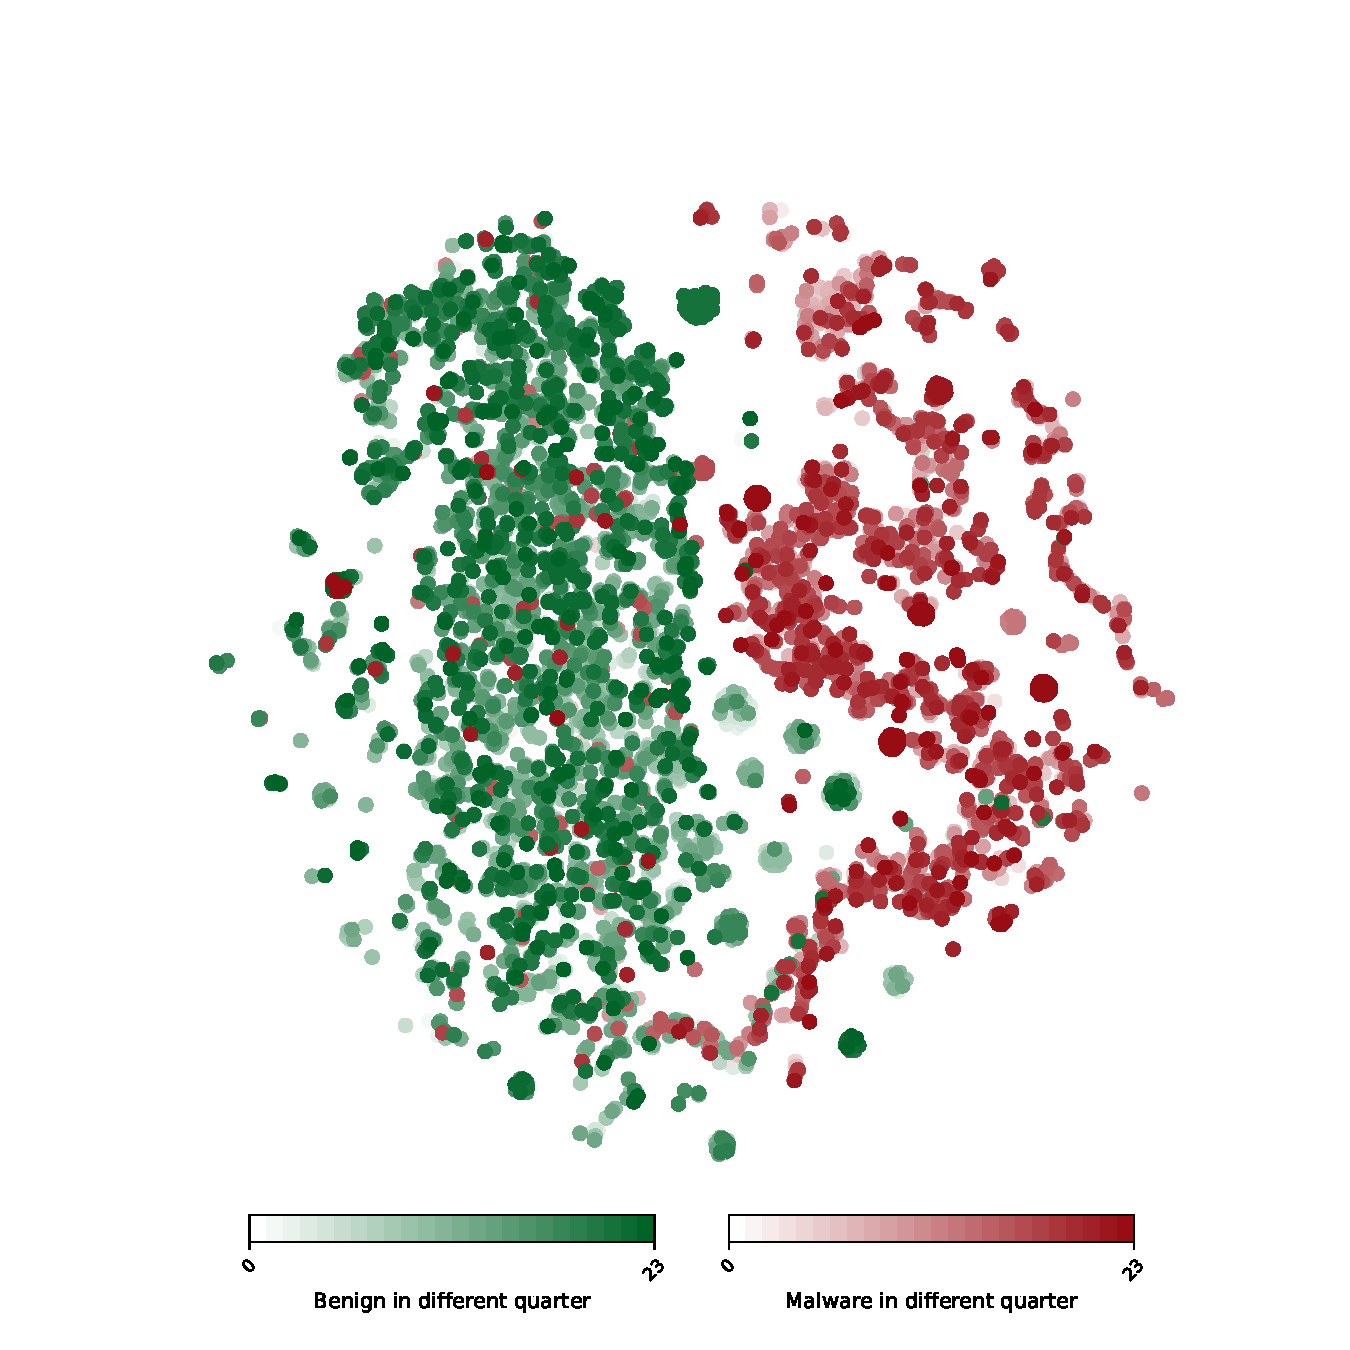
\includegraphics[width=3cm,height=3.5cm]{Graph/Motivation/tsne-APIGraph-v3}
%		\caption{APIGraph}
%		\label{fig::APIGraph PTXY concept drift dataset}
%	\end{subfigure}
%	\hspace{0.5cm}
%	\begin{subfigure}{0.20\textwidth}
%		\centering
%		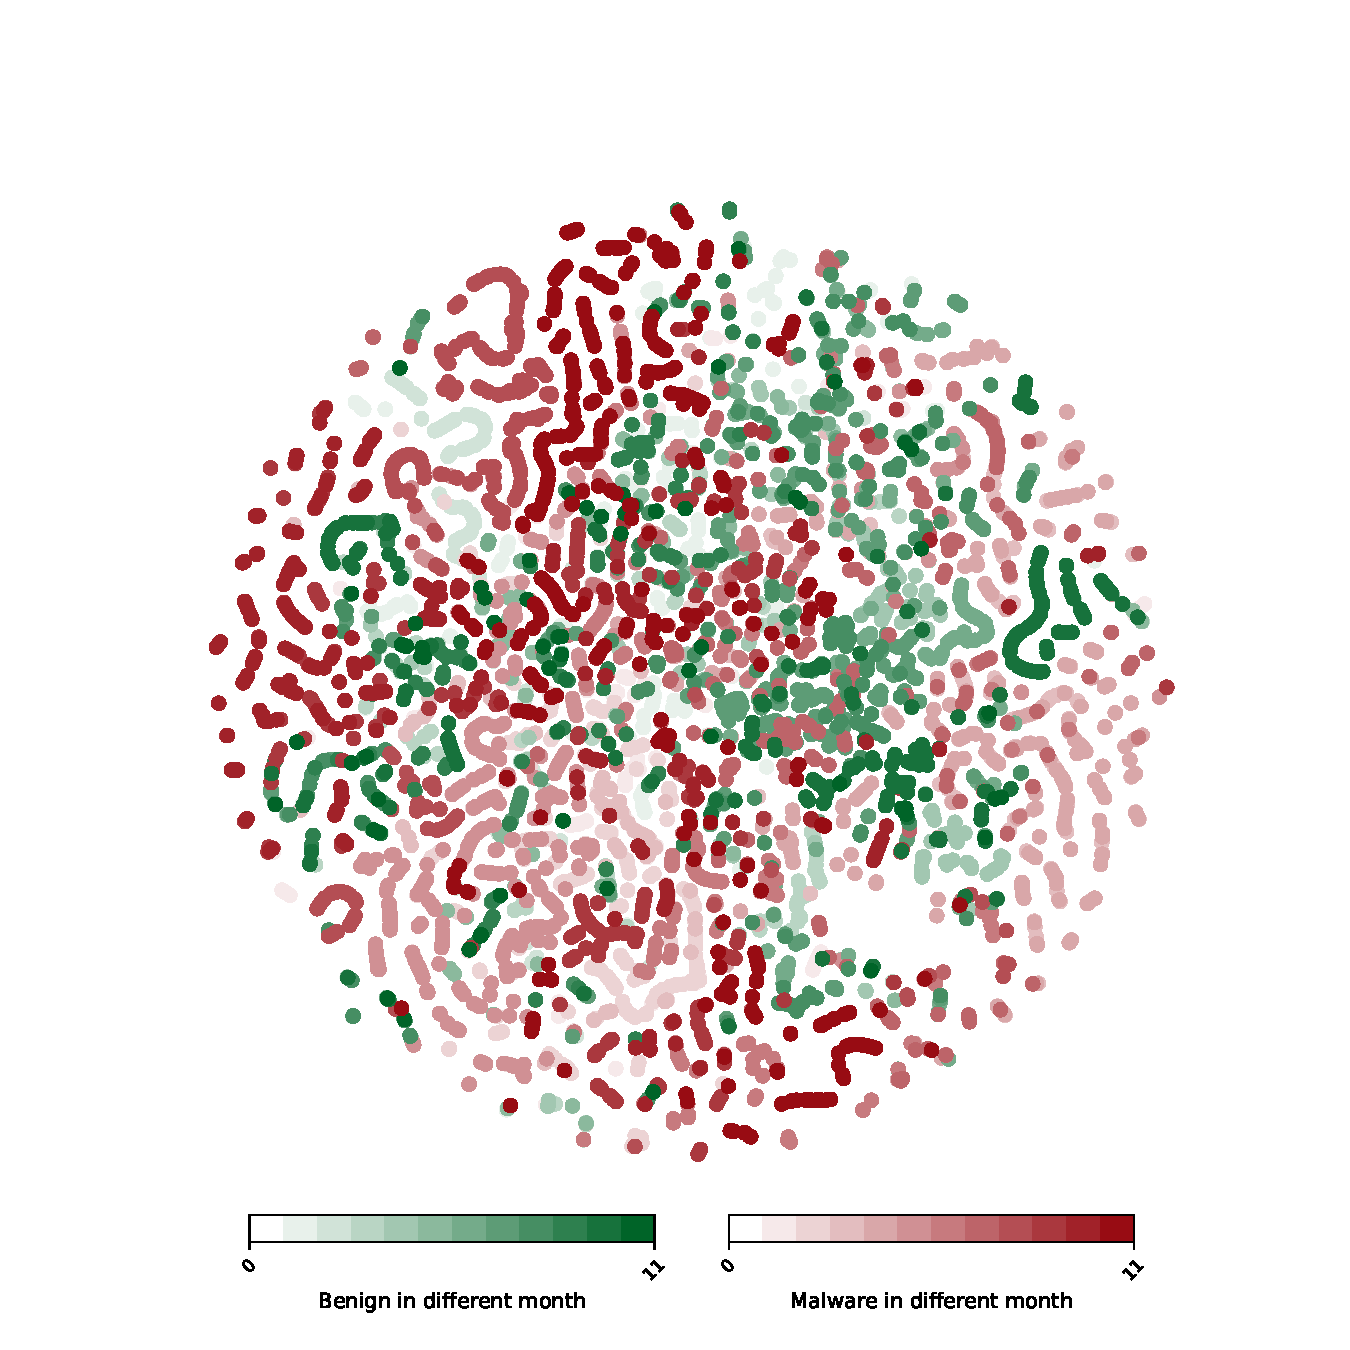
\includegraphics[width=3cm,height=3.5cm]{Graph/Motivation/tsne-BODMAS-v3}
%		\caption{BODMAS}
%		\label{fig::BODMAS PTXY concept drift dataset}
%	\end{subfigure}
%	\caption{T-SNE visualization of $P_{t}(\mathcal{X}|\mathcal{Y})$ concept drift in Android and Windows Malware Datasets}
%	\label{fig:PTXY concept drift in Malware Datasets}
%\end{figure}
%Malware samples may mimic benign characteristics or exhibit distinct malicious features, resulting in continuous changes in the feature distribution, as shown in Figure~\ref{fig:PTXY concept drift in Malware Datasets}.
%Consequently, at the time $t+1$, predicting the shift in $P_{t+1}(\mathcal{X}|\mathcal{Y})$ relative to $P_{t}\mathcal{X}|\mathcal{Y})$ becomes increasingly challenging.
%
%\noindent \textbf{(2) $P_{t}(\mathcal{Y})$ Concept Drift:} 
%Figure~\ref{fig:Attack Motivation-1} illustrates the quarterly distribution of the top 10 categories. 
%Given the significantly higher proportion of benign samples than malware samples, the largest category consists of benign samples, while the remaining nine are malicious families.
%Notably, the distribution shown reflects the label distribution of concept drift samples.
%\begin{figure}[htbp]
%	\centering
%	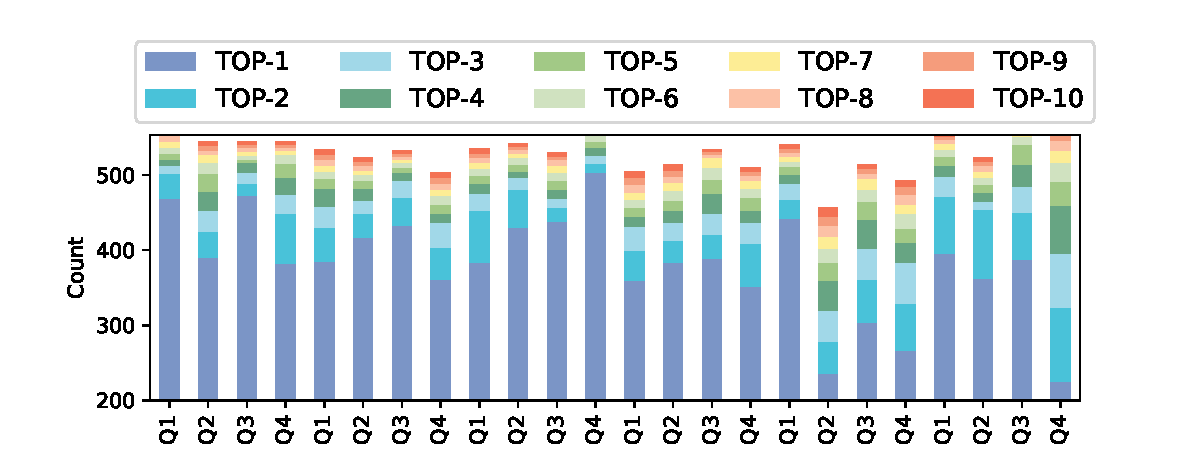
\includegraphics[width=\linewidth,keepaspectratio]{Graph/Evaluation/Figure2.pdf}
%	\caption{$P_{t}(\mathcal{Y})$ Concept Drift during 6 years}
%	\label{fig:Attack Motivation-1}
%\end{figure}
%In practice, the sample selection process is automated, leaving the model owner without access to any information about the distribution of concept drift samples before labeling.
%As a result, filtering poisoned samples becomes significantly more challenging.

\subsection{Shapley Additive Explanations}
\label{Sec: Shapley Additive Explanations}
Recent advances in explainable machine learning have introduced various methods for interpreting the predictions of complex models~\cite{ali2023explainable}.
SHapley Additive exPlanations~\cite{lundberg2017unified} adopt the Shapley value concept from cooperative game theory to assign each feature a contribution score based on its influence on the model's output.
The SHAP framework has been shown to subsume several earlier model explanation techniques~\cite{2021-Usenix-Poisoning-Attack-Explanation-guided-Backdoor}, including LIME~\cite{ribeiro2016should} and Integrated Gradients~\cite{sundararajan2017axiomatic}. 
These model explanation frameworks help determine the importance of each feature value in the model's prediction.
\begin{equation}
	\begin{aligned}
			g(\bm{\mathrm{x}}) = \phi_{0} + \sum_{j=1}^{M} \phi_{j} x_{j}
		\end{aligned}
	\label{SHAP}
\end{equation}
Explanation frameworks construct a surrogate linear model using the input feature vectors and output predictions, leveraging its coefficients to estimate feature importance and direction, as shown in Equation~\ref{SHAP}.
$\bm{\mathrm{x}}$ is the sample, $x_{j}$ is the $j^{th}$ feature for sample $\bm{\mathrm{x}}$, and $\phi_{j}$ is the contribution of feature $x_{j}$ to the model  prediction.
The SHAP framework stands out by providing theoretical guarantees for calculating feature contributions in a model-agnostic manner.
Recent studies have extended model prediction explanations to include explanations of prediction uncertainty~\cite{NEURIPS2023_16e4be78}.
Motivated by this, we incorporate SHAP-based uncertainty attribution into the design of our poisoning attack against concept drift adaptation methods.

\subsection{Concept Drift Dataset Settings}
\label{Sec: Concept Drift Dataset Settings}
Concept drift datasets have significantly advanced machine learning research due to their rich temporal attribute information.
However, collecting natural concept drift datasets poses challenges, as it incurs significant costs and demands accurate temporal attributes.
Therefore, synthetic datasets are often constructed for experimental evaluation in existing studies, in addition to real-world datasets.

\subsubsection{Synthetic Dataset Construction}
\label{Sec: Synthetic Concept Drift Dataset Construction}
In this experimental evaluation, we constructed synthetic concept drift datasets using a publicly available spam email dataset (SPAM-Email~\cite{2010-Spam-Emali-dataset}) and the MNIST image dataset~\cite{2017-MINIST-dataset}.

\begin{itemize}[leftmargin=*]
	\item[$\bullet$] \textbf{MNIST:} 
	We processed the MNIST handwritten digit dataset to simulate the concept drift phenomenon. 
	Specifically, we selected two clusters of digits, close in the feature space, to represent two classes: digits 3, 5, and 8 (labeled as 0) and digits 4, 7, and 9 (labeled as 1).
	Each digit is treated as a subclass, with new subclasses gradually introduced based on feature similarity to simulate gradual concept drift.
	We randomly selected 30\% of the data from digits 3 and 4 for the initial training set.
	The subsequent five cycles were used as testing periods, each selecting a portion of the unused data as the testing data.

	\item[$\bullet$] \textbf{SPAM-Email:} 
	Similar to the concept drift construction in the MNIST dataset, we conducted an in-depth analysis of the original SPAM dataset.
	Using sklearn's k-means algorithm with default parameters, we subdivided legitimate and spam emails into 12 clusters, each representing a distinct subclass.
	Based on this, we designed a concept drift partitioning scheme with nine cycles, each containing 1,036 samples and an approximate 3:1 ratio of legitimate to spam emails.
	To simulate concept drift, we introduced a new subclass of legitimate and spam emails in each cycle while ensuring data from the same subclass appeared in consecutive cycles to reflect emerging trends.
	The first cycle served as the training data, containing one subclass for legitimate emails and one for spam. In subsequent testing cycles, new subclasses were introduced, and the proportions of existing subclasses were adjusted, ensuring at least four subclasses were present in each cycle.
	This approach enabled a smooth evolution of the data distribution over time while ensuring orderly family replacement.
\end{itemize}

\subsection{Training and Testing Data Splits}
\label{Sec: Training and Testing Data Splits}
Most training and testing data partitions are static, with the model trained on the training dataset and evaluated on a fixed testing data.
However, testing data in concept drift scenarios are dynamic and continuously evolving.
Both the distribution and size of the testing data change as time progresses.

\begin{itemize}[leftmargin=*]
	\item[$\bullet$] \textbf{APIGraph:} The APIGraph\cite{2020-CCS-APIGraph} dataset is trained on data from 2012, with concept drift testing conducted on data from 2013 to 2018, where the data for each year is incrementally released monthly.
	The ratio of legitimate to malicious software for each year is roughly maintained at 9:1, simulating the real-world scenario where legitimate samples significantly outnumber malicious ones.
	Detailed data partitioning is provided in Table~\ref{tab: APIGraph Dataset}.

	\item[$\bullet$] \textbf{BODMAS:}
	The BODMAS~\cite{2021-PE-malware-dataset} dataset comprises 57,293 malware samples and 77,142 benign samples.
	The malware samples were randomly selected monthly from a security company's internal malware database, and data collection lasted from August 29, 2019, to September 30, 2020.
%	\begin{table}[t]
%		\begin{center}
%			\caption{Windows Malware Concept Drift Dataset} %鏍囬
%			\label{tab: BODMAS Dataset} %琛ㄦ爣绛?
%			\renewcommand{\arraystretch}{0.8}  % 璋冩暣璇ヨ〃鏍肩殑琛岃窛
%			\begin{tabular}{cccc} %c鐨勪釜鏁拌〃绀鸿〃鐨勫垪鏁?
%				\toprule
%				\textbf{Year} & \textbf{Malware} & \textbf{Benign} & \textbf{Malware Family}\\
%				\midrule
%				Train(before 10/19) & 4741 & 17655 & 330\\ 
%				Test-10/19 & 4549 & 3925 & 236 \\
%				Test-11/19 & 2494 & 3718 & 146 \\ 
%				Test-12/19 & 4039 & 6120 & 147 \\ 
%				Test-01/20 & 4510 & 5926 & 183 \\ 
%				Test-02/20 & 4269 & 3703 & 166 \\ 
%				Test-03/20 & 4990 & 3577 & 192 \\ 
%				Test-04/20 & 4640 & 5201 & 162 \\
%				Test-05/20 & 5449 & 6121 & 180 \\
%				Test-06/20 & 4217 & 8182 & 111 \\
%				Test-07/20 & 4995 & 6392 & 144 \\
%				Test-08/20 & 3823 & 2514 & 125 \\
%				Test-09/20 & 4577 & 4198 & 152\\
%				\midrule
%				\textbf{Total} & \textbf{57293} & \textbf{77142} & \textbf{2274} \\
%				\bottomrule
%			\end{tabular}
%		\end{center}
%	\end{table}

	\begin{table}[h!]
		\caption{Windows Malware Concept Drift Dataset}
		\label{tab: BODMAS Dataset}
		\setlength{\tabcolsep}{5.8pt}
		\begin{center}
			\scalebox{1.0}{
				\begin{tabular}{cccc}
					\toprule
					\textbf{Year}&\textbf{Malware}&\textbf{Benign} &\textbf{Malware Family} \\
					\midrule
					Train(before 10/19) & 4,741 & 17,655 & 330\\  
					Test-10/19 (Cycle 1) & 4,549 & 3,925 & 236 \\
					Test-11/19 (Cycle 2) & 2,494 & 3,718 & 146 \\
					Test-12/19 (Cycle 3) & 4,039 & 6,120 & 147 \\
					Test-01/20 (Cycle 4) & 4,510 & 5,926 & 183 \\ 
					Test-02/20 (Cycle 5) & 4,269 & 3,703 & 166 \\
					Test-03/20 (Cycle 6) & 4,990 & 3,577 & 192 \\ 
					Test-04/20 (Cycle 7) & 4,640 & 5,201 & 162 \\ 
					Test-05/20 (Cycle 8) & 5,449 & 6,121 & 180 \\ 
					Test-06/20 (Cycle 9) & 4,217 & 8,182 & 111 \\ 
					Test-07/20 (Cycle 10) & 4,995 & 6,392 & 144 \\ 
					Test-08/20 (Cycle 11) & 3,823 & 2,514 & 125 \\
					Test-09/20 (Cycle 12) & 4,577 & 4,198 & 152 \\
					\specialrule{0.05em}{1pt}{1pt}
					\textbf{Total} & \textbf{57,293} & \textbf{77,142} & \textbf{2,274} \\
					\bottomrule
			\end{tabular}}
		\end{center}
	\end{table}

	The data collected before October 2019 is used as the initial training data, while the data collected afterward serves as the concept drift testing data, as shown in Table~\ref{tab: BODMAS Dataset}.
	The testing data is evaluated every month.

	\item[$\bullet$] \textbf{SPAM-Email:}
	The dataset contains spam and legitimate messages, with a moderate spam ratio of approximately 25\%.
	It includes 9,324 instances and 500 features.
	The initial training data consists of 771 legitimate emails and 265 spam emails.
	Subsequently, 265 new spam emails and 771 legitimate emails are introduced in each of the 8 concept drift testing cycles.
%	\begin{table}[htbp]
%		\begin{center}
%			\caption{Synthetic Concept Drift Dataset for SPAM-Email} %鏍囬
%			\label{tab: Synthetic Concept Drift Dataset for SPAM-Email} %琛ㄦ爣绛?
%			\renewcommand{\arraystretch}{0.8}  % 璋冩暣璇ヨ〃鏍肩殑琛岃窛
%			\begin{tabular}{ccc} %c鐨勪釜鏁拌〃绀鸿〃鐨勫垪鏁?
%				\toprule
%				\textbf{miner} & \textbf{Spam} & \textbf{Legitimate} \\
%				\midrule
%				Train & 265 & 771 \\ 
%				Test-1 & 265 & 771 \\ 
%				Test-2 & 265 & 771 \\ 
%				Test-3 & 265 & 771 \\ 
%				Test-4 & 265 & 771 \\ 
%				Test-5 & 265 & 771 \\ 
%				Test-6 & 265 & 771 \\
%				Test-7 & 265 & 771 \\
%				Test-8 & 265 & 771 \\
%				\midrule
%				\textbf{Total} & \textbf{2387} & \textbf{6937} \\
%				\bottomrule
%			\end{tabular}
%		\end{center}
%	\end{table}

		\begin{table}[h!]
		\caption{Synthetic Concept Drift Dataset for SPAM-Email}
		\label{tab: Synthetic Concept Drift Dataset for SPAM-Email}
		\setlength{\tabcolsep}{5.8pt}
		\begin{center}
			\scalebox{1.0}{
				\begin{tabular}{ccc}
					\toprule
					\textbf{miner} & \textbf{Spam} & \textbf{Legitimate} \\
					\midrule
					Train & 265 & 771 \\ 
					Test-1 (Cycle 1) & 265 & 771 \\ 
					Test-2 (Cycle 2) & 265 & 771 \\ 
					Test-3 (Cycle 3) & 265 & 771 \\ 
					Test-4 (Cycle 4) & 265 & 771 \\ 
					Test-5 (Cycle 5) & 265 & 771 \\ 
					Test-6 (Cycle 6) & 265 & 771 \\
					Test-7 (Cycle 7) & 265 & 771 \\
					Test-8 (Cycle 8) & 265 & 771 \\
					\specialrule{0.05em}{1pt}{1pt}
					\textbf{Total} & \textbf{2,387} & \textbf{6,937} \\
					\bottomrule
			\end{tabular}}
		\end{center}
	\end{table}

	\item[$\bullet$] \textbf{MNIST:}
	The MNIST dataset contains handwritten digits. 
	3,591 samples were used for training, and 31,860 samples were distributed across 5 concept drift testing cycles.
%	\begin{table}[htbp]
%		\begin{center}
%			\caption{Synthetic Concept Drift Dataset for MNIST} %鏍囬
%			\label{tab: Synthetic Concept Drift Dataset for MNIST} %琛ㄦ爣绛?
%			\renewcommand{\arraystretch}{0.8}  % 璋冩暣璇ヨ〃鏍肩殑琛岃窛
%			\begin{tabular}{ccc} %c鐨勪釜鏁拌〃绀鸿〃鐨勫垪鏁?
%				\toprule
%				\textbf{Year} & \textbf{Label-1} & \textbf{Label-0} \\
%				\midrule
%				Train & 1752 & 1839 \\ 
%				Test-1 & 1752 & 2923 \\ 
%				Test-2 & 2421 & 2852 \\ 
%				Test-3 & 2463 & 2867 \\ 
%				Test-4 & 2734 & 2603 \\ 
%				Test-5 & 6930 & 4315 \\ 
%				\midrule
%				\textbf{Total} & \textbf{18052} & \textbf{17399} \\
%				\bottomrule
%			\end{tabular}
%		\end{center}
%	\end{table}

	\begin{table}[h!]
	\caption{Synthetic Concept Drift Dataset for MNIST}
	\label{tab: Synthetic Concept Drift Dataset for MNIST}
	\setlength{\tabcolsep}{5.8pt}
	\begin{center}
		\scalebox{1.0}{
			\begin{tabular}{ccc}
				\toprule
				\textbf{Year} & \textbf{Label-1} & \textbf{Label-0} \\
				\midrule
				Train & 1,752 & 1,839 \\ 
				Test-1 (Cycle 1) & 1,752 & 2,923 \\ 
				Test-2 (Cycle 2) & 2,421 & 2,852 \\ 
				Test-3 (Cycle 3) & 2,463 & 2,867 \\ 
				Test-4 (Cycle 4) & 2,734 & 2,603 \\ 
				Test-5 (Cycle 5) & 6,930 & 4,315 \\
				\specialrule{0.05em}{1pt}{1pt}
				\textbf{Total} & \textbf{18,052} & \textbf{17,399} \\
				\bottomrule
		\end{tabular}}
	\end{center}
\end{table}

\end{itemize}


%\subsection{Victim Model Settings}
%\label{Sec: Victim Model Settings}
%We adopt commonly used or well-performing architectures from prior research~\cite{2023-Usenix-chenyizhen,2022-SP-Trancending,2021-Usenix-CDAE} in machine learning tasks for the victim model setup. 
%All experiments are conducted on a Windows 11 system with 96GB memory, one Intel庐 Core鈩?i7-14700K 3.4GHz CPU, and an NVIDIA GeForce RTX 4080 SUPER (16GB).
%We present the model parameters optimized for respective classification tasks.
%\begin{table}[htbp]
%	\centering
%	\small
%	\caption{Parameters Setting of CDA-AL}
%	\label{tab: Parameter setting of active learning method}
%	%\renewcommand{\arraystretch}{1.2} % 璋冩暣鍗曞厓鏍奸珮搴?
%	\begin{tabular}{c|c c}
%		\hline
%		\textbf{Parameter} & \textbf{APIGraph} & \textbf{MNIST}\\ \hline
%		Optimizer  & SGD & ADAM\\ 
%		LR & 0.003 & 0.0004\\ 
%		Batch size & 1024 & 64\\ 
%		Loss & hi-dist-xent & triplet-mse\\ 
%		LR decay & 0.05 & - \\ 
%		Decay epochs & 10,500,10 & -\\
%		Learning epochs & 50 & 5\\ 
%		\hline
%		\textbf{Parameter} & \textbf{BODMAS} & \textbf{SPAM-Email} \\
%		\hline
%		Optimizer & AdamW & AdamW \\ 
%		LR & 0.0004 & 0.0004 \\ 
%		Batch size & 64 & 64 \\ 
%		Loss & BCE & BCE \\ 
%		LR decay & - & - \\ 
%		Decay epochs & - & - \\
%		Learning epochs & 50 & 5\\ 
%	\end{tabular}
%\end{table}
%Table~\ref{tab: Parameter setting of active learning method} summarizes the parameter settings for experiments conducted on four datasets: APIGraph~\cite{2020-CCS-APIGraph}, MNIST~\cite{2017-MINIST-dataset}, BODMAS~\cite{2021-PE-malware-dataset}, and SPAM-Email~\cite{2010-Spam-Emali-dataset}.
%APIGraph: SGD optimizer with a learning rate (LR) of 0.003, batch size 1024, and hi-dist-xent loss function.
%The learning rate decay was set to 0.05 and applied at epochs 10, 500, and 10.
%The model was trained for 50 epochs.
%MNIST: Adam optimizer with an LR of 0.0004, batch size 64, and triplet-my loss function. 
%No learning rate decay was applied, and the model was trained for five epochs.
%BODMAS and SPAM-Email: AdamW optimizer with an LR of 0.0004, batch size 64, and binary cross-entropy (BCE) loss function.
%No learning rate decay was applied.
%The model was trained for 50 epochs on BODMAS and five epochs on SPAM-Email.

	
\begin{figure*}[ht]
	%\setlength{\belowcaptionskip}{-1.5em} % 鎺у埗鍥剧墖鏍囬涓庡悗缁枃鏈箣闂寸殑闂磋窛
	\centering
	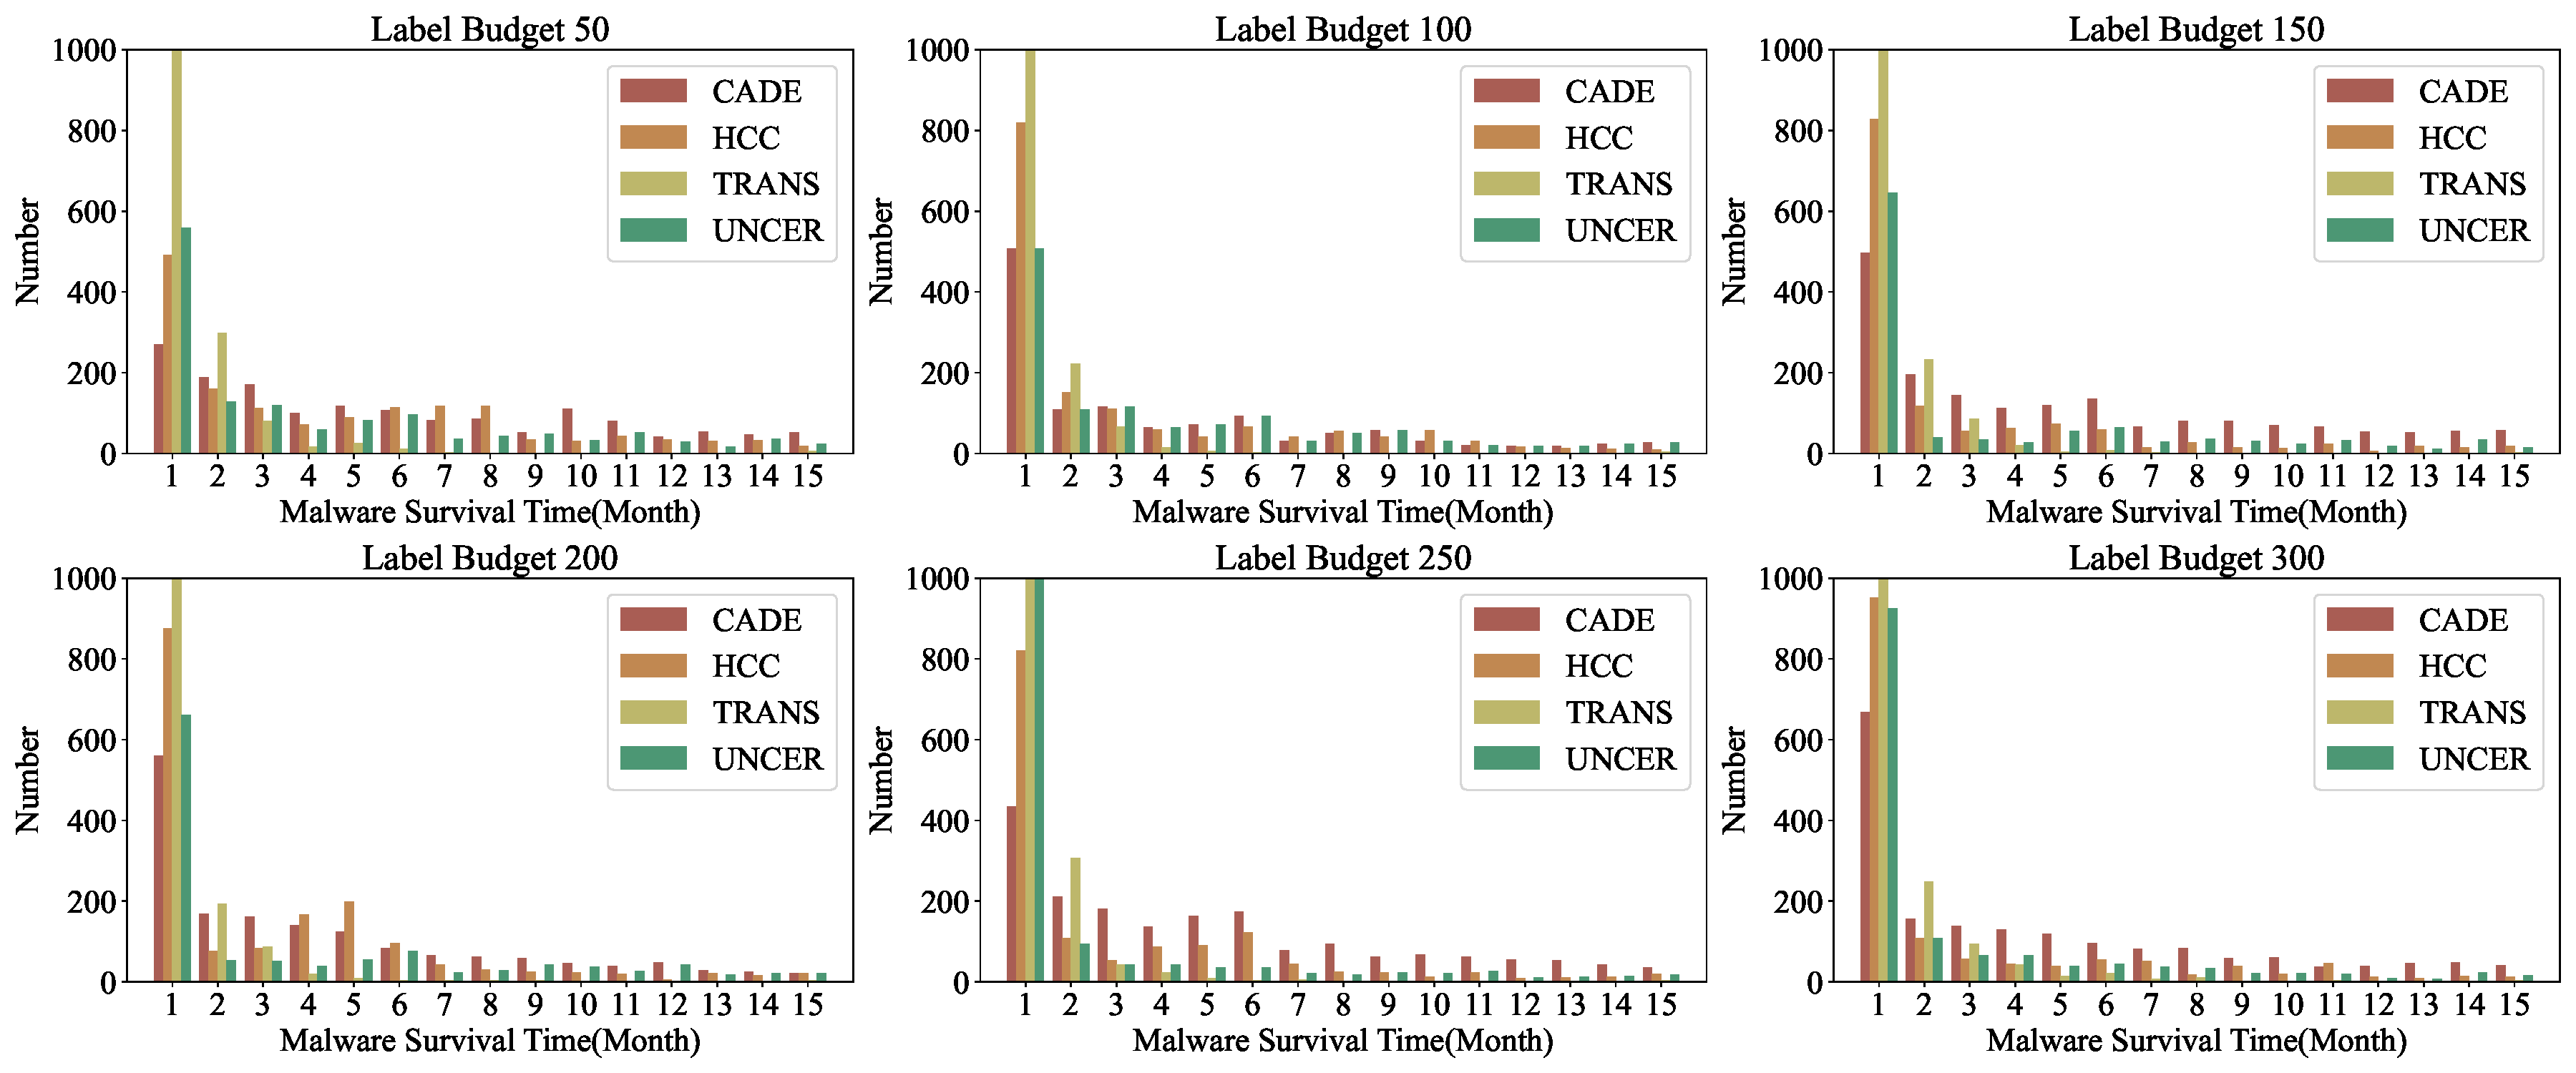
\includegraphics[width=\linewidth,keepaspectratio]{Graph/Appendix/Original_threat_life_cycle_all_budget_0901.pdf}
	\caption{Original misclassification time of attack targets}
	\label{fig: Original survival time of all budget}
\end{figure*}
%\subsection{Concept Drift Adaptation Strategies}
%\label{Sec: Concept Drift Adaptation Strategies}
%
%
%%\textbf{Model Uncertainty.} The core idea of uncertainty measurement~\cite{2023-survey-uncertainty-in-deep-neural-networks} is to detect concept drift based on the output layer of the target model. 
%%The model gives priority to selecting the samples with high uncertainty of the current model for labeling. 
%%A common uncertainty measurement for a neural network is to use one minus the max softmax output of the network.
%
%\noindent \textbf{ (1) Encoder Space Distance (CADE):} CADE~\cite{2021-Usenix-CDAE} trains an encoder through existing labeled data for learning a compressed representation (dimension reduction) of a given input distribution. 
%Then, the newly obtained test samples can be provided to the encoder to obtain the encoder's spatial features. 
%Finally, the distance function can effectively identify concept drift samples far from the existing training dataset.
%
%\noindent \textbf{(2) Credibility and Confidence (TRANS):} Transcending~\cite{2022-SP-Trancending} introduced the thery of conformal prediction~\cite{2005-high-cite-Algorithmic-learning-in-a-random-world} (credibility and confidence) into the field of concept drift adaptation. 
%Given a new test sample, Transcending first computes the non-conformity score of the sample. 
%Then, it computes credibility as the percentage of samples in the calibration set that have higher non-conformity scores than the test sample. 
%Finally, it computes confidence as one minus the credibility of the opposite label. 
%A lower credibility score or a lower confidence score means the test sample is more likely to have drifted.

%\noindent \textbf{(3) Hierarchical Contrastive Loss (HCL):} The method proposed by Chen et al.~\cite{2023-Usenix-chenyizhen} is currently the best-performing strategy in Android malware concept drift adaptation methods. 
%The model consists of two modules. 
%The first module is an encoder and the second module acts as the classifier. 
%In terms of loss function settings, to ensure that the model is robust to concept drift, the training loss of the model is set to the sum of hierarchical contrast loss and classification loss.
%The advantage of this strategy is its provision of finer-grained encoder rules and utilization of similar features among malware families, ultimately enhancing concept drift adaptation performance.


% 2025-Usenix-鎶曠鎷掔粷
%\section{Original Survival Time of All Label Budget}
%\label{Sec: Original Survival Time of All Label Budget}
%
%\noindent We have analyzed the survival time of new malware under different label budget settings and various concept drift adaptation strategies, as shown in Figure \ref{fig: Original survival time of all budget}. 
%We can observe that the survival time of new malware exhibits a consistent trend, regardless of the label settings and concept drift adaptation strategies.
%Most new malware can survive for 1-5 months under concept drift adaptation strategies, a small portion can survive for more than 5 months, while the survival time of most old malware samples is 0.
%Moreover, most concept drift adaptation strategies face the situation that some new malware survives for more than one year under sufficient label budget (300 samples).
%This phenomenon fully indicates that there is still room for improvement in the performance of the current concept drift adaptation strategies.
%Due to the uneven distribution of survival times for new malware samples under the TRANS concept drift adaptation strategy, the number of samples with survival times of 0-2 months exceeds five times that of samples in other time intervals. 
%Therefore, for the sake of convenient presentation, we have truncated the bar chart representing the 0-2 months survival time samples in the TRANS statistics, while preserving the relative proportions of the overall sample volumes.
%\begin{figure*}[ht!]
%	%\setlength{\belowcaptionskip}{-1em} % 鎺у埗鍥剧墖鏍囬涓庡悗缁枃鏈箣闂寸殑闂磋窛
%	\centering
%	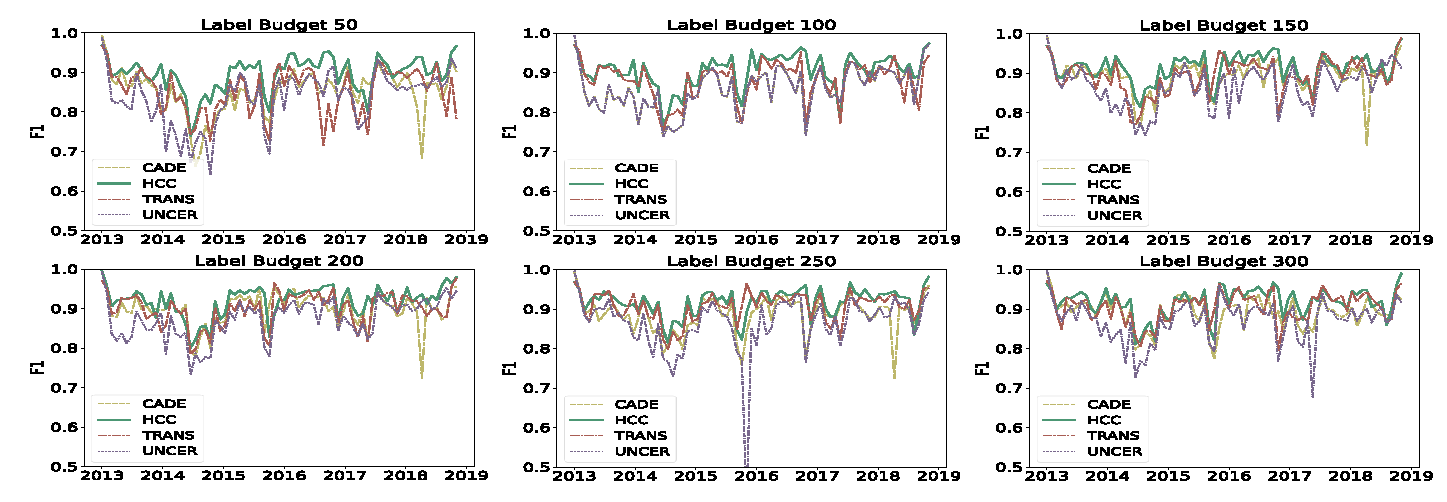
\includegraphics[width=\linewidth,keepaspectratio]{Graph/Appendix/base_performance_allbudget_0830.pdf}
%	\caption{Concept drift adaptation baseline}
%	\label{fig: CDA-AL Baseline}
%\end{figure*}

% \label{sec: Testing of attack overhead in problem space}
% %\vspace{-1em}
% \begin{table}[H]
	% \centering
	% \caption{APK obfuscation time}
	% %\renewcommand{\arraystretch}{0.8}  % 璋冩暣璇ヨ〃鏍肩殑琛岃窛
	% \label{tab: APK obfuscation time}
	% \begin{tabular}{c|c|c|c}
		% \toprule
		% \textbf{APK} & \textbf{Size(MB)} & \textbf{Category} & \textbf{Obfuscation} \\
		% \midrule
		% \textbf{JD} & 97.59 & shopping & 54.95s \\
		% \textbf{Taobao} & 57.03 & shopping & 78.98s \\
		% \textbf{Little Red Book} & 162.99 & social & 178.68s \\
		% \textbf{Google} & 315.67 & tool & 93.32s \\
		% \textbf{Wang VPN} & 45.51 & tool & 14.91s \\
		% \textbf{WeChat} & 264.04 & communication & 136.76s \\
		% \midrule
		% \textbf{Average} & 199.72 & - & 90.72s \\
		% \bottomrule
		% \end{tabular}
	% \end{table}

% 杩欎釜鍏堜笉璇翠簡
% \textbf{Feature Space Inverse Mapping:} In the end, we need to show that the features corresponding to the poison samples must have corresponding Android applications in the problem space. Since an attack seed sample is an object in the problem space that meets semantic requirements, and the poison samples are single-bit flip variants of the attack seed sample in the feature space, so they also meet semantic requirements in the problem space. For feature spaces such as the APIGraph dataset and the Androzoo dataset, a single transformation means an increase or decrease in an API call or permission declaration. 

%\section{Concept Drift Adaptation Strategy Settings}
%\label{sec: Concept Drift Adaptation Strategy Settings}
%\noindent It is not enough to just enumerate the model structures and concept drift adaptation strategies. 
%What is more critical is to combine them. 
%Our combination follows the principle of optimal configuration. 
%For each target model structure, we select the corresponding concept drift adaptation strategy based on the optimal combination method in existing research methods.
%The last setting about the concept drift adaptation strategy is the initial state of the target model. 
%Our setting in this study is to train the initial data for 1 year, then conduct PACDA attack verification, and use the monthly time window to evaluate and verify the effectiveness of the attack.
%The final combination is shown in Table \ref{tab: Combination of Model Structure and CDA-Strategy}.

%\section{Concept Drift Adaptation Baseline}
%\label{sec: CDA-AL Baseline}
%\noindent We conduct baseline tests on the performance of current mainstream concept drift adaptation methods on the APIGraph~\cite{2020-CCS-APIGraph} and CDAMAL\footnote{\url{https://anonymous.4open.science/r/Denial-of-Concept-Drift-Adaptation-Contribution-343C}} datasets, and the test results are shown in the Figure \ref{fig: CDA-AL Baseline}. 
%We run all experiments on a Win11 with 96GB memory, 1 Intel (R) Core (TM)i7-14700K 3.4GHz CPU and one NVIDIA GeForce RTX 4080 SUPER (16GB). 
%\begin{comment}
%	\begin{table}[h]
%		\centering
%		\small
%		\caption{Parameter setting of active learning method}
%		\label{tab: Parameter setting of active learning method}
%		%\renewcommand{\arraystretch}{1.2} % 璋冩暣鍗曞厓鏍奸珮搴?
%		\begin{tabular}{c|c c}
%			% \hline
%			\multirow{2}{*}{Parameter} & \multicolumn{2}{c}{Method} \\ \cline{2-3} 
%			& \textbf{HCL} & \textbf{CADE}\\ \hline
%			Optimizer  & SGD & ADAM\\ 
%			LR & 0.003 & 0.0001\\ 
%			Batch size & 1024 & 32\\ 
%			Loss & hi-dist-xent & triplet-mse\\ 
%			LR decay & 0.05 & 1\\ 
%			Decay epochs & 10,500,10 & 10,500,10\\
%			Scheduler & step & cosine\\ 
%			Learning epochs & 50 & 50\\ 
%			\hline
%			Parameter & \textbf{TRANS} & \textbf{UNC} \\
%			\hline
%			Optimizer & SGD & SGD \\ 
%			LR & 0.003 & 0.003 \\ 
%			Batch size & 512 & 1024 \\ 
%			Loss & hi-dist & hi-dist-xent \\ 
%			LR decay & 0.95 & 0.95 \\ 
%			Decay epochs & 10,500,10 & 30,1000,30 \\
%			Scheduler & step & step \\ 
%			Learning epochs & 50 & 50\\ 
%		\end{tabular}
%	\end{table}
%\end{comment}
%Here, we offer a concise overview of the hyperparameter configurations. 
%We utilize the SGD optimizer for HCL, TRANS, and UNC while employing the ADAM optimizer for CADE. 
%For the loss functions, TRANS uses the Hierarchical Distance loss function, CADE uses the Triplet Mean Squared Error loss function, and HCL and UNC employe the Hierarchical Distance Cross-Entropy loss function. 
%The total number of training epochs is set to 50 for all four methods.
%More detailed hyperparameter settings are shown in Table \ref{tab: Parameter setting of active learning method}.
%In this study, we test four types of current mainstream excellent Android malware detection models~\cite{2020-CCS-APIGraph,2023-TIFS-Federated-Android-Malware-ResNet,2023-Usenix-chenyizhen}, and the obtained concept drift detection data is shown in Figure \ref{fig: CDA-AL Baseline}.
%It can be observed that the higher the label budget setting is, the better the performance of the concept drift adaptation method becomes.
%Moreover, the latest concept drift adaptation method (HCL~\cite{2023-Usenix-chenyizhen}) demonstrates performance advantage over the existing methods (TRANS~\cite{2022-SP-Trancending},CADE~\cite{2021-Usenix-CDAE},UNCER~\cite{2023-survey-uncertainty-in-deep-neural-networks}).
%We notice that the performance of existing concept drift adaptation strategies is unstable, and even the optimal HCL method has performance fluctuations.
%The instability also inspires the research on the security of concept drift adaptation strategies in our study.

%As can be seen from the figure, after 6 years, the detector's F1 score index averaged 0.73 per month, a decrease of 0.26 compared to the initial month, and the lowest point dropped to 0.32 in November 2015, with an FNR as high as 77.66\%.

% \begin{table}[h]
	% \centering
	% \small
	% \caption{Parameter setting of active learning method}
	% \label{tab: Parameter setting of active learning method}
	% %\renewcommand{\arraystretch}{1.2} % 璋冩暣鍗曞厓鏍奸珮搴?
	% \begin{tabular}{c|c c c c }
		% % \hline
		% \multirow{2}{*}{\textbf{Parameter}} & \multicolumn{4}{c}{\textbf{Method}} \\ \cline{2-5} 
		%  & \textbf{HCC} & \textbf{CADE} & \textbf{TRANS} & \textbf{UNC} \\ \hline
		% \textbf{Optimizer}  & SGD & ADAM & SGD & SGD \\ 
		% \textbf{LR} & 0.003 & 0.0001 & 0.003 & 0.003 \\ 
		% \textbf{Batch size} & 1024 & 32 & 512 & 1024 \\ 
		% \textbf{Loss} & hi-dist-xent & triplet-mse & hi-dist & hi-dist-xent \\ 
		% \textbf{LR decay} & 0.05 & 1 & 0.95 & 0.95 \\ 
		% \textbf{Decay epochs} & 10,500,10 & 10,500,10 & 10,500,10 & 30,1000,30 \\
		% \textbf{Scheduler} & step & cosine & step & step \\ 
		% \textbf{learning epochs} & 50 & 50 & 50 & 50 \\ 
		% \end{tabular}
	% \end{table}



%\section{Freeze Attack Strategy}
%\label{Sec: Attack Value Unstable}
%%\begin{figure}[h]
%%	%\setlength{\belowcaptionskip}{-1em} % 鎺у埗鍥剧墖鏍囬涓庡悗缁枃鏈箣闂寸殑闂磋窛
%%	\centering    
%%	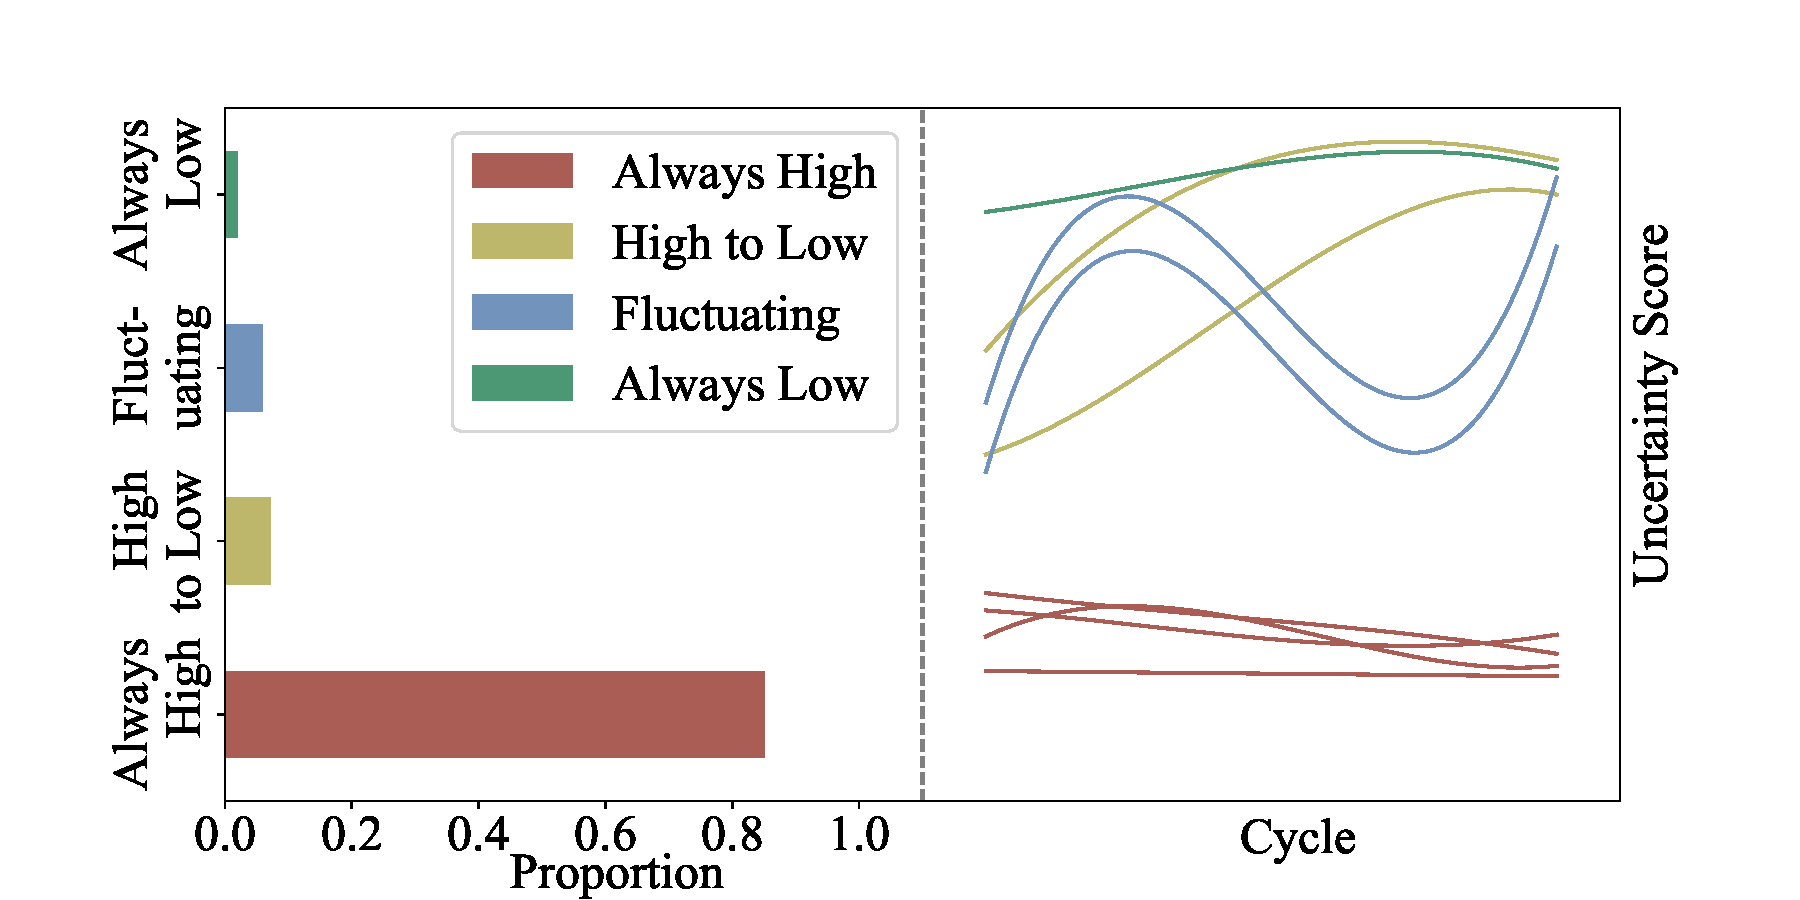
\includegraphics[width=\linewidth,keepaspectratio]{Graph/Appendix/attack_value_change_0830.pdf}       	
%%	\caption{Attack value unstable}
%%	\label{fig: Attack Value Unstable}
%%\end{figure}
%%%It is important to note that the PACDA attack framework is an automated attack framework, which needs to continuously generate poisoned samples in each model cycle.
%%Therefore, the malware attack value assessment module and the survival time prolongation module need to be integrated with each model cycle. 
%
%\noindent We observe that the attack value of new high uncertainty malware in the initial model cycle also exhibits instability in subsequent model cycles.
%%, as shown in Figure \ref{fig: Attack Value Unstable}. 
%While 85\% of the samples maintain a high attack value in the subsequent cycles, nearly 15\% of the samples experience fluctuations in their attack value.
%Specifically, the attack value of the samples may oscillate between high and low values, or it may shift from high value to low value. 
%To ensure the consistency of attack effectiveness across consecutive model cycles, we employ freeze attacks during the low attack value model cycles of new malware. 
%Freeze attack involves selecting benign poisoned seed samples with the highest uncertainty score. 
%During the poisoned sample generation phase, data augmentation based on sample replication strategies is applied to produce a batch of attack samples.


% 鐩稿叧宸ヤ綔鐨勮繖閮ㄥ垎涓嶆斁姝f枃浜嗭紝淇℃伅閲忓お灏戯紝閮芥槸鍓嶉潰璇磋繃鐨勪笢瑗?
% \textbf{Concept Drift Adaptation.} Currently, researchers believe that the phenomenon of concept drift is the main reason affecting the survival time of new malware. Researchers have proposed a series of methods~\cite{2023-Usenix-chenyizhen,2022-SP-Trancending,2021-Usenix-CDAE,2017-Usenix-Transcend} to detect concept drift samples and optimize models. Furthermore, Yiling He et al.~\cite{2024-arxiv-Going-Proactive-and-Explanatory-Against-Malware-Concept-Drift} have proposed DREAM, a method that can effectively enhance the accuracy of drift detection and reduce the cost of manual analysis. Our work primarily focuses on detecting concept drift, as this phase serves as the foundation for subsequent stages. While existing research has mainly concentrated on optimizing the performance of adaptation methods for concept drift, our emphasis lies on its security.

\subsection{Attack Target List}
\label{Sec: Attack Target List}
The experimental evaluation was conducted under various attack target configurations to validate the effectiveness of the proposed method and to analyze factors influencing attack success.
The detailed information is as follows.

\begin{itemize}[leftmargin=*]

	\item[$\bullet$] \textbf{Single-Target Attack:} 
	We followed two principles when selecting attack targets.
	First, the attack target must not be included in the training set.
	Second, the attack target is misclassified during the month it appears.
	This indicates that the attack target is a newly emerging concept drift sample in the testing phase rather than a simple modification of existing samples in the training data.
	Moreover, this also prevents situations where the attack target lacks sufficient attack value.

	\item[$\bullet$] \textbf{Multi-Target Attack:} 
	The attack targets for multi-target attacks are composed of multiple single-attack targets that emerge simultaneously.
	The targets of APIGraph are detailed in Table~\ref{tab: Attack Target for Multi-target Attack}.
	The concept drift adaptation associated with the attack target spans five years.
	For other datasets, the multi-target attack is conducted over the entire set of attack targets.
	\begin{table}[ht!]
		\begin{center}
			\caption{Attack Target for Multi-target Attack} %鏍囬
			\label{tab: Attack Target for Multi-target Attack} %琛ㄦ爣绛?
			\renewcommand{\arraystretch}{0.8}  % 璋冩暣璇ヨ〃鏍肩殑琛岃窛
			\begin{tabular}{ccc} %c鐨勪釜鏁拌〃绀鸿〃鐨勫垪鏁?
				\toprule
				\textbf{Month} & \textbf{Type} & \textbf{Family} \\
				\midrule
				\multirow{6}{*}{2013-09} & \multirow{3}{*}{Non-Target} 	& ansca \\ 
				&	& cardserv \\ 
				&	& svpeng  \\ \cline{2-3}
				& \multirow{3}{*}{Target} 	& mecor  \\
				&	& smforw \\
				&	& vietsms \\
				\midrule
				\multirow{5}{*}{2014-05} & \multirow{3}{*}{Non-Target} 	& gabas \\ 
				&	& simplocker \\ 
				&	& smssend \\ \cline{2-3}
				& \multirow{2}{*}{Target} 	& mecor  \\
				&	& svpeng  \\ 
				\midrule
				\multirow{6}{*}{2014-06} & \multirow{4}{*}{Non-Target} 	& chyapo \\ 
				&	& pletor \\
				&	& spyware \\
				&   & tebak   \\ \cline{2-3}
				& \multirow{2}{*}{Target} 	& mecor \\
				&   & adflex  \\
				\midrule
				\multirow{5}{*}{2014-09} & \multirow{3}{*}{Non-Target} 	& fobus \\ 
				&	& gamecheater \\
				&   & ransomware  \\ \cline{2-3}
				& \multirow{2}{*}{Target} 	& mecor \\
				&   & spyware  \\
				\midrule
				\multirow{5}{*}{2014-10} & \multirow{3}{*}{Non-Target} 	& fakebank \\ 
				&	& systemmonitor \\
				&   & webapp  \\ \cline{2-3}
				& \multirow{2}{*}{Target} 	& airpush \\
				&   & mecor  \\
				\midrule
				\multirow{5}{*}{2015-05} & \multirow{3}{*}{Non-Target} 	& adflex \\ 
				&	& kalfere \\
				&   & styricka  \\ \cline{2-3}
				& \multirow{2}{*}{Target} 	& mobidash \\
				&   & vnapstore  \\
				\midrule
				\multirow{4}{*}{2016-07} & \multirow{1}{*}{Non-Target} 	& clicks \\  \cline{2-3}
				& \multirow{3}{*}{Target} 	& adflex \\
				&   & blouns  \\
				&   & mspy    \\
				\midrule
				\multirow{3}{*}{2017-01} & \multirow{1}{*}{Non-Target} 	& mobidash \\  \cline{2-3}
				& \multirow{2}{*}{Target} 	& batmob \\
				&   & kalfere  \\
				\midrule
			\end{tabular}
		\end{center}
	\end{table}

	%\noindent \textbf{(3) Dynamic Switching Between Different Attack Target Configurations:} 
	%The target selection rules are the same as those for the multi-target attack scenario.
	%The attack targets are detailed in Table~\ref{tab: Attack Target for Dynamic Switching}.
	%\begin{table}[htbp]
	%	\begin{center}
		%		\caption{Attack Target for Dynamic Switching} %鏍囬
		%		\label{tab: Attack Target for Dynamic Switching} %琛ㄦ爣绛?
		%		\renewcommand{\arraystretch}{0.8}  % 璋冩暣璇ヨ〃鏍肩殑琛岃窛
		%		\begin{tabular}{cc|cc} %c鐨勪釜鏁拌〃绀鸿〃鐨勫垪鏁?
			%			\toprule
			%			\textbf{Month} & \textbf{Family} & \textbf{Month} & \textbf{Family} \\
			%			\midrule
			%			\multirow{5}{*}{2014-09} & mecor & \multirow{5}{*}{2015-01} & airpush\\ 
			%									 & spyware &  & mobidash \\ 
			%									 & gamecheater &  & svpeng \\ 
			%									 & ransomware &  & kemoge \\ 
			%									 & fobus &  & gorpo \\ 
			%			\midrule
			%			\multirow{4}{*}{2016-07} & clicks & \multirow{4}{*}{2018-01} & itracker\\ 
			%									& adflex &  & faketoken \\ 
			%									& blouns &  & clicks \\ 
			%									& mspy &  & miner \\ 
			%			\midrule
			%		\end{tabular}
		%	\end{center}
	%\end{table}
\end{itemize}



\subsection{Attack Target Initial Misclassification Time}
\label{Sec: Attack Target Initial Survival Time (APIGraph)}
Since the effectiveness of the PACDA is defined by prolonging the misclassification duration of the original attack target, it is essential to test the misclassification duration of the attack target in the absence of any attacks.
We analyzed the misclassification time of malware under different labeling budget settings and concept drift adaptation strategies, as shown in Figure \ref{fig: Original survival time of all budget}.
Most malware is misclassified for 1-5 months under CDA-AL, while a small portion survives for over 5 months.
To improve clarity, the bar chart for 0-2 months survival time samples in the TRANS statistics was truncated, maintaining the relative proportions of the overall sample volumes.
The PACDA aims to extend the misclassification duration of targeted samples. 
Therefore, we selected all malware samples in the testing phase with a misclassification duration of 15 months or less as attack targets.
We performed similar operations on the other three datasets to extract the original misclassification times of the attack targets.

%\section{Attack Method Details}
%\label{Sec: Attack Method Details}

%\subsection{The Alignability of Real-World Data}
%\label{Sec: Real-World Alignment with the Gray-Box Assumption}
%% 浠g悊妯″瀷鏁版嵁瀵归綈鐩稿叧鍒嗘瀽
%The alignment degree between the data collection capabilities of the surrogate model and the victim model is a critical factor influencing the surrogate model's ability to simulate the victim model's inference behavior.
%However, we find that in concept drift adaptation systems for sensitive domains (e.g., VirusTotal), platform maintainers often utilize hash functions as sample indices to enable precise matching during the sample query process.
%Although exact matching improves the performance of concept drift adaptation, it inadvertently aids attackers in aligning data more effectively, allowing them to build more accurate surrogate models.
%This alignment, in turn, enhances the efficiency of PACDA attacks.
%% 鐜板疄涓栫晫浠g悊妯″瀷榛戠洅涓庣伆鐩掔浉鍏冲垎鏋?
%In black-box settings, attackers must construct surrogate models to estimate sample uncertainties, which increases their costs.
%Conversely, gray-box settings eliminate the need for surrogate models, significantly lowering attack expenses.
%Moreover, real-world machine learning systems~\cite{Baidu-ImageRecognition} provide confidence information (indicating sample uncertainty) to enhance user experience.
%This practice aligns with the gray-box assumption, making it more applicable to practical scenarios while further reducing the cost of PACDA attacks.
%The alignment between the data collection capabilities of the surrogate model and the victim model is a critical factor in simulating the victim model's inference behavior. 
%Specifically, in concept drift adaptation systems for sensitive domains (e.g., VirusTotal~\ref{Virustotaluploadinterface}), platform maintainers often use hash functions to index samples, enabling precise matching during the query process. 
%While this enhances adaptation performance, it also inadvertently aids attackers in aligning data more effectively, allowing them to build more accurate surrogate models and thereby increasing the efficiency of PACDA attacks.
%Moreover, real-world machine learning systems~\cite{Baidu-ImageRecognition} often provide confidence scores to enhance user experience. 
%This practice aligns with the gray-box assumption, making it highly relevant to practical scenarios and further lowering the cost of PACDA attacks.
%The alignment between the surrogate and victim models' data collection capabilities is critical in simulating the victim model's inference behaviour.
%Specifically, in concept drift adaptation systems for sensitive domains (e.g., VirusTotal~\cite{Virustotaluploadinterface}), platform maintainers often use hash functions to index samples, facilitating precise matching during the query process. While this improves adaptation performance, it also inadvertently helps attackers align data more effectively, enabling the construction of accurate surrogate models and enhancing PACDA attack efficiency.
%Moreover, real-world machine learning systems~\cite{Baidu-ImageRecognition} often provide confidence scores to improve user experience. 
%
%\noindent \textbf{In summary:} Real-world scenarios align more closely with the gray-box assumption, making PACDA attacks highly applicable in practical settings while simultaneously reducing their costs.

%\begin{table}[t]
%	\caption{Problem-Space Perturbation Operations} %鏍囬
%%	\label{tab: List of Problem Space Perturbation Operations} %琛ㄦ爣绛?
%	\centering
%	\renewcommand{\arraystretch}{0.95}  % 璋冩暣琛ㄦ牸鐨勮璺?
%	\small
%	\begin{tabular}{|>{\centering\arraybackslash}p{1.2cm}|>{\centering\arraybackslash}p{6.0cm}|}
%		\hline
%		\textbf{Dataset}                   & \textbf{Perturbation Operations} ($\alpha$) \\ \hline
%		\multirow{3}{*}{APIGraph} & Rename method names to meaningless identifiers            \\ \cline{2-2} 
%		& Modify image and other resource files     \\ \cline{2-2} 
%		&Transform complex control structures into simpler ones    \\ \hline
%		\multirow{3}{*}{BODMAS}   & Modify the system API function names                       \\ \cline{2-2} 
%		& Move variables to the header structure fields            \\ \cline{2-2} 
%		& Dynamically adjust the size of the DOS STUB space        \\ \hline
%		\multirow{3}{*}{MNIST}   & Add Gaussian noise to the image pixels                      \\ \cline{2-2} 
%		&  Perform geometric transformations, such as rotation                    \\ \cline{2-2} 
%		& Apply sharpening to enhance the edges of the image                        \\ \hline
%		\multirow{3}{*}{SPAM}     &  Remove non-essential words                       \\ \cline{2-2} 
%		&  Split long sentences into shorter ones                      \\ \cline{2-2} 
%		& Insert random symbols or additional spaces                        \\ \hline
%	\end{tabular}
%\end{table}

%\subsection{Attack Negotiation Details}
%\label{Sec: Attack Negotiation Details}
%% 鏀诲嚮鍗忓晢鍗忚缁嗚妭
%To further elaborate, the following details describe the attack negotiation process and its implementation.
%At time $t$, attacker $\mathcal{A}_{m}$ begins by evaluating the potential attack value of their target sample $x_{tar}^{m}$, as shown in Step-II-D (Figure~\ref{fig: Attack Negotiation}).
%This assessment is based on two key indicators: the predicted pseudo label $\overline{y}_{tar}^{m}$ of the attack target $x_{tar}^{m}$, generated by the surrogate model $S_{t}$, and the uncertainty score $u_{tar}^{m}$.
%The pseudo labels $\overline{y}_{tar}^{m}$ reflect the survival probability of the target sample $x_{tar}^{m}$ under the current model state at time $t$.
%Simultaneously, the uncertainty score $u_{tar}^{m}$ quantifies the likelihood that $x_{tar}^{m}$ will be flagged for manual analysis based on the label budget threshold $\beta$.
%Only samples with uncertainty $u_{tar}^{m}$ below the threshold $\beta$ are considered valuable for the attack.
%If a target sample $x_{tar}^{m}$ is submitted for manual analysis, the victim model will learn the ground truth label ${y}_{tar}^{m}$, thereby neutralizing the attack  effect.
%Attack targets that are misclassified $\left( y_{tar}^{m} \ne \overline{y}_{tar}^{m} \right)$ under the current model state and are resistant to manual analysis hold attack value.
%Conversely, if a target does not meet these criteria, the attacker does not have sufficient time to execute a data poisoning attack effectively.
%As a result, such samples are either immediately detected as correct label during the testing cycle in which they appear or, following manual analysis, are added to the detection system's blacklist.
%For targets lacking attack value, the attacker withdraws from the current attack negotiation to conserve resources.
%To validate the effectiveness of the attack value evaluation module, we also conducted ablation experiments detailed in Appendix~\ref{Sec: Other Attack Influencing Factors under TPA}.
%After each attacker identifies their high-value targets $x_{tar}^{m}$, they proceed to negotiate the attack targets, as illustrated in Step-III to Step-VII (Figure~\ref{fig: Attack Negotiation}).
%Steps III to VII follow the standard Millionaire  Protocol algorithm, which can also be replaced in practice with any more efficient cryptographic protocol providing equivalent functionality.

%\subsection{Side Effects of Problem-Space Perturbation}
%\label{Sec: Side Effects of Problem Space Perturbation}
%\begin{table}[htbp]
%	\caption{Problem-Space Perturbation Operations} %鏍囬
%	\label{tab: List of Problem Space Perturbation Operations} %琛ㄦ爣绛?
%	\centering
%	\renewcommand{\arraystretch}{0.9}  % 璋冩暣琛ㄦ牸鐨勮璺?
%	\small
%	\begin{tabular}{|c|c|}
%		\hline
%		\textbf{Dataset}                   & \textbf{Perturbation Operations} ($\alpha$) \\ \hline
%		\multirow{3}{*}{APIGraph} & Rename method names to meaningless identifiers            \\ \cline{2-2} 
%		& Modify image and other resource files     \\ \cline{2-2} 
%		&Transform complex control structures into simpler ones    \\ \hline
%		\multirow{3}{*}{BODMAS}   & Modify the system API function names                       \\ \cline{2-2} 
%		& Move variables to the header structure fields            \\ \cline{2-2} 
%		& Dynamically adjust the size of the DOS STUB space        \\ \hline
%		\multirow{3}{*}{MNIST}   & Add Gaussian noise to the image pixels                      \\ \cline{2-2} 
%		&  Perform geometric transformations, such as rotation                    \\ \cline{2-2} 
%		& Apply sharpening to enhance the edges of the image                        \\ \hline
%		\multirow{3}{*}{SPAM}     &  Remove non-essential words                       \\ \cline{2-2} 
%		&  Split long sentences into shorter ones                      \\ \cline{2-2} 
%		& Insert random symbols or additional spaces                        \\ \hline
%	\end{tabular}
%\end{table}
%%%%%%%%%%%%%%%
%As shown in Section~\ref{Sec: Poisoned Sample Generation}, under the condition of maintaining consistency in the feature space, the attacker generates poisoned samples using perturbations in the problem space. 
%For data domains such as images and text, the goal of poisoned samples is to reduce the performance of the victim model.
%Therefore, the attack is considered adequate as long as the poisoned samples maintain high uncertainty during the perturbation process in the problem space.
%
%We adopt the perturbation methods shown in Table~\ref{tab: List of Problem Space Perturbation Operations} during problem-space perturbations.
%Furthermore, after the perturbation in the problem space, the attacker utilizes a surrogate model as a discriminator to eliminate the samples with decreased uncertainty.
%For functional samples, such as Android applications, in addition to ensuring high uncertainty, the sample's functionality also needs to be preserved.
%The code's functionality is preserved using well-established code obfuscation techniques, as detailed in Table~\ref{tab: List of Problem Space Perturbation Operations}.
%The attacker will also use the surrogate model as the discriminator for poisoned samples.
%In Summary: All problem-space operations preserve the sample uncertainty of the poisoned samples.

%\section{Other Attack Influencing Factors}
%\label{Sec: Other Attack Influencing Factors under TPA}

%\noindent \textbf{Note:} While the attack value assessment reduces the number of attack targets, it significantly improves the utilization of attacker resources.
%Moreover, in sensitive domains, the benefits of successful poisoning attacks exhibit pronounced asymmetry, where the gains from a single successful attack far exceed the associated costs. Therefore, attackers do not need to prioritize the quantity of attack targets.

%\noindent \textbf{Impact of Different Feature Extraction Methods:}
%In real-world scenarios, victim models may employ diverse feature extraction methods. 
%To account for this variability, we collected Android malware data from the Androzoo platform and applied a feature extraction approach distinct from that used in the APIGraph dataset.
%We extract static features~\cite{2014-NDSS-Drebin}, such as permissions, from our self-constructed dataset to conduct attack experiments on heterogeneous features.
%We name the collected dataset as MalData.
%The dataset spans 6 years, comprising 265,740 samples and 1,584 malware families.
%The attack results are shown in Table~\ref{tab: Feature Heterogeneity}. 
%Our proposed PACDA attack can achieve effective attacks (with an ASR of over 90\%) against different feature extraction methods.
%Moreover, during the attack process, the model's performance remains stable compared to the non-attack state, with an average F1 score change of 0.015 and an average FNR change of 1.3\%.
%\begin{table}[htbp]
%	\centering
%	%\renewcommand{\arraystretch}{0.8}  % 璋冩暣琛ㄦ牸鐨勮璺?
%	\small
%	\caption{Feature heterogeneity}
%	%\renewcommand{\arraystretch}{0.8}  % 璋冩暣璇ヨ〃鏍肩殑琛岃窛
%	\label{tab: Feature Heterogeneity}
%	\begin{tabular}{cccc}
%		\toprule
%		\textbf{Feature} & \textbf{F1} & \textbf{FNR (\%)} & \textbf{ASR (\%)}\\
%		\midrule
%		APIGraph~\cite{2020-CCS-APIGraph} & 0.90\textsubscript{-0.02}  & 14.12\textsubscript{+1.12} & \textbf{92.77} \\
%		MalData & 0.67\textsubscript{+0.01} & 44.57\textsubscript{+1.39} & \textbf{95.03} \\
%		\bottomrule
%	\end{tabular}
%	% \vspace{-0.5em}
%\end{table}

%\noindent \textbf{Impact of Poisoning Rate:}
%The attacker can adjust the proportion of poisoned samples relative to the victim model's label budget by controlling the number of generated poisoned samples.
%The label budget's poisoning rate represents the intensity of the PACDA attack.
%The higher the poisoning rate of the label budget, the greater the attacker's attack cost. 
%To effectively illustrate the impact of poisoning rate on attack effectiveness, we set the label budget poisoning rate to 100\%, 70\% and 50\%, respectively. 
%We then evaluate how different poisoning rates affect the attack result. 
%As shown in Table~\ref{tab: Poisoning Rate of Label Budget}, different poisoning rates of label budgets have different impacts on ASR. 
%The average ASR of multiple attack test sets can still reach 87.73\%.
%Furthermore, we can observe a clear trend in ASR: As the poisoning rate of label budget decreases, ASR gradually declines. 
%Specifically, the settings of 70\% and 50\% poisoning rates decrease by 3.88\% and 11.25\% in ASR, respectively.
%With a 50\% reduction in the poisoning rate, the ASR (Attack Success Rate) remains at 80\%.
%%This indicates that the importance of different concept drift samples varies significantly in determining the attack's success.
%%If attackers can analyze the contribution of individual samples to the attack's value, it may be possible to maintain a high attack success rate while significantly reducing the poisoning rate (computational cost).
%\begin{table}[htbp]
%\centering
%\renewcommand{\arraystretch}{0.8}  % 璋冩暣琛ㄦ牸鐨勮璺?
%\small
%\caption{Poisoning Rate of Label Budget}
%%\renewcommand{\arraystretch}{0.8}  % 璋冩暣璇ヨ〃鏍肩殑琛岃窛
%\label{tab: Poisoning Rate of Label Budget}
%% \begin{tabular}{P{2.0cm}P{1.3cm}P{1.3cm}P{1.3cm}P{1.3cm}}
%	\begin{tabular}{ccccc}
%			\toprule
%			\textbf{Poisoning Rate} & \textbf{F1} & \textbf{FPR (\%)} & \textbf{FNR (\%)} & \textbf{ASR (\%)}\\
%			\midrule
%			100\% & 0.90 & 0.44 & 14.12 & \textbf{92.77} \\
%			70\%  & 0.90 & 0.43 & 14.22 & \textbf{88.89} \\
%			50\%  & 0.90 & 0.46 & 14.21 & \textbf{81.52} \\
%			
%			\bottomrule
%		\end{tabular}
%\end{table}

%\noindent \textbf{Impact of Search Space:} 
%In this study, we leverage the feature space of attack seed samples to reduce the computational cost associated with feature space perturbations during the generation of poisoned samples.
%Simultaneously, to gain deeper insights into the impact of feature space perturbations on attack success rates, we investigate their relationship, laying a foundation for future research on feature-space-based poisoning attacks.
%The sample feature search space refers to the entire feature space the attacker can perturb when generating poisoned samples based on the seed samples. 
%The PACDA attack forms the entire perturbation feature space after a single bit flip is performed on each poisoned seed sample.
%A single-bit flip has minimal impact on the original functionality of the sample.
%Additionally, poisoned samples are primarily derived from benign samples.
%To ensure label consistency, we only remove features (e.g., disabling permissions) from the samples rather than adding new ones, thus avoiding the introduction of potentially dangerous permissions.
%The larger the search space, the greater the probability that the attacker will find samples that meet the attack requirements.
%However, a larger search space will result in higher sample generation costs for the attacker.
%In this experimental evaluation, the search space was set to 100\% feature space, 90\% feature space, and 80\% feature space, respectively, to verify the impact of the search space size on the attack effect.
%We select the best concept drift adaptation method (HCL) as the concept drift adaptation strategy and set the label budget to 200 samples.
%The experimental evaluation results are shown in Table~\ref{tab: Search Space Influence Factor}.
%\begin{table}[htbp]
%	\centering
%	\small
%	\renewcommand{\arraystretch}{0.8}
%	\caption{Search space influence factor}
%	\label{tab: Search Space Influence Factor}
%	%\renewcommand{\arraystretch}{0.85}  % 璋冩暣璇ヨ〃鏍肩殑琛岃窛
%	\begin{tabular}{cccc}
%			\toprule
%			\textbf{Search Space (\%)}  & \textbf{F1} & \textbf{FNR (\%)} & \textbf{ASR (\%)} \\
%			\midrule
%			100 & 0.90 & 14.12 & \textbf{92.77} \\
%			90 & 0.89 & 14.54 & \textbf{92.10} \\
%			80 & 0.87 & 19.16 & \textbf{95.93} \\
%			\bottomrule
%		\end{tabular}
%\end{table}
%According to the experimental result, we can see that the average ASR under different search space settings can reach 93.60\%. 
%The setting group with a 20\% reduction in search space can still achieve an ASR of 95.93\%.
%Furthermore, we have observed that the ASR may even increase as the search space decreases.
%The reason is that the reduction in search space primarily affects the quantity of poisoned samples but does not influence the uncertainty scores of these samples.
%Therefore, as long as the reduction in search space does not compromise the coverage of the label budget by the generated poisoned samples, its impact on the ASR can be considered negligible.
%Additionally, due to the varying impacts of different bit flips within the search space on the uncertainty scores of samples, poisoning samples generated in a smaller search space may exhibit higher uncertainty scores, ultimately achieving a higher ASR.
%Based on the above analysis, we know that when attackers cannot search the entire feature search space due to the limited attack cost, they can still carry out effective PACDA attacks.
%It should be pointed out that, similar to previous studies on malicious software perturbation~\cite{2021-Usenix-Poisoning-Attack-Explanation-guided-Backdoor,2021-CCS-Evasion-Attack-Graph-Attack}, our feature perturbation also adheres to label consistency and the integrity of sample functionality.
%We did not add malicious behaviors to benign samples; we only reduced some features and functions of a portion of benign samples, while keeping the labels consistent.
%As for malware samples, we only added some functions, and the existing malicious behaviours remained unchanged, with both consistent labels and functionality.
%\begin{figure}[h!]
%	\centering
%	% 绗竴涓瓙鍥?
%	\begin{subfigure}{0.20\textwidth}
%		\centering
%		\includegraphics[width=4cm,height=2cm]{Graph/Evaluation/IF-Poisoning-Rate-2024-12-24-9-41}
%		\caption{IF-Posiong Rate}
%		\label{fig: Influencing Factor-Posiong Rate}
%	\end{subfigure}
%	% 鐢ㄤ簬璋冩暣涓や釜瀛愬浘鐨勯棿璺?
%	\hspace{0.5cm}
%	\begin{subfigure}{0.20\textwidth}
%		\centering
%		\includegraphics[width=4cm,height=3cm]{Graph/Evaluation/IF-CDA-Strategy}
%		\caption{IF-Search Space}
%		\label{fig: Influencing Factor-Search Space}
%	\end{subfigure}
%	\caption{Other Influencing Factors}
%	\label{fig: Other Influencing Factors}
%\end{figure}

%\subsection{Operability of Sample with High Uncertainty}
%\label{Sec: Operability of Sample with High Uncertainty}
%We observed that sample uncertainty is highly manipulable in domains with weaker semantic constraints, thereby facilitating poisoning attacks. 
%Taking text data as an example, attackers can flip labels while maintaining sample uncertainty, even without controlling the labeling process of the victim model.
%\begin{figure}[htbp]
%	\centering
%	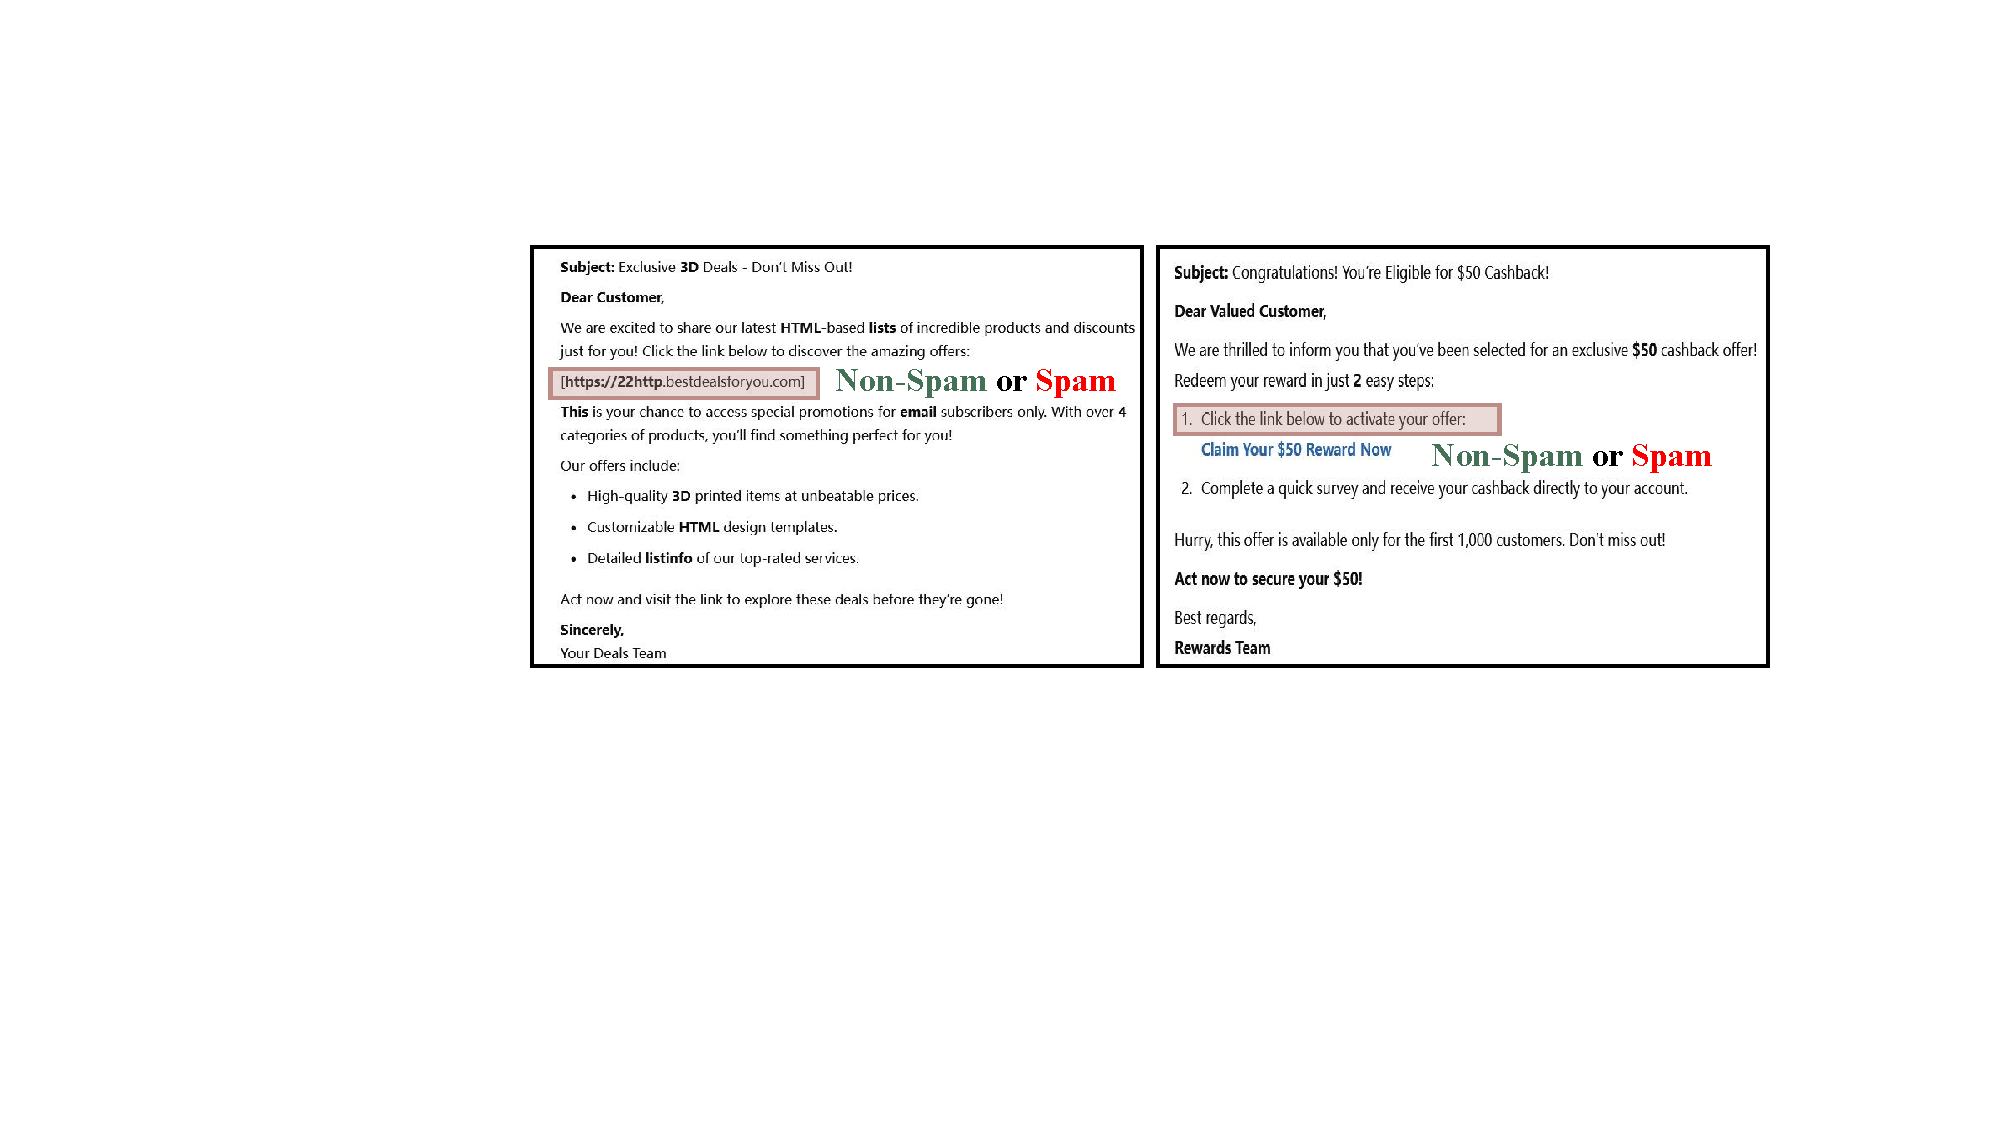
\includegraphics[keepaspectratio,height=3cm]{Graph/Evaluation/SPAM-Dynamics.pdf}
%	\caption{Uncertainty Dynamics in SPAM Email}
%	\label{fig:Uncertainty Dynamics for SPAM}
%\end{figure}
%We selected two feature vectors from spam emails in the SPAM dataset and used AIGC to generate corresponding email content.
%Whether identical feature vectors are classified as spam is not determined by the textual characteristics alone but rather by whether the embedded links are malicious.
%Attackers can exploit this by generating high-uncertainty samples with identical features but opposite labels. Such samples can significantly degrade the concept drift adaptation performance of the target model.
%For example, in spam detection, sample features are word vectors. 
%Using large language models (LLMs), attackers can generate poisoned samples with consistent features but flipped labels, adhering to the clean-label assumption through manual validation, as shown in Equation~\ref{EQ-Guided Untargeted Poisoning Attack}.
%\begin{equation}
%	\begin{aligned}
%		x_{seed}^{t+1} & = \max_{x_{p} \in D_{te}^{t}} uncer\left( x_{p+\alpha}, \theta_{t}^{*} \right)  \\
%		\text{s.t. } &
%		\begin{cases} 
%			uncer\left( x_{p+\alpha}, \theta_{t}^{*} \right)>\beta \\
%			y_{p+\alpha} \neq y_{p}
%		\end{cases}  \\
%	\end{aligned}
%	\label{EQ-Guided Untargeted Poisoning Attack}
%\end{equation}
%
%\subsection{Uncertainty Dynamics based on AIGC}
%\label{Sec: Uncertainty Dynamics based on LLM}
%With the help of generative models, attackers can perturb the uncertainty of existing samples at minimal cost.
%This is particularly significant in domains such as text, images, and videos, where the semantic meaning of labels evolves over time.
%\begin{figure}[htbp]
%	\centering
%	
\includegraphics[width=8cm,height=3cm]{Graph/Evaluation/Figure17-Bird.pdf}
%	\caption{Uncertainty Dynamics based on AIGC (Bird)}
%	\label{fig:Uncertainty Dynamics based on LLM}
%\end{figure}
%Attackers have substantial flexibility in these areas, as the real-world meanings of text and visual entities are constantly evolving.
%As shown in Figure~\ref{fig:Uncertainty Dynamics based on LLM} and Figure~\ref{fig:Uncertainty Dynamics based on LLM-Deer}, we leverage AIGC to quickly generate a series of images with gradually shifting concepts.
%As shown in Figure~\ref{fig:Uncertainty Dynamics based on LLM} and Figure~\ref{fig:Uncertainty Dynamics based on LLM-Deer}, we leverage AIGC to generate images with gradually shifting concepts quickly. 
%\begin{figure}[htbp]
%	\centering
%	
\includegraphics[width=8cm,height=3cm]{Graph/Evaluation/Figure17-deer.pdf}
%	\caption{Uncertainty Dynamics based on AIGC (Deer)}
%	\label{fig:Uncertainty Dynamics based on LLM-Deer}
%\end{figure}
%Attackers do not need to worry about label flipping, as high uncertainty is the core requirement for poisoned samples in PACDA attacks (UPA).
%Furthermore, our experiments on concept drift direction-guided untargeted attacks using the SPAM dataset (Figure~\ref{fig:Untargeted-Attack-Guided}) reveal that label flipping can even enhance the effectiveness of UPA attacks.

%\section{Attacker Cost Analysis}
%\label{Sec: Attacker Cost Analysis}
%
%\noindent The attacker  cost structure is complicated, including manual labeling, poisoned seed sample search, and sample generation costs.
%Since the attacker  surrogate model training phase uses pseudo labels, the active learning process has no manual labeling cost.
%The main labeling cost is used for the search of poisoned samples, which is much smaller than the annotation cost in the active learning process of the victim model, as the attacker only needs to focus on a small number of highly uncertain samples within each test cycle.
%Attackers need to pay a specific cost for the construction of poisoned samples.
%This part involves the construction of the corresponding problem space after the feature space is determined.  
%Large language models can assist attackers in constructing poisoned samples, such as poisoned images and text.
%The problem-space construction of malware samples is inherently more complex.
%However, there are also mature tools available to use~\cite{virboxprotector}.
%We tested mainstream tools and found that the average processing time was 75 seconds per sample.
%The average size of the samples is 199.72MB, and the sample list is shown in Table \ref{tab: APK obfuscation time}. 
%In addition to the fact that automated tools in the industry have significantly reduced the cost of constructing poisoned samples for attackers, existing academic research has shown that related construction is feasible, with the construction time for a single sample being 10 minutes~\cite{2023-CCS-Query-Based-Evasion-Attack}.
%
%\begin{table}[htbp]
%	\centering
%	\small
%	\renewcommand{\arraystretch}{0.8}
%	\caption{APK obfuscation Time}
%	%\renewcommand{\arraystretch}{0.8}  % 璋冩暣璇ヨ〃鏍肩殑琛岃窛
%	\label{tab: APK obfuscation time}
%	\begin{tabular}{c|c|c}
%		\toprule
%		\textbf{APK} & \textbf{Size (MB)} & \textbf{Obfuscation time} \\
%		\midrule
%		JD & 97.59 & 54.95s \\
%		Taobao & 57.03 & 78.98s \\
%		Little Red Book & 162.99 & 178.68s \\
%		Google & 315.67 & 93.32s \\
%		Wang VPN & 45.51 & 14.91s \\
%		WeChat & 264.04 & 136.76s \\
%		\midrule
%		\textbf{Average} & 199.72 & 90.72s \\
%		\bottomrule
%	\end{tabular}
%\end{table} 

%\textcolor{blue}{The time overhead for the attacker is significantly less than the time required for model updating, therefore the attack can be successfully executed.}

%To fully demonstrate the rationality of attack in the problem space, we test the time cost of obfuscation operations.
%We aim to demonstrate that attackers can quickly map poisoned samples from the feature space to the problem space. We select APKs of different types and sizes. 
%Then, we test their repackaging and obfuscation time, as shown in Table \ref{tab: APK obfuscation time}. 
%Based on the time-based test result, we can observe that the average attack time overhead for a single sample in the problem space is less than 5 minutes. 
%Since the concept drift adaptation model is typically updated monthly, attackers have sufficient time to execute PACDA attacks.
% 浠庢鏂囦腑鎽樺嚭鏉ョ殑閮ㄥ垎锛屼篃鏄椂闂村紑閿€鐩稿叧鐨勶紝鏁村悎鍒伴檮褰曞惂
%After fully confirming the effectiveness of the attack method, we conduct tests on the attack time cost, as shown in Table \ref{tab: Attack time cost}.
%We evaluat data from 2013 to 2018 and found that the current optimal concept drift adaptation method has an average feature space attack time cost of 5 minutes and 49 seconds. 
%Because of the different sizes of malware packages, the time cost for problem space attacks varies significantly.
%Therefore, we select various types of software, including e-commerce, gaming, and social media, to test the time cost of problem space attack operations. 
%The experimental results show that the average time cost for a single sample problem space attack operation is 6 minutes and 8 seconds. 
%In summary, the total time cost of the entire attack process is significantly lower than the model update frequency of mainstream concept drift adaptation methods.

%\begin{comment}
%	\begin{table*}[ht]
%		\centering
%		\small
%		\renewcommand{\arraystretch}{0.8}
%		\caption{PACDA Attack time cost}
%		\label{tab: Attack time cost}
%		\begin{tabular}{|c|*{12}{c|}}
%			\toprule
%			\multirow{3}{*}{Stage} & \multicolumn{12}{c|}{Concept Drift Strategy and Active Learning Label Budget} \\
%			\cmidrule{2-13}
%			& \multicolumn{6}{c|}{\textbf{CADE}} & \multicolumn{6}{c|}{\textbf{HCL}} \\
%			\cmidrule{2-13}
%			& 50 & 100 & 150 & 200 & 250 & 300 & 50 & 100 & 150 & 200 & 250 & 300 \\
%			\midrule
%			% 鍦ㄦ澶勬彃鍏ヨ〃鏍兼暟鎹?
%			Seed Selection (Min) & 7.55 & 15.42 & 17.78 & 10.15 & 3.98 & 10.77 & 5.63 & 9.45 & 8.13 & 6.03 & 3.03 & 11.07 \\
%			Sample Generation (Min) & 1.7 & 3.58 & 4.37 & 2.08 & 1.47 & 5.52 & 1.23 & 2.52 & 2.27 & 1.85 & 1.07 & 4.35 \\
%			Model Update (Min) & 4.65 & 4.62 & 5.17 & 5.3 & 1.65 & 3.27 & 1.48 & 1.97 & 1.9 & 1.72 & 0.55 & 2.27\\
%			\midrule
%			\multirow{2}{*}{Stage} & \multicolumn{6}{c|}{\textbf{TRANS}} & \multicolumn{6}{c|}{\textbf{UNC}} \\
%			\cmidrule{2-13}
%			& 50 & 100 & 150 & 200 & 250 & 300 & 50 & 100 & 150 & 200 & 250 & 300 \\
%			\midrule
%			Seed Selection (Min) & 8.63 & 13.2 & 14.93 & 16.29 & 18.15 & 17.77 & 0.08 & 0.1 & 0.06 & 0.08 & 0.08 & 0.12 \\
%			Sample Generation (Min) & 2.52 & 2.63 & 2.82 & 3.05 & 3.17 & 2.57 & 0.1 & 0.03 & 0.03 & 0.03 & 0.1 & 0.2 \\
%			Model Update (Min) & 1.78 & 1.7 & 1.77 & 1.84 & 1.9 & 1.7 & 3.7 & 2.88 & 1.15 & 5.68 & 2.32 & 3.78 \\
%			\bottomrule
%		\end{tabular}
%	\end{table*}
%\end{comment}

%\subsection{Defence Parameter Analysis}
%\label{Sec: Defence Parameter Analysis}
%\noindent \textbf{Activation Clustering (AC)} is a data inspection method. 
%AC assumes the poisoned data in the target class forms a separate cluster that is either small or far from the class center.
%As shown in the Figure~\ref{fig:feature space entanglement}, we utilized the t-SNE tool to visualize the poisoned and non-poisoned samples.
%It can be observed that due to the PACDA attack's use of attack seeds for generating poisoned samples, there is a highly intricate entanglement between poisoned and non-poisoned samples in the feature space.
%As a result, poisoning defense methods based on the AC perform poorly.
%Not only do they fail to eliminate poisoned samples, but they also remove clean samples, thereby undermining the model's ability to generalize effectively.
%\noindent \textbf{(1) Feature Space Entanglement:} As shown in Figure~\ref{fig:feature space entanglement}, t-SNE visualization reveals that PACDA's use of attack seeds creates intricate entanglement between poisoned and clean samples in the feature space (the APIGraph dataset's test data from June 2013).
%Consequently, AC-based defences perform poorly, failing to remove poisoned samples while mistakenly eliminating clean ones, which weakens the model's generalization ability.
%\begin{figure}[htbp]
%	\centering
%	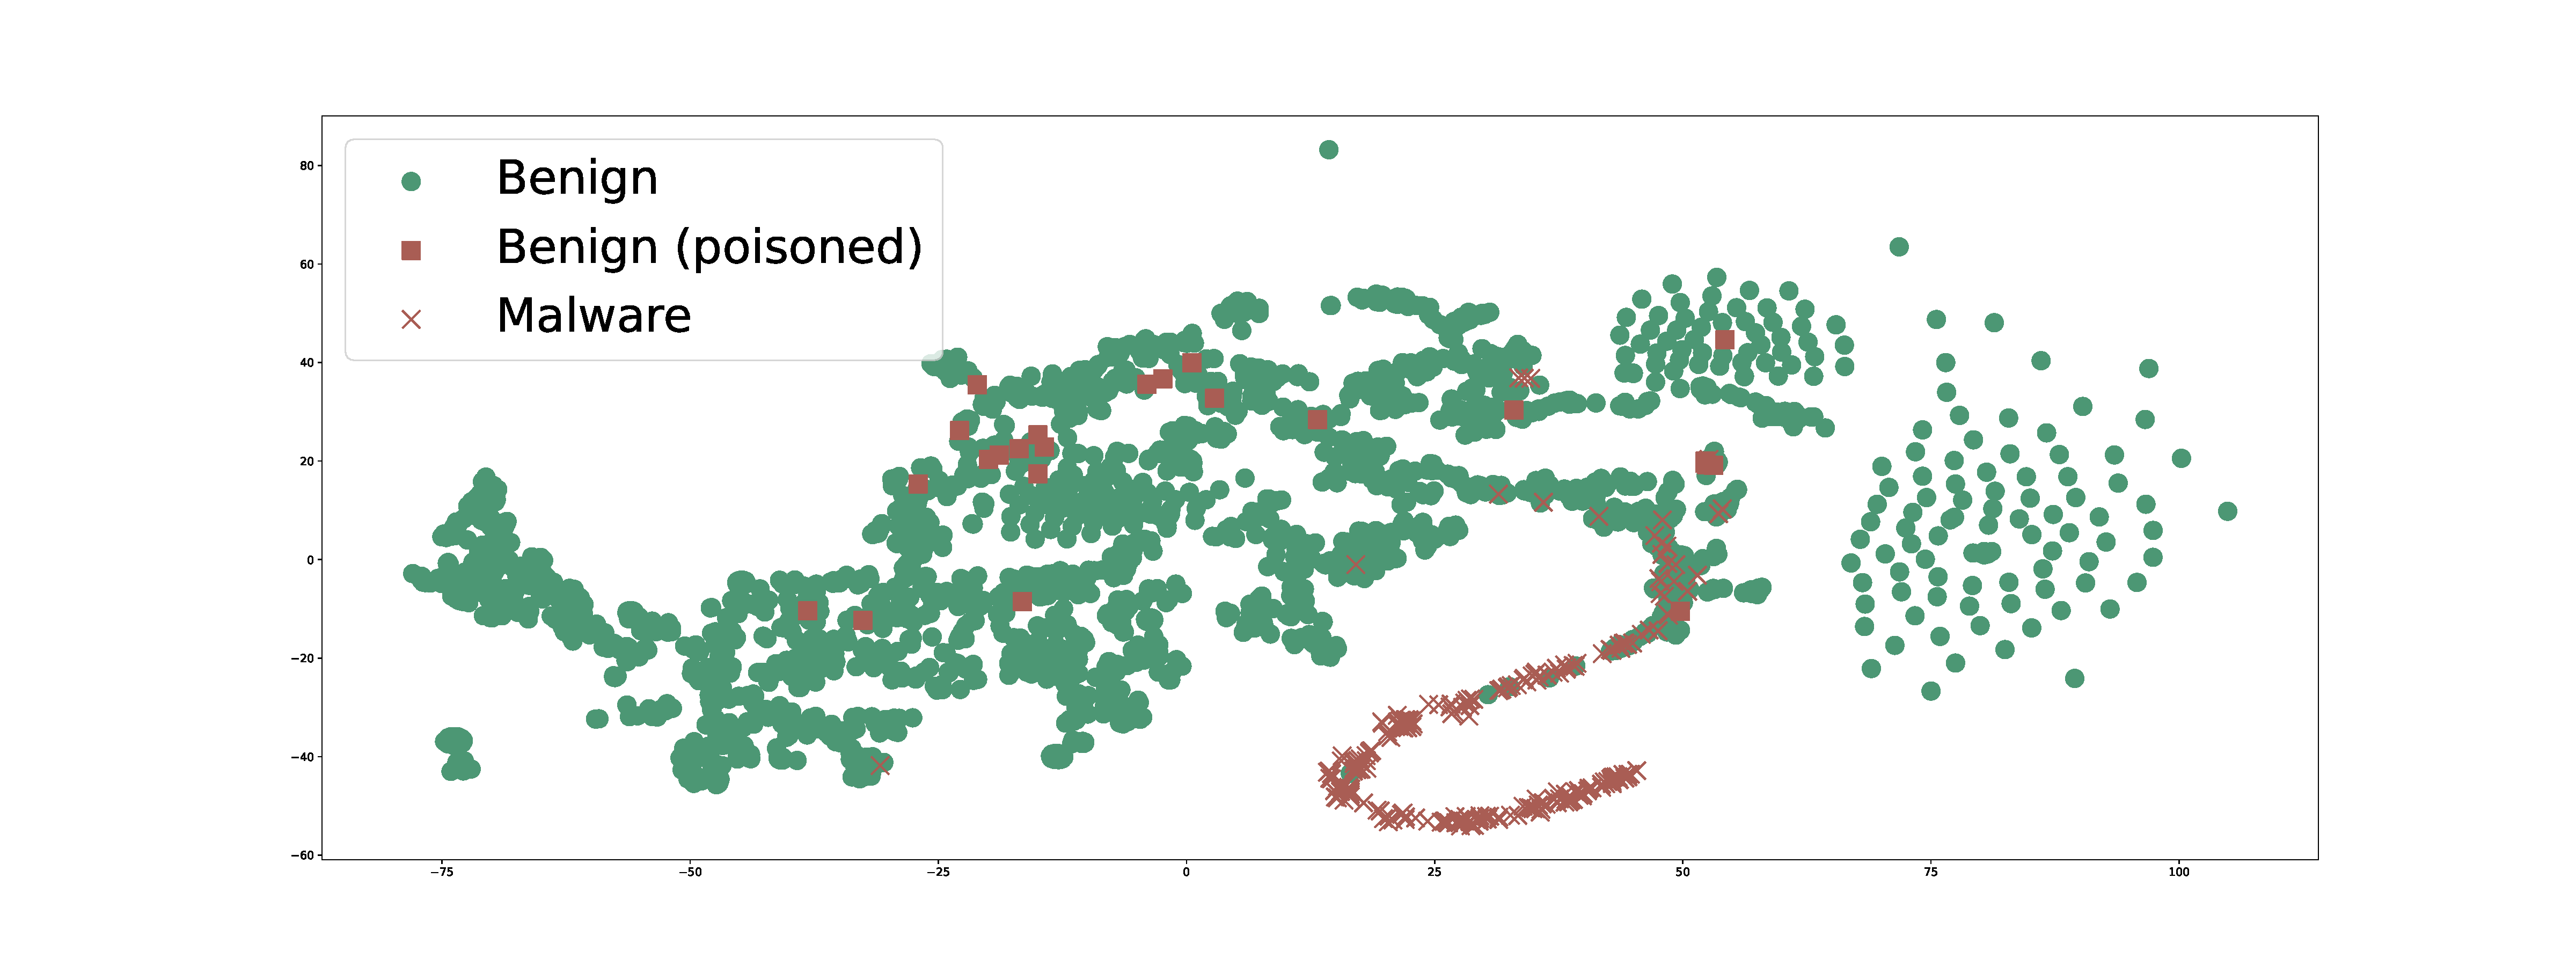
\includegraphics[width=\linewidth,keepaspectratio]{Graph/Evaluation/Figure24-v1}
%	\caption{Feature space entanglement}
%	\label{fig:feature space entanglement}
%\end{figure}
%Due to the longer time span of multi-target attack testing, we selected the APIGraph dataset for defense parameter analysis. 
%The number of clusters was the only parameter requiring manual configuration during the defense.
%We evaluated four cluster settings (6, 10, 20, and 40) under the multi-target attack. 
%The mean F1 score across these four settings was 0.91, with a variance of 0.0025.
%In the single-target attack, we selected the family 'clicks' (with the best ICDF defense performance) and the family 'mogap' (with the worst ICDF defense performance) from the Top 10 attack targets.
%For each family, we conducted four experiments with clustering parameter settings of 6, 10, 20, and 40 and observed that the defense performance remained consistent across all settings.
%This indicates that the defense parameter settings have minimal impact on defense effectiveness, which can effectively reduce the deployment costs of the defense method.

%\section{Practical Significance of PACDA}
%\label{Sec: Practical Significance of PACDA Attacks}
%Attackers can degrade the performance of target models, posing significant threats to the safety of real-world users.
%These risks are particularly severe in sensitive domains such as malware detection and industrial risk analysis, where attacks can lead to financial and physical harm to users.
%In the malware detection scenario studied in this paper, PACDA (under TPA) extends the misclassification duration of specific targets (malware), resulting in longer survival times in real-world scenarios.
%This prolonged survival exacerbates security threats.
%For example, the GriftHorse malware~\cite{GriftHorseMalware}, discovered in November 2020, leveraged subscription-based SMS services to generate 1.5 million USD to 4 million USD in monthly revenue, infecting over 10 million Android devices across 70+ countries.
%If the attacker combines the PACDA attack simultaneously, the harm of the above-mentioned security incident may be further expanded.
%Furthermore, the successful attack targets of PACDA serve as valuable references for attackers in designing future malware, significantly enhancing the efficiency of malware development and amplifying its potential harm.

%\section{Case Study}
%To verify the practicality of leveraging inference uncertainty in real-world machine learning models, we also tested publicly available machine learning services, specifically Baidu's object recognition system~\cite{Baidu-ImageRecognition}. 
%Ten categories from the CIFAR-10 dataset were selected for evaluation.
%Image recognition models show lower uncertainty with single-concept images but higher uncertainty with multi-concept images.
%To explore this, we created conceptual combinations using GAI technologies, enabling attackers to manipulate sample uncertainty in mature machine-learning products.
%The images were generated by progressively increasing the number of conceptual elements, ranging from 1 to 10, with subsequent images incorporating more concepts.
%For detailed information about the images, please refer to Appendix~\ref{Sec: Uncertainty Dynamics based on LLM}.
%\begin{figure}[htbp]
%	\centering
%	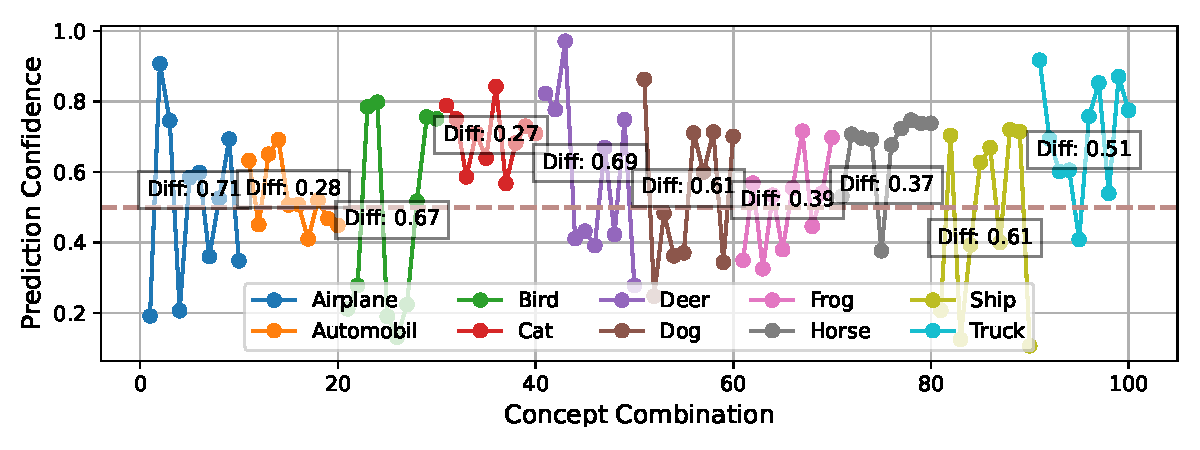
\includegraphics[width=\linewidth,keepaspectratio]{Graph/Evaluation/Figure18.pdf}
%	\caption{Case Study of Uncertainty Dynamics}
%	\label{fig:Case Study of Uncertainty Dynamics}
%\end{figure}
%Figure~\ref{fig:Case Study of Uncertainty Dynamics} illustrates notable fluctuations in sample uncertainty as additional concepts are introduced, with an average range of 0.511 between the highest and lowest uncertainty scores.
%Specifically, 90\% of test categories display uncertainty scores above 0.5 during conceptual combination tests, underscoring the vulnerability of mature machine learning models to manipulations in uncertainty.

%\subsection{Open Science}
%\label{Sec: Open Science}
%\noindent In order to enhance the reproducibility and replicability of scientific findings, we will share our research artifacts. 
%Our code (\url{}) and CDAMAL dataset (\url{https://anonymous.4open.science/r/CDAMAL-Concept-Drift-Dataset-3E08}) are all available. 
%In addition, considering research ethics, our dataset and the source code of the PACDA attack will only share minimized demonstration examples by default to illustrate the attack's effectiveness.

		
		% that's all folks
	\end{document}
	
	
